\documentclass[11pt,a4paper,danish,twoside]{memoir} 
% Skabelon af DTU's LaTeX support gruppe, v20090423
% --------------------------------
\title{Specialkursus}
% --------------------------------
\usepackage[utf8]{inputenc} % Skal passe til editorens indstillinger
\usepackage[danish]{babel} % danske overskrifter
\usepackage{tocvsec2}	
\usepackage[T1]{fontenc} % fonte (output)
\usepackage[table]{xcolor} % farver i tabeller
\usepackage[bottom=4cm]{geometry}
\usepackage{lmodern} % vektor fonte
\usepackage{lipsum} % fyld-tekst
\usepackage{varioref} % referencer
\usepackage{url}	% håndtering af web-adresser
\usepackage{booktabs} % pæne tabeller
\usepackage{topcapt} % captions til tabeller
\usepackage{threeparttable}	% tabel-noter
\usepackage[referable]{threeparttablex} % tabel-noter i longtables
\usepackage{longtable}	% tabeller over flere sider
\usepackage{rotating}
\usepackage{lscape}
\usepackage{multirow} % fletning af rækker i tabeller
\usepackage{dcolumn} % justering af kolonner
\usepackage{graphicx} % indsættelse af billeder
\usepackage[export]{adjustbox} % rammer om billeder
\usepackage{tikz} % tegn på billeder
\usepackage{pgfplots}
\usepackage[round]{natbib}
\usepackage{gensymb} % celcius og grader
\usepackage{amsmath} % celcius
\usepackage{siunitx} % vinkler
\usepackage[url]{dk-bib}
\usepackage{titlesec}
\usepackage{wallpaper}
\usepackage{caption}	%	Justering af figur-tekster
% \usepackage[3D]{movie15} % 3D illustration i pdf-format
\usepackage{subcaption} 
\usepackage[final]{pdfpages} % inkludere pdf filer
%\usepackage{hyperref}
\usepackage{textcomp} % bla. celcius
\usetikzlibrary{patterns} % muligheder for mønstre i tikz
\titlespacing{\paragraph}{0pt}{15pt}{.4em}[]
%% Make \cite default to \citep instead
\let\cite\citep
\pgfplotsset{compat=newest}
\let\vref\ref

\hyphenation{Si-mon-sen}

% -------------------------	
\settocdepth{section} % justering af indholdsfortegnelse
\setsecnumdepth{subsection}
\maxsecnumdepth{subsection}
% -------------------------
\usepackage{chngcntr}	% skift nummerering af tabeller og figurer i appendix
\graphicspath{{./billeder/}} % stivej til bibliotek med figurer

\usepackage[colorinlistoftodos]{todonotes}	% pakke til noter
%\usepackage[disable]{todonotes}	% fjern todos fra PDF
% todo-farver
\definecolor{anders}{RGB}{255,255,0}
\definecolor{darkgreen}{RGB}{0,153,0}
\definecolor{forslag}{RGB}{100,150,250}

%	VREF
\vrefwarning

\usepackage{mathtools} % matematik - understøtter muligheden for at bruge \eqref{}https://preview.overleaf.com/public/ndkwnwsgspxv/images/8801bcf52a084e52bb85dcbdcf72354cc80de42c.jpeg
\usepackage{siunitx}
\sisetup{per-mode=symbol-or-fraction}
\usepackage{icomma}
\usepackage[plainpages=false,pdfpagelabels,pageanchor=false]{hyperref} % aktive links
\usepackage{memhfixc}% rettelser til hyperref

\usepackage{enumitem}
\setlist[enumerate]{label*=\arabic*.}	% 

\usepackage[framemethod=tikz]{mdframed}
\newmdenv[tikzsetting={draw=black,fill=white,fill opacity=0.7},backgroundcolor=none]{myenvironment}

% ------------------------------------------
%	Lay-out
% --------------------------------------
%%	Pagestyle
%\usepackage{fancyhdr}
\pagestyle{companion}

%	Chapterstyle
\chapterstyle{section}

%	Figurtekst
\captionsetup{font=small,labelfont=bf}
%format = hang
%textfont=sf
% ------------------------------------------


% ------------------------------------------
% Kompiler kun de kapitler du arbejder med.
% --------------------------------------
% \includeonly{	
%}
% ------------------------------------------

\begin{document}
\frontmatter % sidenumre som romertal
\pagenumbering{Roman}
% \maketitle  % bruges hvis man ikke har sin egen forside
 

% \include{resume}

%\listoftodos[To do Notes]
\newgeometry{top=3cm,bottom=2.5cm,left=2.5cm,right=2.5cm}
\begin{titlingpage}

\begin{myenvironment}
\centering \parindent=0pt
\newcommand{\HRule}{\rule{\textwidth}{1mm}}
\vspace*{\stretch{1}} \HRule\\[1cm]\Huge\bfseries
Klassifikation af isindhold i permafrostkerner \\[0.7cm]
\large - et metodestudie\\[1cm]
\HRule\\[1cm]  \large af Anders Halsne Sand, s122970\\
\vspace*{\stretch{2}} \normalsize %
\end{myenvironment}
\vfill
\begin{myenvironment}
\begin{flushleft}
Danmarks Tekniske Universitet\\
Institut for Byggeri og Anlæg\\
Diplom Afgangsprojekt\\
Vejleder: Thomas Ingeman-Nielsen\\
\today \end{flushleft}
\end{myenvironment}

% \ThisTileWallPaper{\paperwidth}{\paperheight}{frontpage}
\end{titlingpage}
\restoregeometry
\chapter{Forord}
Denne rapport er udarbejdet som et speciale kursus, der indgår som sidste del af min diplomingeniør uddannelsen Arktisk Teknologi ved Center for Arktisk Teknologi (Artek), DTU Lyngby, med Thomas Ingeman-Nielsen som vejleder. Specialekursuset har en belastning på 15 ECTS point, fordelt på forsøgvejledning for bestemmelse af bulkdensitet ved arkimedes princip og 3D scanner, laboratorieforsøg, resultatbehandling samt en vurdering af laboratorieforsøg.

\noindent Rapporten tager udgangspunkt i et ønske om at finde en ny og ikke-destruktiv metode til at bestemme bulkdensitet af permafrostkerner. 

\noindent Alle prøver anvendt i denne rapport tilhører Geo og indholdet skal håndteres fortroligt. 


\chapterstyle{reparticle}
\tableofcontents*
\newpage
\listoffigures*
\newpage
\listoftables*
\chapterstyle{section}

\mainmatter % arabiske sidenumre

% \newgeometry{top=3cm,bottom=2.5cm,left=2.5cm,right=2.5cm}
\begin{titlingpage}

\begin{myenvironment}
\centering \parindent=0pt
\newcommand{\HRule}{\rule{\textwidth}{1mm}}
\vspace*{\stretch{1}} \HRule\\[1cm]\Huge\bfseries
Klassifikation af isindhold i permafrostkerner \\[0.7cm]
\large - et metodestudie\\[1cm]
\HRule\\[1cm]  \large af Anders Halsne Sand, s122970\\
\vspace*{\stretch{2}} \normalsize %
\end{myenvironment}
\vfill
\begin{myenvironment}
\begin{flushleft}
Danmarks Tekniske Universitet\\
Institut for Byggeri og Anlæg\\
Diplom Afgangsprojekt\\
Vejleder: Thomas Ingeman-Nielsen\\
\today \end{flushleft}
\end{myenvironment}

% \ThisTileWallPaper{\paperwidth}{\paperheight}{frontpage}
\end{titlingpage}
\restoregeometry
\chapter{Indledning}
Den metode der indtil nu har været andvendt til at bestemme densitet af permafrostkerner er Archimedes princip, hvor kernen nedsænkes i Isopar. Metoden bestemmer densiteten præcist, men deler af prøven bliver påvirket, da Isoparen trænger ind i kernen, og kernen kan derfor ikke anvendes til andre forsøg bagefter. Af denne grund er det interessant at se på andre alternativer som ikke er destruktive, til bulkdensitets bestemmelse af permafrostkerner. I denne rapport bliver bulkdensiteten bestemt ud fra Archimedes princip, samt ved fotogrammetri-struktureret lys metoden, de samme kerner, anvendes til begge formål, og resultaterne sammenlignes.    
\chapter{Teori}
I det følgende kapitel er en kort beskrivelse af 3D scanning - Struktureret Lys, og de principper metoden anvender. Sidst i kapitlet er der en kort introduktion til  Archimedes princip. 

\section{Fotogrammetri - struktureret lys}
3D-billedbehandling referer til teknikker som giver reel 3D data af et objekt. Der findes flere metoder som kan dette, valget af metode er afhængig af hvilken data der ønskes. Struktureret lys metoden er en metode der anvender en projektor samt et eller flere kameraer, hvor projektøren sender et struktureret lys på det emnet der ønskes information om. Metoden samler data om emnets overflade, hvilket kan andvendes til flere formål, som f.eks. volumenberegning og 3D printing. I denne rapport bliver struktureret lys andvendt til at lave volumenberegninger på permafrostkerner.
% Struktureret lys er en form for overfladeafbildning af et objekt, hvor punkter på objektets overflade bliver illustreret i et koordinatsystem (x,y,z).
% Hvor z-koordinaterne er en fuktion af (x,y) koordinaterne i et kartesiske koordinatsystem, og kan udtrykkes i matrice form som:
% ${z_{ij}=(x_i,y_j,)i=1,2...,L,j=1,2...,M}$.
Ved 3D-billedbehandlings system er det muligt at erhverve en skalar-værdi som en reflekterende overflade, associeret med et punkt på den ikke-plane overflade, hvilket resulterer i en punkt-sky der beskrives ved: $P_i=(x_i,y_i,z_i,f_i),i=1,2...,N$, hvor $f_i$ repræsenterer værdien af overfladepunktet i, i data sættet. Ligeledes repræsenteres farver ved: $P_i=(x_i,y_i,z_i,r_i,g_i,b_i),i=1,2...,N$, hvor vektorene $r_i$,$g_i$ og $b_i$ repræsenterer farvene illustreret på figur \vref{fig:opst_strukt_lys} (rød, grøn og blå), i det givne overfladepunkt (i). 
Ved struktureret lys metoden belyses et objektet med et specielt designet 2D rumligt varierende mønster, som vist på figur \vref{fig:opst_strukt_lys}, hvor den rumligt varierende 2D struktureret belysning genereret af en projektor designet til det formål, eller en anden lyskilde moduleret af en rumlig lysmodulator (Geng,2011).

Intensiteten af hvert piksel på det strukturerede lys-mønster er repræsenteret av et digitalt signal: $I_{ij}=(i,j),i=1,2,...,I,j=1,2,...,J$, hvor (i,j) repræsenterer (x,y) koordinaterne til det projekterende mønster.
En billede sensor som f.eks. et kamera anvendes til at optage 2D bilede af det strukturerede lys. Hvis det er tale om en plan overflade uden 3D variation, er det strukturede mønster fanget af kamera ens med det projekterende lys. Hvis der er tale om et rumlig objekt, vil overfladen af objektet forvrænge det projekterende lys, der fanges af kameraet. Princippet ved strukturered lys 3D billedbehandlingssytem er at indsamle 3D information fra det forvrængede lys.Geometrienaf objektet kalkuleres ved brug af struktureret lys principper og algoritmer. Ved brug af triangulering kan det geometriske forhold mellem bildesensoren (kamera), projektor og hvert enkelt punktet på objektets overflade, se figur \vref{fig:opst_strukt_lys}, kan udtrykkes ved formel: \vref{eq:triangulering_kam} (Geng,2011). 

%
\begin{equation}
R=B*\frac{sin(\theta)}{sin(\alpha+\theta)}
\label{eq:triangulering_kam}
\end{equation}
%


%Struktureret lys skanning, er en form for fotogrammetri som er en alsidig metode til at opnåelse af 3D form. Almindelige kameraer kan kun optage 2D, da de mangler dybde information. Ved struktureret lys metoden, anvendes der samtidig en projektor der lægger et mønster over det objekt der ønsker information om.  

\begin{figure}
\centering
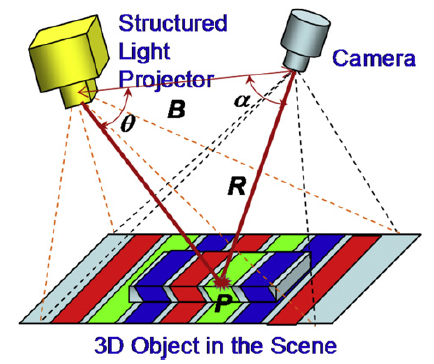
\includegraphics[width=0.6\textwidth]{Unavngivet}
\caption{Opstilling-struktureret lys (Geng,2011).}
\label{fig:opst_strukt_lys}
\end{figure}
  

% %
% \begin{figure}
% \centering
% %%%% BEGIN DOCUMENT
%\begin{document}
%
%
%
%

\begin{tikzpicture}
%%%% -----------Stativ + holder-------------%%%%
% \draw [gray, ultra thick]	(-4,-4) -- (-2,-4)	 			;		
% \draw [gray, ultra thick]	(-3,-4) -- (-3,4)	 			;		
% \draw [gray, ultra thick]	(-3,4) -- (1,4)					;
% \draw [gray, ultra thick]	(1,4) -- (1,0)					;
% \draw [black, ultra thick]	(1,0) -- (0,-2)					;
% \draw [black, ultra thick]	(1,0) -- (2,-2)					;
% \draw [black, ultra thick]	(0,-2) -- (2,-2)					;

%%%----------Vægt---------%%%
% \draw [gray, ultra thick]	(0,-2.7) -- (2,-2.7)			;
% \draw [gray, ultra thick]	(0,-2.7) -- (0,-2.9)			;

% \draw [gray, ultra thick]	(-0.5,-2.9) -- (2.5,-2.9)		;
% \draw [gray, ultra thick]	(2.0,-2.7) -- (2.0,-2.9)		;
% \draw [gray, ultra thick]	(-0.5,-2.9) -- (2.5,-2.9)		;

% \draw [gray, ultra thick]	(-0.5,-4) -- (3.5,-4)			;
% \draw [gray, ultra thick]	(-0.5,-2.9) -- (-0.5,-4.0)		;
% \draw [gray, ultra thick]	(2.5,-2.9) -- (3.5,-4)			;
% \node at (1.0,-3.5) {Vægt} 									;


%%%%------------Prøve----------------%%	
\draw[red, ultra thick, pattern=north east lines, pattern color=gray] (1.0,-2) circle [radius=0.5] ;
% \draw [red, ultra thick] (1.0,1.5) circle [radius=0.5]		;
\node [right] at (4.0,-2) {Prøveemne}						;
\draw [->] (3.9,-2) -- (2.0,-2);
%%%%------------Beholder Isobar----------------%%	
\draw [black, ultra thick]	(-0.5,0.5) -- (-0.5,-2.5)	 		;	
\draw [black, ultra thick]	(2.5,0.5) -- (2.5,-2.5)	 			;
\draw [black, ultra thick]	(-0.5,-2.5) -- (2.5,-2.5)	 		;
% \node at (1.0,-1.0) {Isopar} ;
\node [right] at (4.0,-1){Beholder}			 ;
\draw [->] (3.9, -1) -- (2.7,-1)							 ;



%%%-------------Kurve-------------%%%
% \draw[ultra thick, blue]
%     (-0.5,0.0) sin (-0.25,0.25) cos(0.0,0) sin (0.25,-0.25) cos(0.5,0.0) sin(0.75,0.25) cos(1,0.0) sin(1.25,-0.25) cos(1.5,0.0) sin(1.75,0.25) cos(2.0,0.0) sin(2.25,-0.25) cos(2.5,0.0);

 \draw[dashed, thick, blue] 
	(-0.5,0) -- (2.5,0)	;
 \draw[ultra thick,blue] 
 (-0.5,0.25) -- (2.5,0.25)	;
% \node [above] at (-1.5,2) {Temperaturføler}		;

% %%%-----------Føler-----------%%%
% %\draw [green, thick] (-0.0,-1) -- (-0.0,-2.5);
% \draw[gray, dashed] (-0.25,-0.5) -- (-0.25,0.5);
% \draw[gray, dashed] (-0.25,0.5) to [out=90, in = 0] (-2,2)		;

% \draw [ultra thick, green] (-0.25,-0.5) -- (-0.25,-1.5) 		;
   

% \node [left,black] at (-4,-4) {$L_1$}							;
% \node [right,black] at (1.5,1.5) {$L_2$}						;
% \node [below left,black] at (-2,1) {$d_{1,1}$}				;
% \node [above right,black] at (2,-1) {$d_{1,2}$}				;
% \node [below right,black] at (1.25,1.25) {$d_{2,1}$}						;
% \node [above left,black] at (-0.25,-0.25) {$d_{2,2}$}			;

%%%---------- Hjelpe linjer ------------%%%

%   \draw [help lines] (-5,-5) grid (5,5);
%   \draw [help lines, step = 2,ultra thick] (-5,-0) grid (5,0);
%   \draw [help lines, step = 2,ultra thick] (-0,-5) grid (0,5);
%%%%%
\end{tikzpicture}



%\end{document}
% \caption{Nedsænkning af et legeme i en væske}
% \label{fig:arki_ops_veske_teori}
% \end{figure}
% %

\section{Opdrift og Archimedes princip}
Archimedes princip omhandler kræfters påvirkning af et legeme ned-sænket i en væske. Et legeme nedsænket i væske påvirkes af tyngdekraften $F_g$ samt en opadrettet kraft (opdrift) $F_o$, hvor opdriften, svarer til vægten af den fortrængte væske, $m_for$, dette under forudsætning at væsken ikke er i bevægelse. 
Ved at nedsænke et legeme med en kendt masse og volumen, kan en væskes densitet bestemmes. Når væskens densitet kendes, kan volumen bestemmes af et hvilket som helst legeme såfremt det nedsænkes i den samme væske, under samme forhold.(Fishbane et al. 1996) 

Når et legeme flyder højt, som i figur \vref{fig:arki_fop} gælder fælgende forudsætniger: 
%
\begin{equation} 
 V^\prime< V
\end{equation}
% 
% 
\begin{equation} 
 F_o=\rho_v*V^\prime=F_g=\rho*V
\end{equation}
% 
% 
\begin{equation} 
 \frac{V^\prime}{V}=\frac{\rho}{\rho_v}
\end{equation}
% 
Hvor $V^\prime$ er det fortrængte volumen, $F_g$ er gravitation, $F_o$ er opdrift, $V$ er objektets totale volumen, $\rho_v$ er væskens densitet, og den totale kraft der påvirker objektet $F_{tot}=0$. 
%
\begin{figure}
\centering
%%%% BEGIN DOCUMENT
%\begin{document}
%
%
%
%

\begin{tikzpicture}

%%%%------------Prøve----------------%%	
\draw[red, ultra thick, pattern=north east lines, pattern color=gray] (1.0,0) circle [radius=0.5] ;
% \draw [red, ultra thick] (1.0,1.5) circle [radius=0.5]		;
\node [right] at (4.0,0.25) {Prøveemne}						;
\draw [->] (3.9,0.25) -- (1.7,0.25)								;
\node [left] at (0.25,0.8) {$\mathbf{{F}_{o}}$}			;
\draw [ultra thick][->] (0.4,0.1)--(0.4,1)				;
\node [left] at (0.25,-0.8) {$\mathbf{{F}_{g}}$}			;
\draw [ultra thick][->] (0.4,-0.1)--(0.4,-1.0)				;

%%%%------------Beholder Isobar----------------%%	
\draw [black, ultra thick]	(-0.5,0.5) -- (-0.5,-2.5)	 		;	
\draw [black, ultra thick]	(2.5,0.5) -- (2.5,-2.5)	 			;
\draw [black, ultra thick]	(-0.5,-2.5) -- (2.5,-2.5)	 		;
% \node at (1.0,-1.0) {Isopar} ;
\node [right] at (4.0,-1){Beholder}			 ;
\draw [->] (3.9, -1) -- (2.7,-1)							 ;

% {$\mathbf{M}_{ji}$} (j)

%%%-------------Kurve-------------%%%

%  \draw[dashed, thick, blue] 
% 	(-0.5,0) -- (2.5,0)	;
 \draw[ultra thick,blue] 
 	(-0.5,0.0) -- (0.47,0.0)	;
 \draw[dashed, thick, blue] 
 	(0.5,0.0) -- (1.5,0)	;
 \draw[ultra thick,blue] 
 (1.53,0.0) -- (2.5,0.0)	;
\node [right] at (4.0,-2) {Væske}						;
\draw [->] (3.9,-2) -- (2.2,-2)								;


%%%---------- Hjelpe linjer ------------%%%

%    \draw [help lines] (-5,-5) grid (5,5);
%    \draw [help lines, step = 2,ultra thick] (-5,-0) grid (5,0);
%    \draw [help lines, step = 2,ultra thick] (-0,-5) grid (0,5);
%%%%%
\end{tikzpicture}

\caption{Legeme der flyder-$F_{tot}=op$}
\label{fig:arki_fop}
\end{figure}
%
For et legeme der flyder i overfladen som vist på figur \vref{fig:arki_foverflade}, gælder følgende principper:
% 
\begin{equation}
V^\prime=V
\end{equation}
%
% 
\begin{equation}
\rho=\rho_v
\end{equation}
% 
Hvor de to volumener og densitet er ens, og $F_{tot}=0$.
% 
% 
\begin{figure}
\centering
%%%% BEGIN DOCUMENT
%\begin{document}
%
%
%
%

\begin{tikzpicture}

%%%%------------Prøve----------------%%	
\draw[red, ultra thick, pattern=north east lines, pattern color=gray] (1.0,-0.5) circle [radius=0.5] ;
% \draw [red, ultra thick] (1.0,1.5) circle [radius=0.5]		;
\node [right] at (4.0,-0.5) {Prøveemne}						;
\draw [->] (3.9,-0.5) -- (1.7,-0.5)								;
\node [left] at (0.25,0.4) {$\mathbf{{F}_{o}}$}			;
\draw [ultra thick][->] (0.4,-0.4)--(0.4,0.5)				;
\node [left] at (0.25,-1.3) {$\mathbf{{F}_{g}}$}			;
\draw [ultra thick][->] (0.4,-0.6)--(0.4,-1.54)				;

%%%%------------Beholder Isobar----------------%%	
\draw [black, ultra thick]	(-0.5,0.5) -- (-0.5,-2.5)	 		;	
\draw [black, ultra thick]	(2.5,0.5) -- (2.5,-2.5)	 			;
\draw [black, ultra thick]	(-0.5,-2.5) -- (2.5,-2.5)	 		;
% \node at (1.0,-1.0) {Isopar} ;
\node [right] at (4.0,-1){Beholder}			 ;
\draw [->] (3.9, -1) -- (2.7,-1)							 ;

% {$\mathbf{M}_{ji}$} (j)

%%%-------------Kurve-------------%%%

%  \draw[dashed, thick, blue] 
% 	(-0.5,0) -- (2.5,0)	;
 \draw[ultra thick,blue] 
 	(-0.5,0.0) -- (2.5,0.0)	;
%  \draw[dashed, thick, blue] 
%  	(0.5,0.0) -- (1.5,0)	;
%  \draw[ultra thick,blue] 
%  (1.53,0.0) -- (2.5,0.0)	;
 \node [right] at (4.0,-2) {Væske}						;
 \draw [->] (3.9,-2) -- (2.2,-2)								;


%%%---------- Hjelpe linjer ------------%%%

%    \draw [help lines] (-5,-5) grid (5,5);
%    \draw [help lines, step = 2,ultra thick] (-5,-0) grid (5,0);
%    \draw [help lines, step = 2,ultra thick] (-0,-5) grid (0,5);
%%%%%
\end{tikzpicture}

\caption{Legeme nedsunken i væske - $F_{tot}=0$}
\label{fig:arki_foverflade}
\end{figure}
%
% 
Når objektet synker, eller er fuldstendig neddykket som vist på figur \vref{fig:arki_fdown} gælder følgende forudsætninger:

% 
\begin{equation}
V^\prime=V
\end{equation}
% 
% 
\begin{equation}
\rho>\rho_v
\end{equation}
% 
Volumen af den neddykede objekt er det samme som volumen af den fortrængte væske, densiteten af objektet er større en densiteten af væsken, hvilket medfører at objektet synker (Fishbane et al. 1996). 
%
\begin{figure}
\centering
%%%% BEGIN DOCUMENT
%\begin{document}
%
%
%
%

\begin{tikzpicture}

%%%%------------Prøve----------------%%	
\draw[red, ultra thick, pattern=north east lines, pattern color=gray] (1.0,-1) circle [radius=0.5] ;
% \draw [red, ultra thick] (1.0,1.5) circle [radius=0.5]		;
\node [right] at (4.0,-1) {Prøveemne}						;
\draw [->] (3.9,-1) -- (1.7,-1)								;
\node [left] at (0.25,-0.4) {$\mathbf{{F}_{o}}$}			;
\draw [ultra thick][->] (0.4,-0.9)--(0.4,-0.1)				;
\node [left] at (0.25,-1.4) {$\mathbf{{F}_{g}}$}			;
\draw [ultra thick][->] (0.4,-1.1)--(0.4,-1.9)				;

%%%%------------Beholder Isobar----------------%%	
\draw [black, ultra thick]	(-0.5,0.5) -- (-0.5,-2.5)	 		;	
\draw [black, ultra thick]	(2.5,0.5) -- (2.5,-2.5)	 			;
\draw [black, ultra thick]	(-0.5,-2.5) -- (2.5,-2.5)	 		;
% \node at (1.0,-1.0) {Isopar} ;
\node [right] at (4.0,-1.5){Beholder}			 ;
\draw [->] (3.9, -1.5) -- (2.7,-1.5)							 ;

% {$\mathbf{M}_{ji}$} (j)

%%%-------------Kurve-------------%%%

%  \draw[dashed, thick, blue] 
% 	(-0.5,0) -- (2.5,0)	;
 \draw[ultra thick,blue] 
 (-0.5,0.0) -- (2.5,0.0)	;
 \node [right] at (4.0,-2) {Væske}						;
\draw [->] (3.9,-2) -- (2.2,-2)								;



%%%---------- Hjelpe linjer ------------%%%

%    \draw [help lines] (-5,-5) grid (5,5);
%    \draw [help lines, step = 2,ultra thick] (-5,-0) grid (5,0);
%    \draw [help lines, step = 2,ultra thick] (-0,-5) grid (0,5);
%%%%%
\end{tikzpicture}

\caption{Legeme der synker-$F_{tot}=ned$}
\label{fig:arki_fdown}
\end{figure}
%
% %%%% BEGIN DOCUMENT
%\begin{document}
%
%
%
%

\begin{tikzpicture}
%%%% -----------Stativ + holder-------------%%%%
\draw [gray, ultra thick]	(-4,-4) -- (-2,-4)	 			;		
\draw [gray, ultra thick]	(-3,-4) -- (-3,4)	 			;		\draw [gray, ultra thick]	(-3,4) -- (1,4)					;
\draw [gray, ultra thick]	(1,4) -- (1,3)					;
\draw [black, ultra thick]	(1,3) -- (0,1)					;
\draw [black, ultra thick]	(1,3) -- (2,1)					;
\draw [black, ultra thick]	(0,1) -- (2,1)					;

%%%----------Vægt---------%%%
\draw [gray, ultra thick]	(0,-2.7) -- (2,-2.7)			;
\draw [gray, ultra thick]	(0,-2.7) -- (0,-2.9)			;

\draw [gray, ultra thick]	(-0.5,-2.9) -- (2.5,-2.9)		;
\draw [gray, ultra thick]	(2.0,-2.7) -- (2.0,-2.9)		;
\draw [gray, ultra thick]	(-0.5,-2.9) -- (2.5,-2.9)		;

\draw [gray, ultra thick]	(-0.5,-4) -- (3.5,-4)			;
\draw [gray, ultra thick]	(-0.5,-2.9) -- (-0.5,-4.0)		;
\draw [gray, ultra thick]	(2.5,-2.9) -- (3.5,-4)			;
\node at (1.0,-3.5) {Vægt} 									;


%%%%------------Prøve----------------%%	
\draw[red, ultra thick, pattern=north east lines, pattern color=gray] (1.0,1.5) circle [radius=0.5] ;
% \draw [red, ultra thick] (1.0,1.5) circle [radius=0.5]		;
\node [right] at (4.0,1.5) {Prøveemne}						;
\draw [->] (3.9, 1.5) -- (2.0,1.5);
%%%%------------Beholder Isobar----------------%%	
\draw [black, ultra thick]	(-0.5,0.5) -- (-0.5,-2.5)	 		;	
\draw [black, ultra thick]	(2.5,0.5) -- (2.5,-2.5)	 			;
\draw [black, ultra thick]	(-0.5,-2.5) -- (2.5,-2.5)	 		;
\node at (1.0,-1.0) {Isopar} ;
\node [right] at (4.0,0.5){Beholder}			 ;
\draw [->] (3.9, 0.5) -- (2.7,0.5)							 ;



%%%-------------Kurve-------------%%%
% \draw[ultra thick, blue]
%     (-0.5,0.0) sin (-0.25,0.25) cos(0.0,0) sin (0.25,-0.25) cos(0.5,0.0) sin(0.75,0.25) cos(1,0.0) sin(1.25,-0.25) cos(1.5,0.0) sin(1.75,0.25) cos(2.0,0.0) sin(2.25,-0.25) cos(2.5,0.0);

\draw[ultra thick, blue] 
	(-0.5,0) -- (2.5,0)	;
\node [above] at (-1.5,2) {Temperaturføler}		;

%%%-----------Føler-----------%%%
%\draw [green, thick] (-0.0,-1) -- (-0.0,-2.5);
\draw[gray, dashed] (0.00,-0.5) -- (0.00,0.5);
\draw[gray, dashed] (0.00,0.5) to [out=90, in = 0] (-2,2)		;

\draw [ultra thick, green] (0.00,-0.5) -- (0.00,-1.5) 		;
   

% \node [left,black] at (-4,-4) {$L_1$}							;
% \node [right,black] at (1.5,1.5) {$L_2$}						;
% \node [below left,black] at (-2,1) {$d_{1,1}$}				;
% \node [above right,black] at (2,-1) {$d_{1,2}$}				;
% \node [below right,black] at (1.25,1.25) {$d_{2,1}$}						;
% \node [above left,black] at (-0.25,-0.25) {$d_{2,2}$}			;

%%%---------- Hjelpe linjer ------------%%%

% \draw [help lines] (-5,-5) grid (5,5);
% \draw [help lines, step = 2,ultra thick] (-5,-0) grid (5,0);
% \draw [help lines, step = 2,ultra thick] (-0,-5) grid (0,5);
%%%%%
\end{tikzpicture}



%\end{document}
\FloatBlock
\chapter{Metode}
I dette kapitel beskrives metoderne bag indsamling af data, samt processering af data. Først kommer en beskrivelse af udvælgelse af prøveemner, derefter følger en kort beskrivelse af klassifikationsbestemmelse baseret på en visuel inspection. Derefter følger en beskrivelse af den fotogrammetrisk oppstilling samt efterbehandlig af data anvendt til bulkdensitets bestemmelse, til sidst i kapitlet kommer en beskrivelse af metoden for archimedes princip og opstillingen brugt til bulkdensitets bestemmelse. Alle forsøg udføres i klimakammer ved en temperatur på -6 $\celsius$ ved, DTU - Lyngby. 
%%% ---------- UDVÆLGELSE  AF PRØVEEMNER ---------- %%%
\section{Udvælgelse af prøveemner}
Der bestemmes bulk densitet på 15 prøver, hvilke prøver det er og hvilke boringer de tages fra er forudbestemt. Bulk densitet bestemmelserne ligger til grunde for valg af kerner der på et senere bliver udvalgt oedometer og triaksial -forsøg. 

\noindent Bulkdensiteten bestemmes ved to uafhængige forsøg, i det første forsøg anvendes 3D scanning- struktureret lys metoden, og i det andet forsøg anvendes Archimedes princip, de samme prøveemner anvendes til de to forsøg.

Ved 3D scanningen er der valgt at alle 15 prøver scannes ved en rotationsvinkel på 45 grader, derudover er der udvalgt fire prøver som itlleg scannes ved en rotationsvinkel på 60 og 72 -grader. De fire prøver er udvalgt baseret på visuel inspektion samt masse [g]. 

Formålet ved at anvende forskellige rotationsvinker er å se om vinkelen påvirker resultatet af den afledte densitet. 
I forkant har, test-scanning udføret på DTU-Compute, vist at scannings metoden baseret på struktureret lys har svært ved at håndtere is, af dene grund er der valgt prøver to prøver som antages at have det højeste isindhold af de 15 prøveemner. Derudover er der valgt to prøver der antages at have lavt isindhold.

Derudover er der lagt vægt på at prøveemnerne har samme kernediameter. I prøvepopulationen har 12 prøver en kernediameter på $70 mm$ og tre prøver på $50 mm$. Da det ikke vides på forhånd om prøvens strørrelse har betydning for resultatet af scanningen vælges prøver af samme kernediameter. De fire prøver udvalgt til scanning ved alle rotationsvinkler samt begrundelse, henvises der til tabel \vref{tab:valg_prover}.

%
\begin{table}
\centering
\topcaption{Grundlag for valg af prøveemner til scanning ved alle rotationvinkler, baseret på visuel overflade inspektion samt masse.}
\label{tab:valg_prover}
\begin{tabular}{ll}
\textbf{Prøve} & \textbf{Grundlag/kommentar} \\
\toprule
 B16002\_5B & Ved visuel inspektion vurderes kærnen at have et højt isindhold  \\
 B16004\_3F & Synlig is på prøvens overflade \\
 B16012\_7D & Ingen synlig is, isindhold vurderes til at være lavt \\
 B16019T\_8F & Ingen synlig is, isindhold vurderes til at være lavt \\
\bottomrule
\end{tabular}
\end{table}

\section{Visuel klassifikation}
Klassifikation af prøveemnerne er udført i henhold til standarden (ASTM D4083-89). I klassifikationens standarden er delt op i tre dele: 
Hvor den første del er at afgøre om prøven er frossen eller optøet, denne del beskrives ikke udover dette.

\subsection{Del to} 

Del to omhandler hvordan prøven fremtreder, hvor godt den er bundet sammen og isindholdet. Prøven bliver kategoriseret i hovedgruppen N eller V. Hvor N- dækker over de prøver hvor is ikke kan observeres uden hjelpemidler som f.eks et forstørrelsesglas. Hovedgruppen V -dækker over de prøver hvor segregeret is er synlig for det blotte øje. 


\noindent Ved undergruppering af N-gruppen vurderes der om prøven er velsammenhængende \textbf{Nb}~- intakt, eller \textbf{Nf} - dårlig bundet. Prøverne der kommer i undergruppen \textbf{Nb} inddeles endvidere i to undergrupper: \textbf{Nbn} - intakt og ingen overflødig is eller \textbf{Nbe} -  intakt med overflødig is, for illustration se figur \vref{fig:del2_klass}.

%
\begin{figure}
\centering
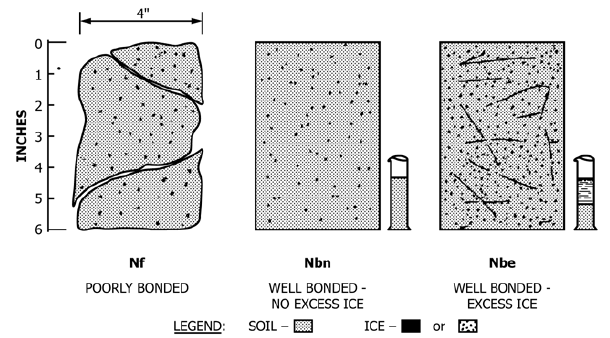
\includegraphics[width=0.6\textwidth]{part1_klass}
\caption{Illustration af de tre kategorier \textbf{Nf},\textbf{Nbn} samt \textbf{Nbe} (ASTM,2007).}
\label{fig:del2_klass}
\end{figure}
%

Prøver der klassifiseres som V deles ind i fem undergrupper- Vx, Vc, Vr, Vs og Vu. Hvor Vx - indikerer individuelle is krystaller eller iklusioner. Vc - indikerer at is fremtreder som belægning på partiklerne. Vr - isformationerne er orienteret tilfældigt eller irregulært. Vs - isformationerne er stratificeret eller tydelig orienteret. Vu - isen er ensartet fordelt, se figur . 
%
\begin{figure}
\centering
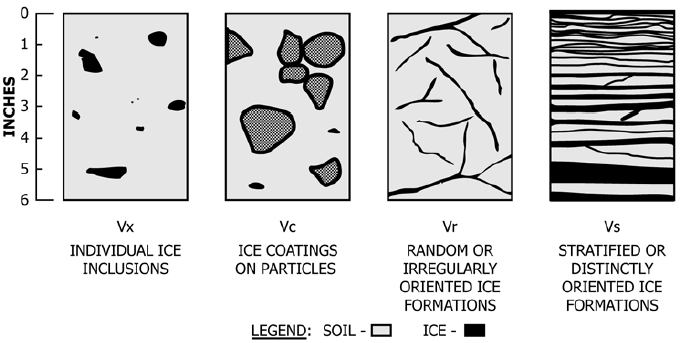
\includegraphics[width=0.6\textwidth]{part1_2_klass}
\caption{Illustration af de fire af de fem underkategorier for prøvens tilstand \textbf{Vx},\textbf{Vc} samt \textbf{Vr} og \textbf{Vs} (ASTM,2007).}
\label{fig:del2_klass}
\end{figure}
%
\subsection{Del tre}
Hvis isstrataen er tykkere en 25 mm som ICE, som deles op i to undergrupper ICE + Soil Type, hvis isinklusionerne indeholder jord og hvis istrataen ikke indeholder jord bliver den tildelt symbolet ICE. 
%%%%%%%

\section{Fotogrammetri- Struktureret lys}
\FloatBlock
Til 3D scanning af prøveemnerne er der anvendt HP 3D Struktureret lys skanner Pro SLS 3, med stereo kamera og rotationsbord.

\noindent Prøverne der scannes er forudbestemt, og er de samme prøver som ved klassifikationen. 
3D scaneren opstilles og kalibreres som beskrevet i bilag \vref{app:3dscan_vejledning}.

% Før prøverne scannes, vejes prøverne tre gange, derefter centreres prøven på rotationsbordet, lys og fokus stilles på kameraerne, se figur \vref{fig:sls_opstilling}. Derefter flyttes prøven og kalibreringspanelet placeres hvor prøven stod \todo[inline,backgroundcolor=anders]{sett inn bilde av kalibreringspanelet}. Ved kalibrering kan det være nødvendig at justere lukketid på de to kameraer samt fokus på både kamera og projektor, dette klaser fra software.

% Efter kalibrering, stilles prøven tilbage, lukketid og fokus stilles, derefter startes scanningen. 
\noindent For skanningen er der valgt tre forskellige rotationsvinkler, se tabel \vref{tab:antal_scans}. Rotationsbordet drejer prøven det valgte antal grader mellem hvert scan. Efter en fuldstendig  360$^{\circ}$ skan, vendes prøven på hovedet og scannes på nyt. Før scanning renses prøven for løst materiale, dette gøres i hånden, derefter vejes prøvens masse. Denne proces gentages inden hver enkelt scanning.

Alle prøver scannes tre gange ved en rotationsvinkel på 45$^{\circ}$. Rotationsvinkelens indflydelse på den beregnede bulkdensitet undersøges ved at fire prøver, scannes tre gange ved rotationsvinkel på 60$^{\circ}$ samt 72$^{\circ}$. De fire prøver der skannes ved 60$^{\circ}$ og 72$^{\circ}$ ses i tabel \vref{tab:prover_60_72}.  
%
\begin{table}
\centering
\topcaption{Rotationsvinkel, og antal skans på 360\degree}
\label{tab:antal_scans}
\begin{tabular}{cc}
\textbf{Vinkel[\degree]} & \textbf{Antal scans}	\\	
\toprule
45	&	8		\\
60	&	6		\\
72	&	5		\\
\bottomrule
\end{tabular}
\end{table}
%
\begin{table}
\centering
\topcaption{Prøve, rotationsvinkel}
\label{tab:prover_60_72}
\begin{tabular}{lcc}
\textbf{Prøve} & \textbf{Grader [\degree]} \\	
\toprule
 B16002\_5B & $60$ & $72$ \\
 B16004\_3F & $60$ & $72$ \\
 B16012\_7D & $60$ & $72$\\
 B16019T\_8F & $60$ & $72$ \\
\bottomrule
\end{tabular}
\end{table}
%

Når alle prøver er scannet en gang (top+bund), ved den givne rotationsvinkel, kalibreres scanneren på nyt og prøverne scannes igen ved samme metode som tidligere angivet. 
Udover de givne 15 prøver er der lavet tre referenceemner, en terning og to cylindre, for terning se figur \vref{fig:terning}, for cylinder 1 se figur \vref{fig:cylinder_1} og for cylinder 2 se figur\vref{fig:cylinder}. De tre referenceemner er scannet for at give et en forståelse af scannerens nøjagtighed. De tre objekters dimensioner målet tre gange med et elektronisk skydelær med en opløsning på 1/10 millimeter. 
Derefter scannes referenceobjekter, tre gange ved en rotationsvinkel på 45$^{\circ}$. Oprindeligt var prøverne hvide, dog var overfladen for blank til at struktureret lys kan anvendes, de ble derfor overfladebehandlet med mat-zinkspray, se figur \vref{fig:zink_spray}.
%
\begin{figure}
\centering
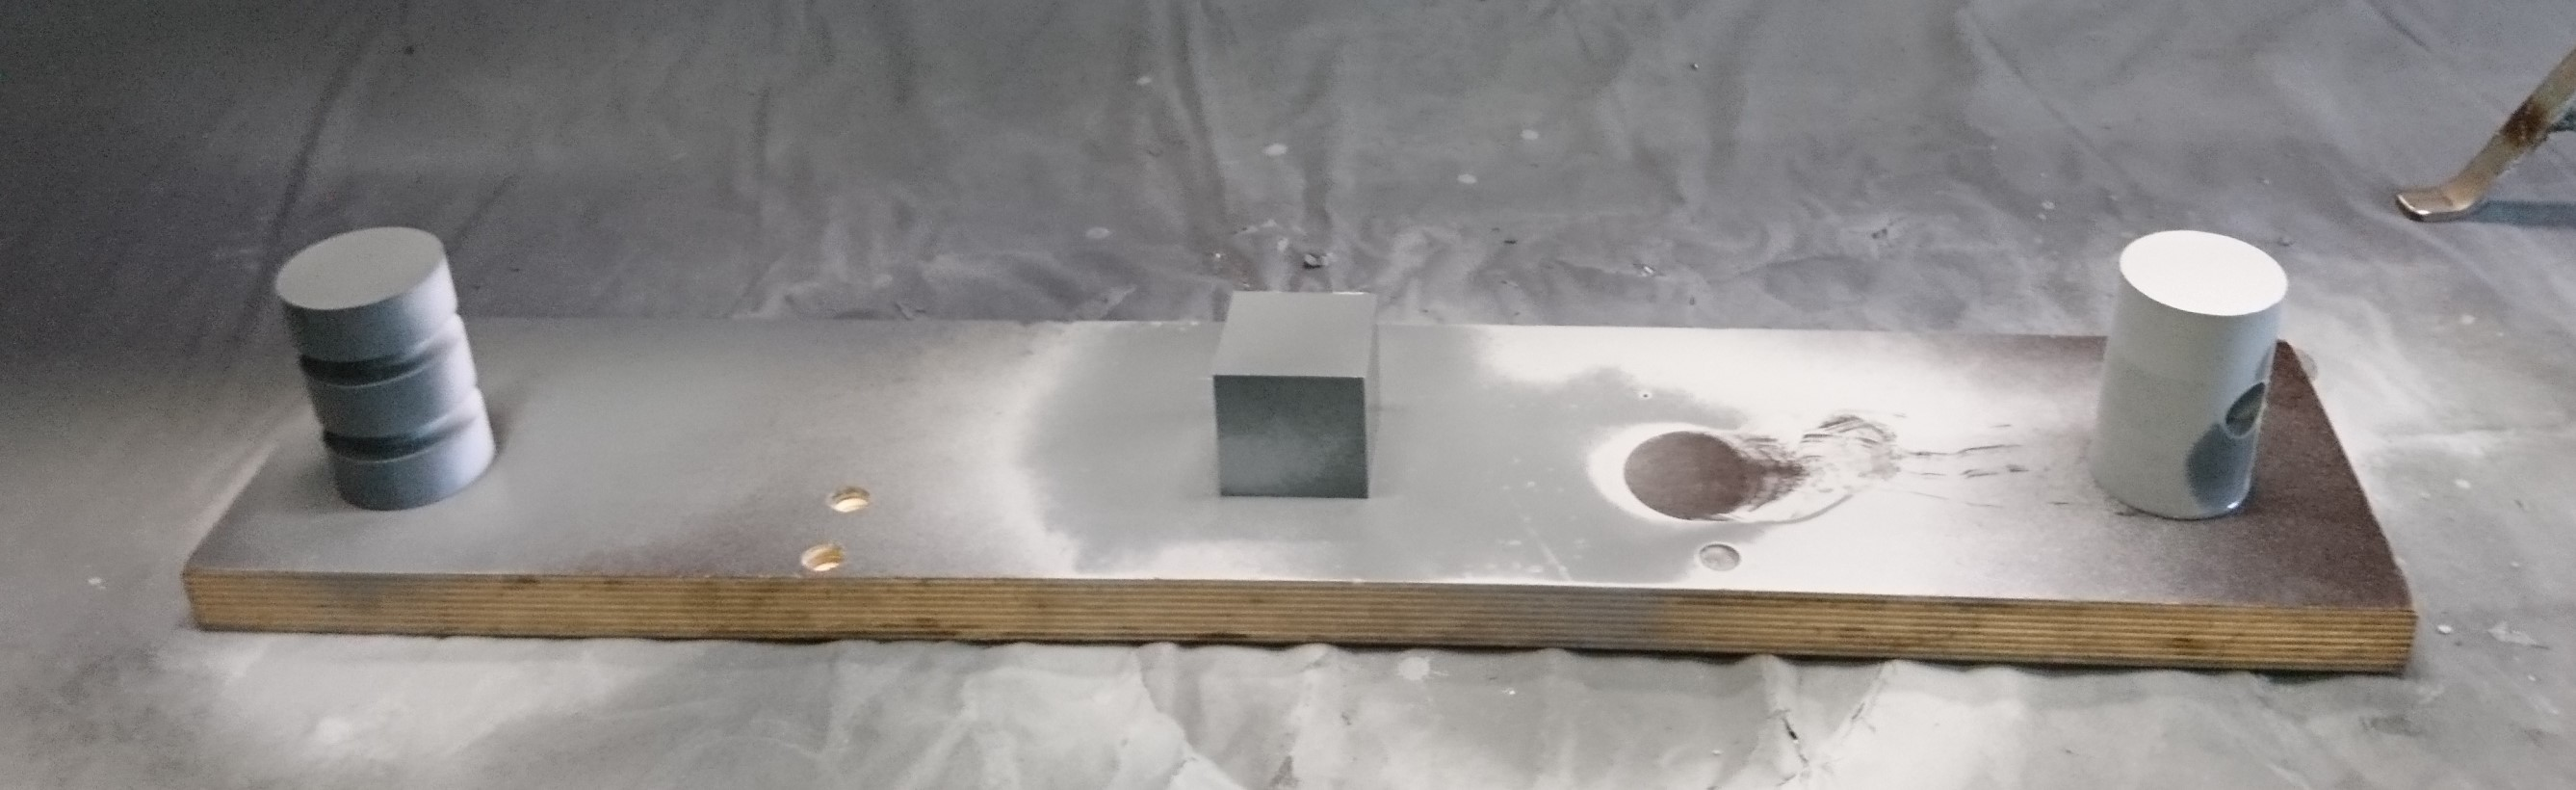
\includegraphics[width=0.6\textwidth]{ref_emner_spray}
\caption{Referenceemnerne gives en mat overflade, med zink spray}
\label{fig:zink_spray}
\end{figure}
%
%
 \begin{figure}
 \centering
 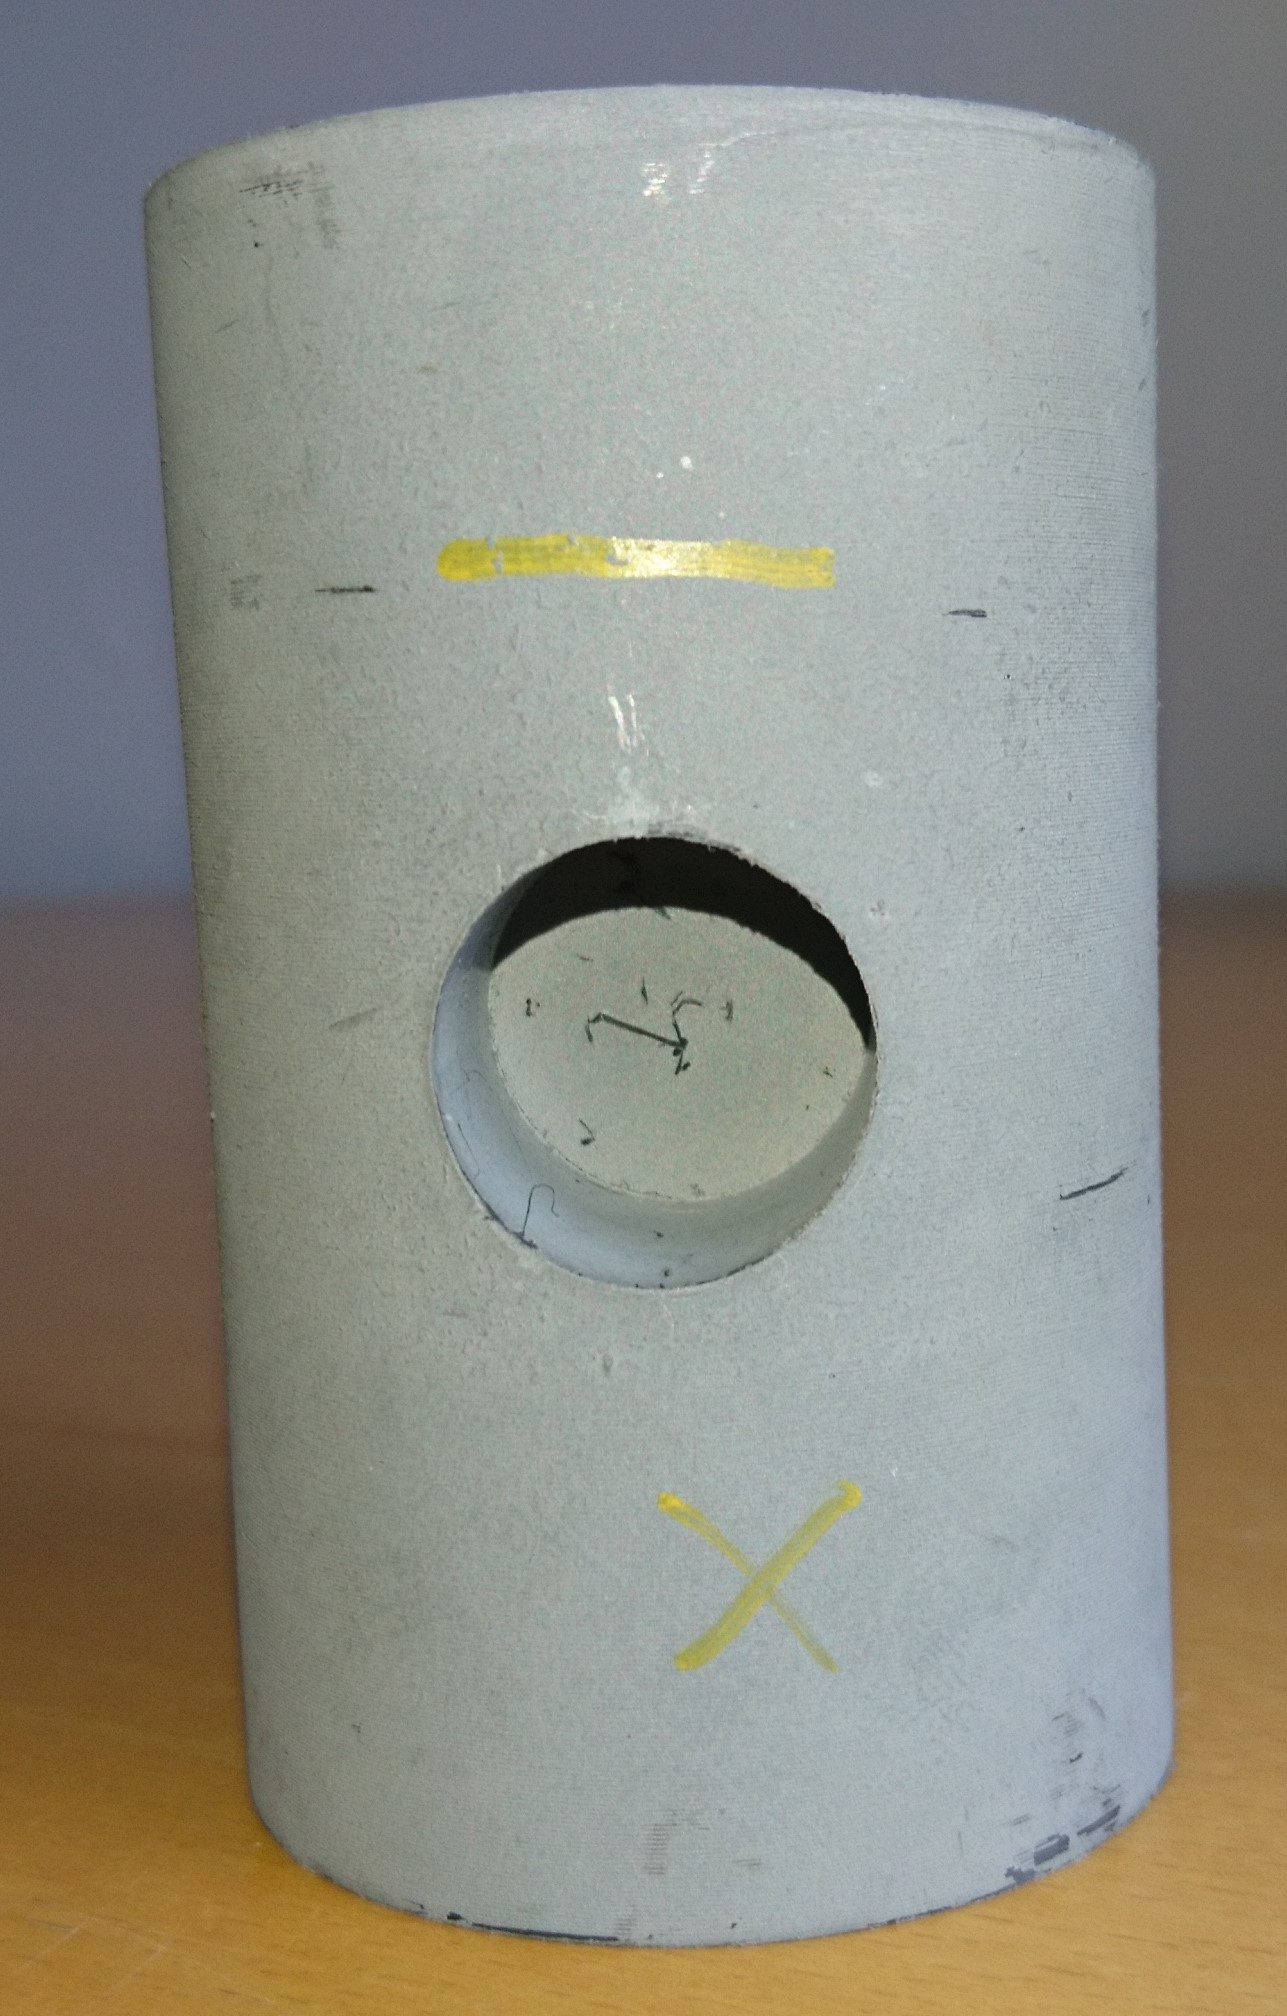
\includegraphics[width=0.3\textwidth]{cylinder_1}
 \caption{Referenceemne - cylinder 1 med dyb indsænkning}
 \label{fig:cylinder_1}
 \end{figure}
%

%
\begin{figure}
\centering
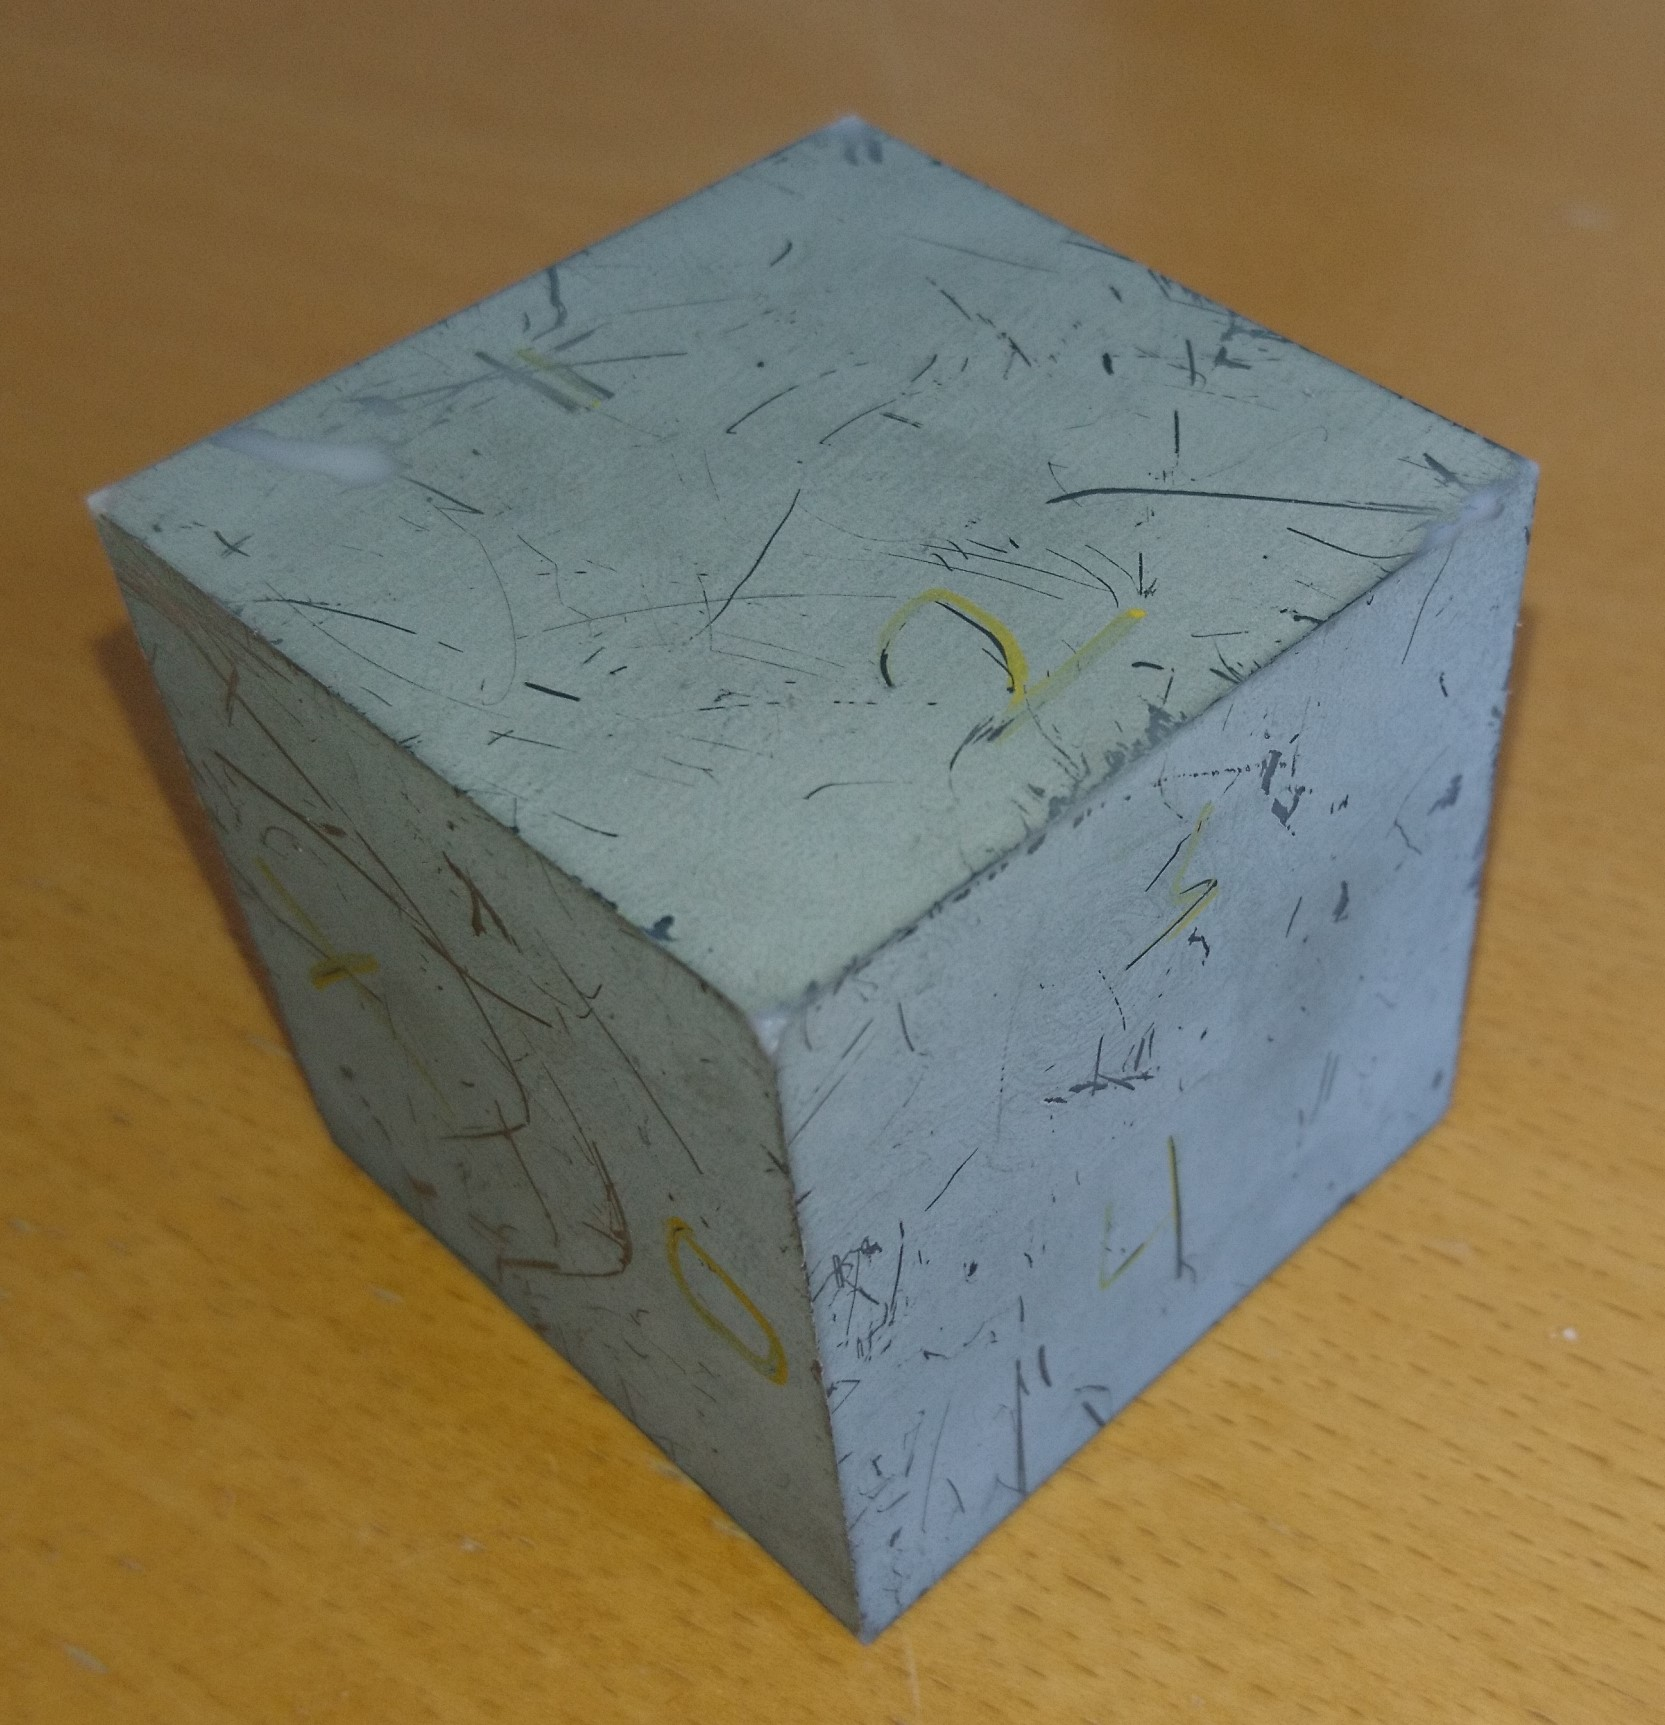
\includegraphics[width=0.4\textwidth]{terning}
\caption{Referenceemne - terning}
\label{fig:terning}
\end{figure}
%
%
\begin{figure}
        \begin{subfigure}[b]{0.45\textwidth}
                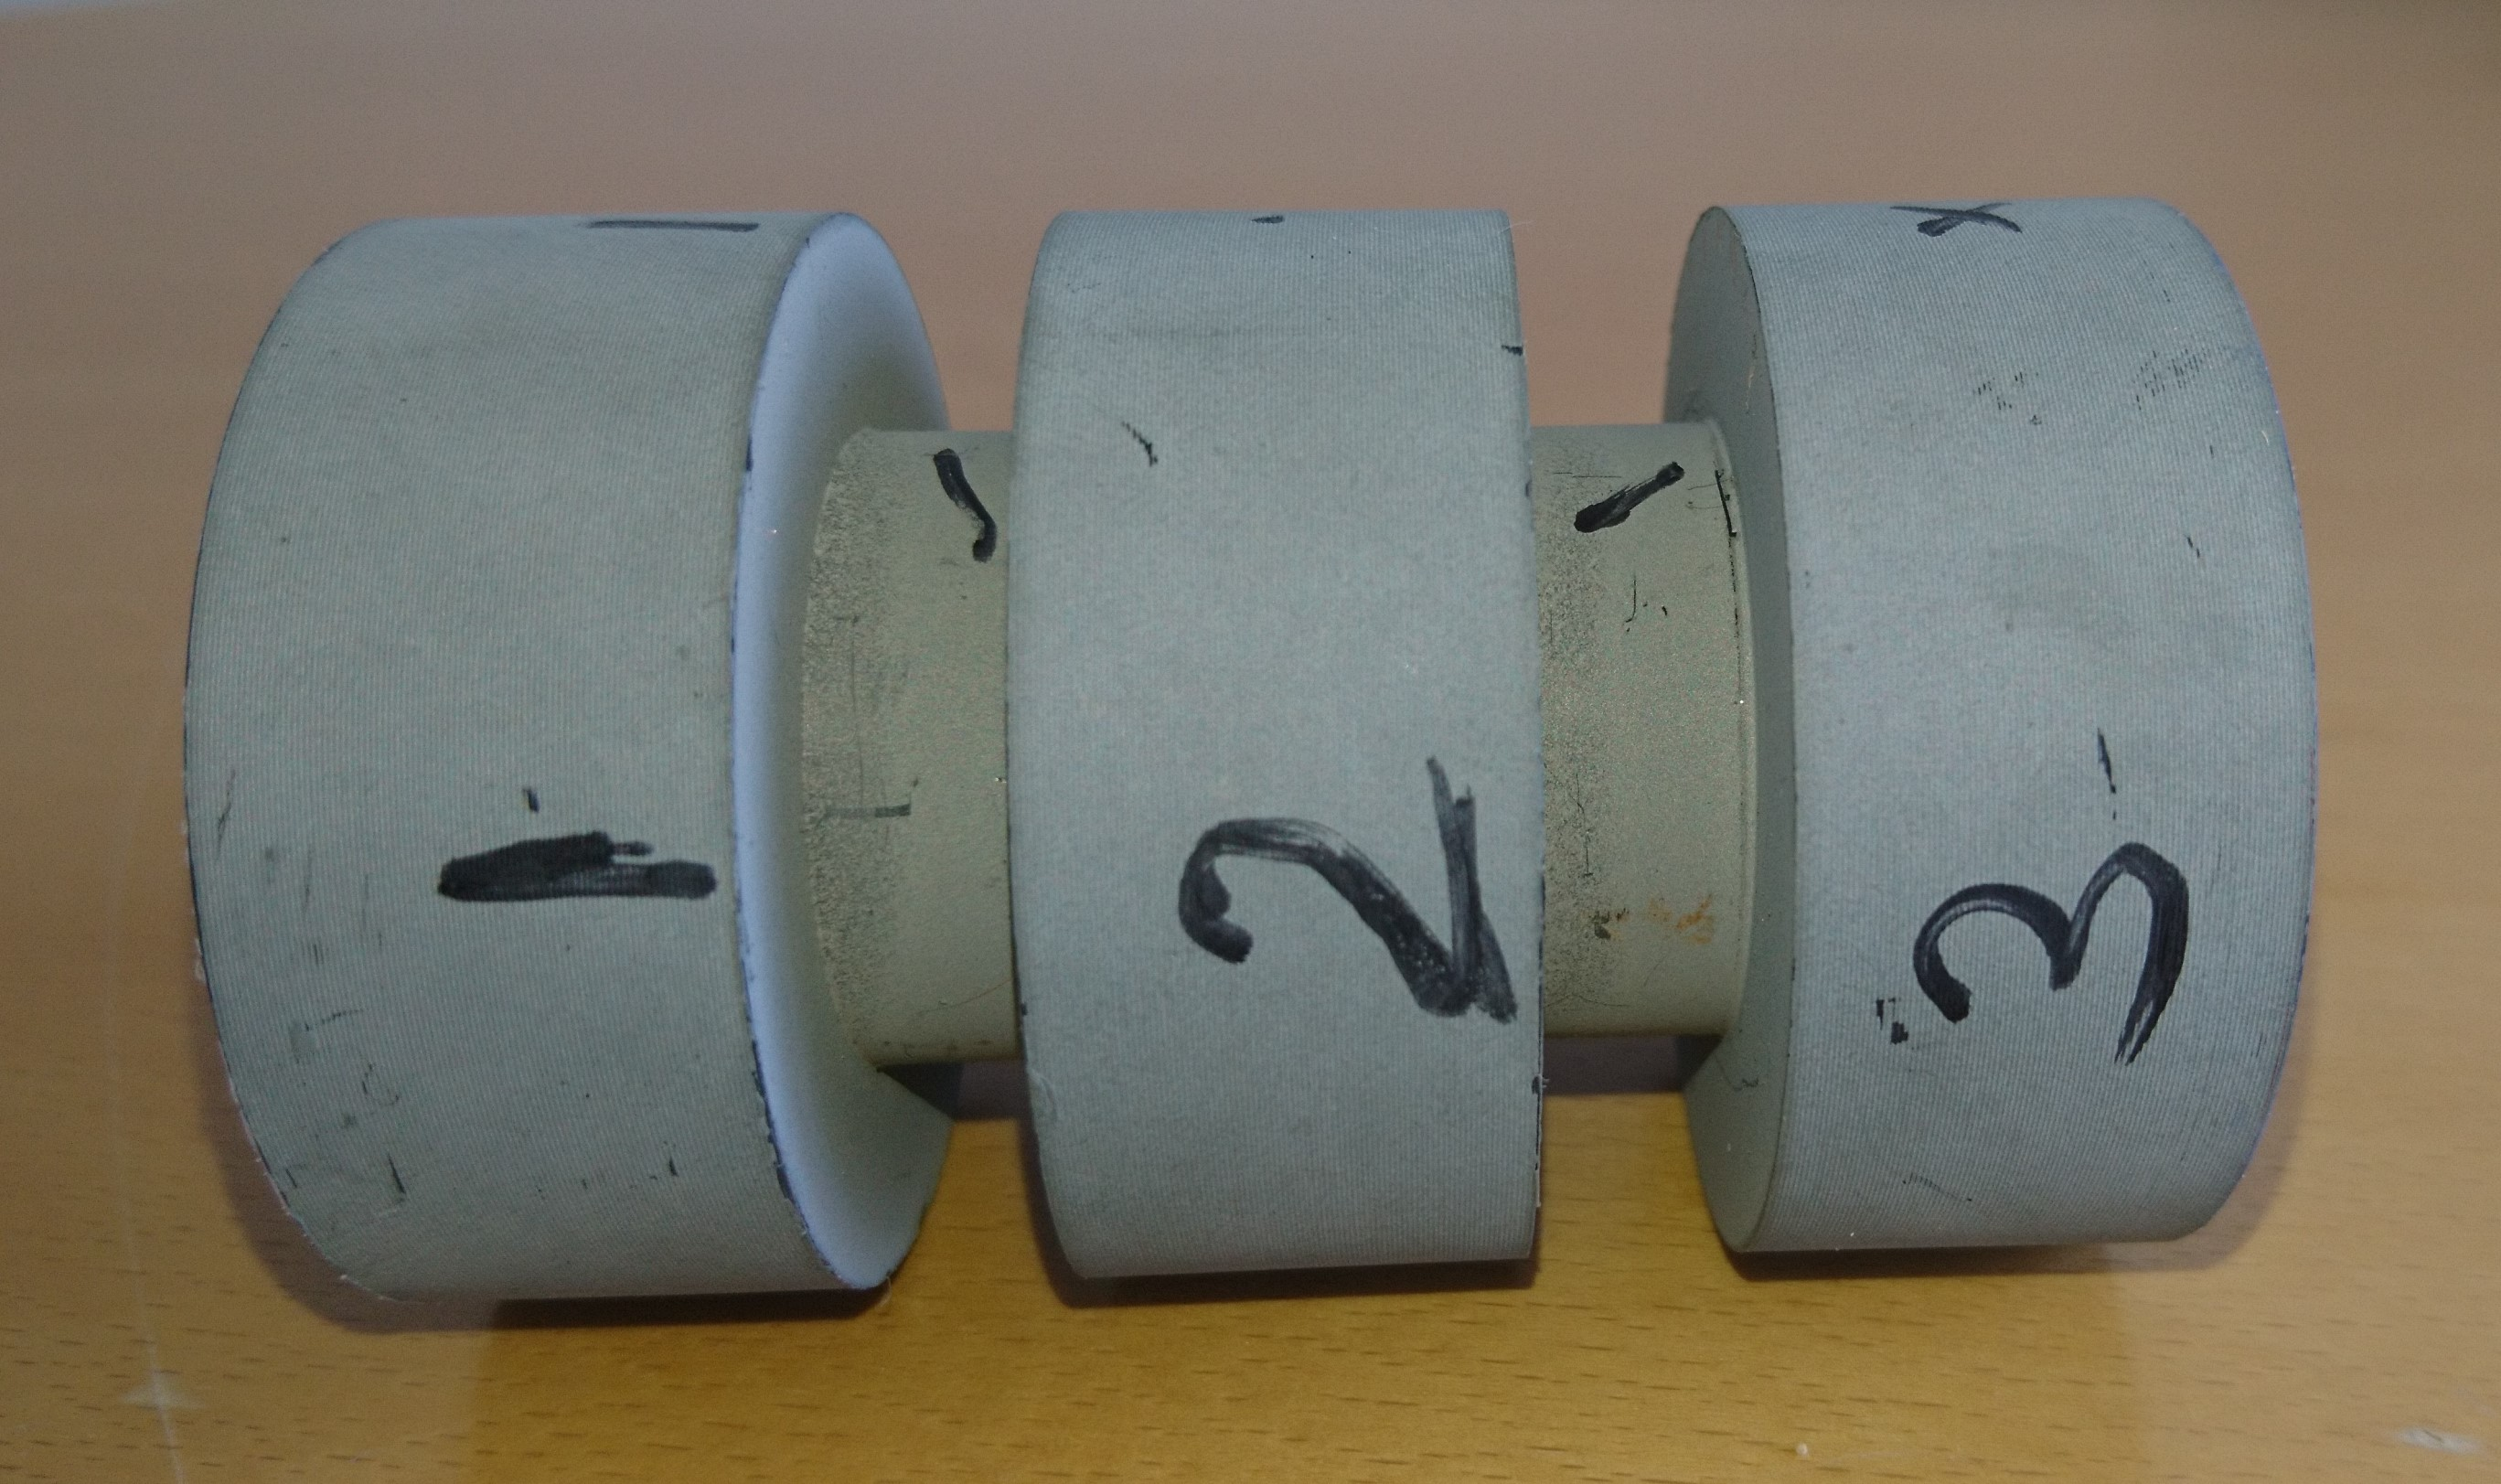
\includegraphics[width=\linewidth]{cylinder_2_2}
                \caption{Cylinder 2 liggende}
                \label{fig:cylinder 2 liggende}
        \end{subfigure}\hfill %
        \begin{subfigure}[b]{0.40\textwidth}
                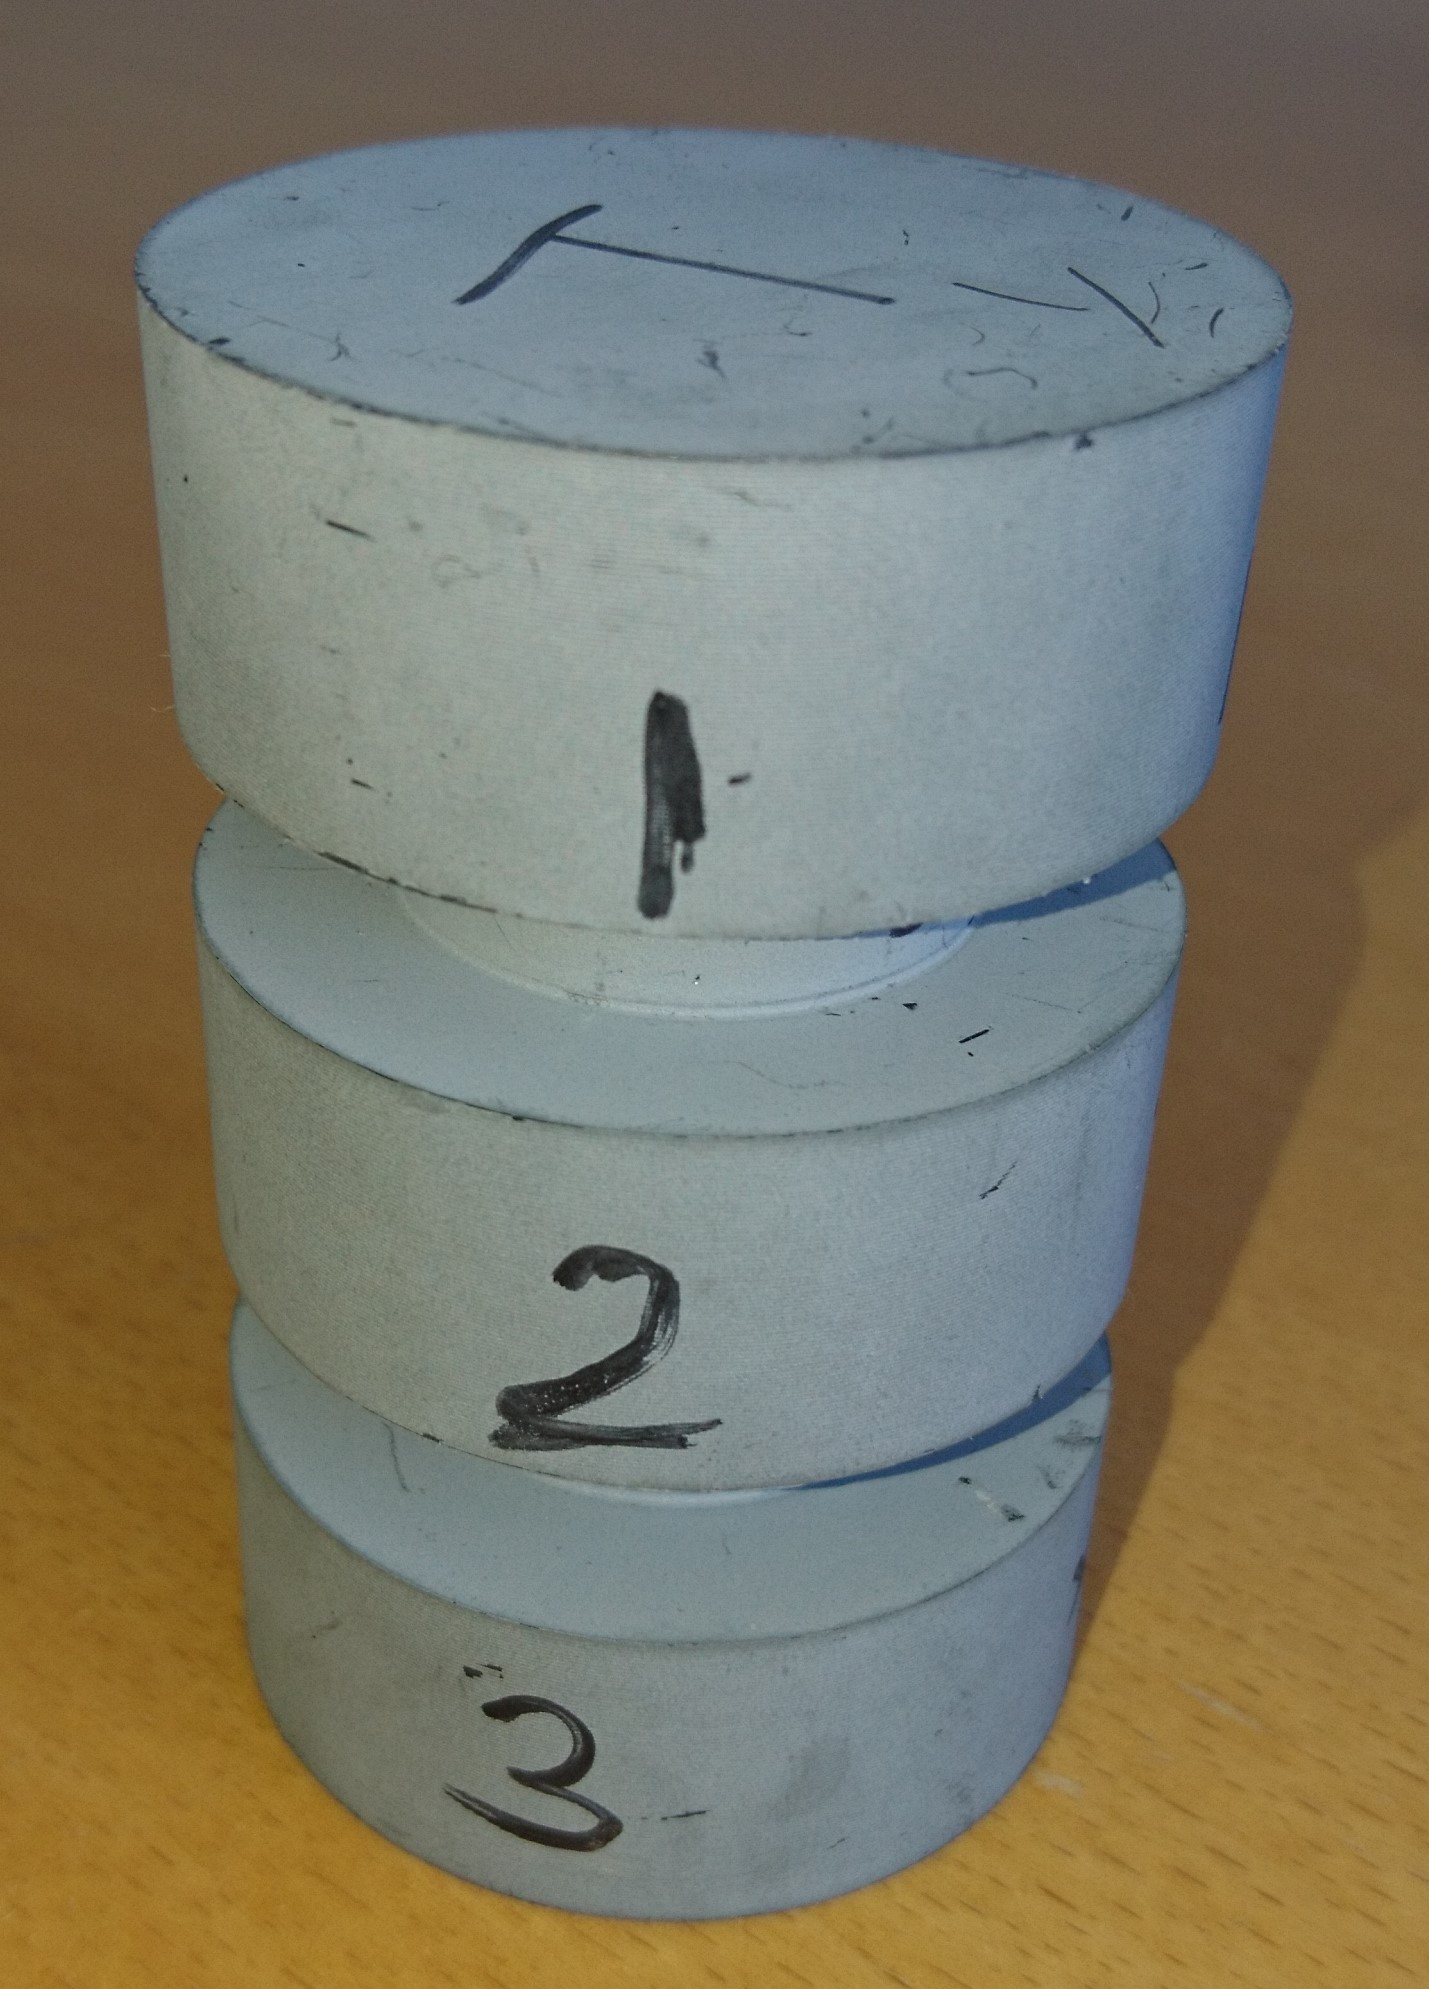
\includegraphics[width=\linewidth]{cylinder_2_3}
                \caption{Cylinder 2 stående}
                \label{fig:cylinder2}
        \end{subfigure}%
        \caption{Referenceemne - cylinder med udfræsninger}\label{fig:cylinder}
\end{figure}
%

Udførelsen af 3D scanning har foregået i frostrummet på DTU, Lyngby, for opstilling se figur \vref{fig:sls_opstilling}. 
%
\begin{figure}
\centering
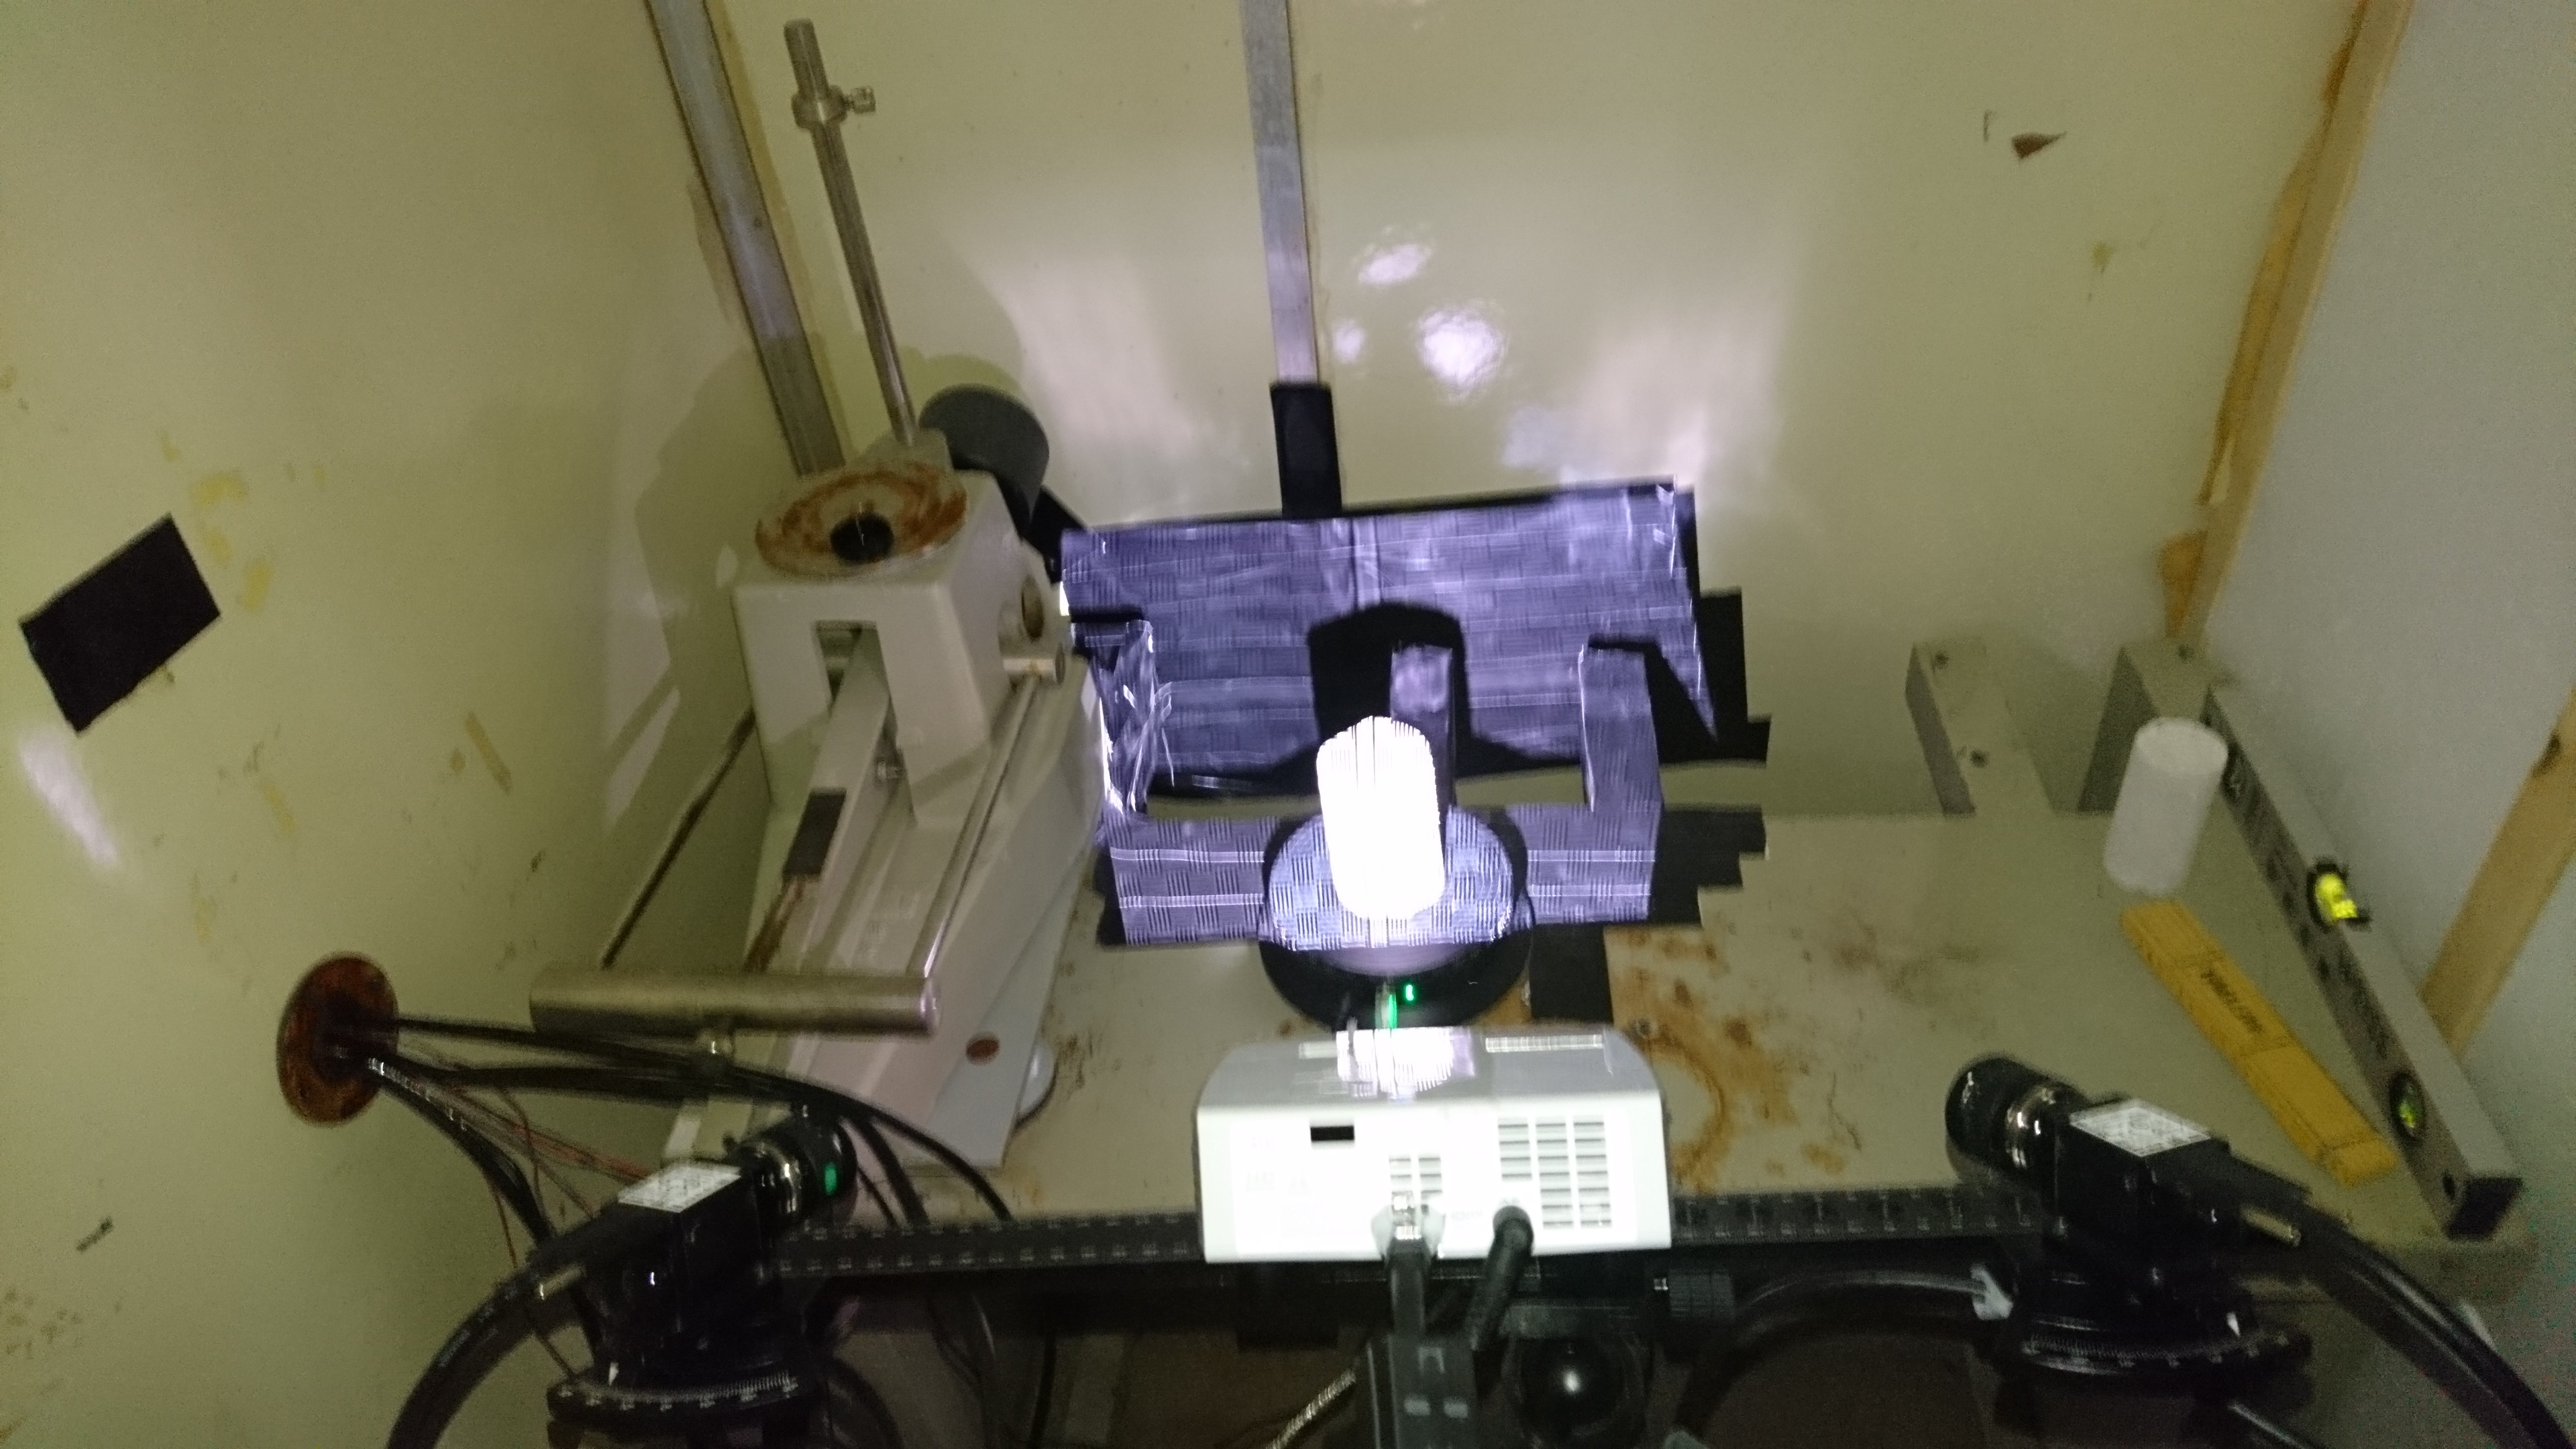
\includegraphics[width=0.7\textwidth]{opstilling_sls_red}
\caption{Prøveopstilling, struktureret lys}
\label{fig:sls_opstilling}
\end{figure}
%

%
%
\noindent Efter alle prøver er scannet, efterbehandles den indsamlede data, som beskrevet i vejledningen se bilag \vref{app:3dscan_vejledning}, og der dannes et vandtæt mesh. 
%
\paragraph{Volumen af mesh} bliver beregnet af to programmer, HP 3D scan og Python. HP 3D scan programmet haver en indebyget funktion der angiver volumen. Til sammenligning er der anvendt Python-modul der kalkulerer volumen af den vandtætte overflade fra stl-fil, til volumen beregning med python anvendes script i separat vedhæftet fil "volumen\_3dscan.py".

\paragraph{Beregning af usikkerhed}
Da de tre scanninger af en prøve er uafhængige af hinanden, masse og volumen kan ændres i mellem hver scanning (m1,m2,m3,v1,v2,v3), bliver m1,v1 osv. parret, og resultatet angives derfor som en middelværdi $\pm$ en spredning. 
Der tages kun højde for den variation der er i densitetsmålingerne, fejlkilder som kan bidrage er vægten, kalibrering af scanner, hvor godt den endelige model passer med punktskyen samt hvordan volumenet beregnes. 
% Til sidst laves der en 3D pdf fremstilling af de 15 prøver der er skannet ved rotationsvinkelen 45$^{\circ}$, samt referenceobjekterne, dette gøres ved at konvertere meshet fra stl- til u3d- format i MeshLab, se separat fil \todo[inline,backgroundcolor=anders]{sett ind navnet på filen}. 
%
\paragraph{Afvigelser fra vejledning:} ved efterbehandling af data blev det konstateret at flere af reference scanningerne ikke var gode nok, pga. den begrensede tidperiode projektet løber over, har der ikke været tid til at lave nye scans af reference emnerne. For at kunne scanne hele fordybningen i cylinder 1 var det nødvendigt at lægge cylinderen vandræt på rotationsbordet, dette medførte problemer ved efterbehandlingen, og det lykkedes ikke at sætte de forskellige scans sammen, af denne grund er forkastes scans og modeller af cylinder 1 og indgår ikke i den videre efterbehandling af resultater. For de to andre referenceemner terning og cylinder 2 kunne der ses i efterbehandlingen at allignment processen ikke blev optimal for de to scanninger, terning 1 og cylinder 2\_1. De har dog blevet vurderet til at være gode nok til den videre efterbehandling.

%%% ---------- Arkimedes princip ---------- %%%
\FloatBlock
\section{Arkimedes princip}
Til den anden del af volumen bestemmelse anvendes Arkimedes princip, hvor prøven neddykkes i en blanding af paraffin og olie (Isopar- L), se datablad i bilag \vref{app:data_isopar}.
Isopar anvendes da forsøget udføres ved en temperatur på $-6${\celsius}.  

\noindent En beholder med Isopar stilles ovenpå en vægte, en separat prøveholder henges op, så den hverken prøveholder eller prøve berører Isopar-beholderens bund eller sider. På prøveholderen festes en temperatur føler. I det følgende anvendes følgende notation: Isopar- I, prøveholder H, vægt/lod - V og prøve - P.

Densiteten af Isopar-L er afhængig af temperaturen, af denne grund bestemmes densiteten af Isopar ved målinger af et lod med et kendt volumen og masse. 

\subsection{Kalibrering af temperaturfølere}
Til måling af temperatur (luft og Isopar) anvendes der datalogger med en opløsning på $0,1${\celsius}. Det anvendte kalibreringsbad til nulpunktskalibrering  er " Fluke 7320" se figur \vref{fig:kalibad}. De tre temperatursensorer festes til metal gitteret, og nedsænkes i kalibrerings-badet. Inden forsøgsstart kalibreres temperaturlogger med computer tid (tt:mm:ss), armbåndsuret til at notere tidspunkt for hver måling inde i frostrummet kalibreres efter computeren.

%
\begin{figure}
\centering
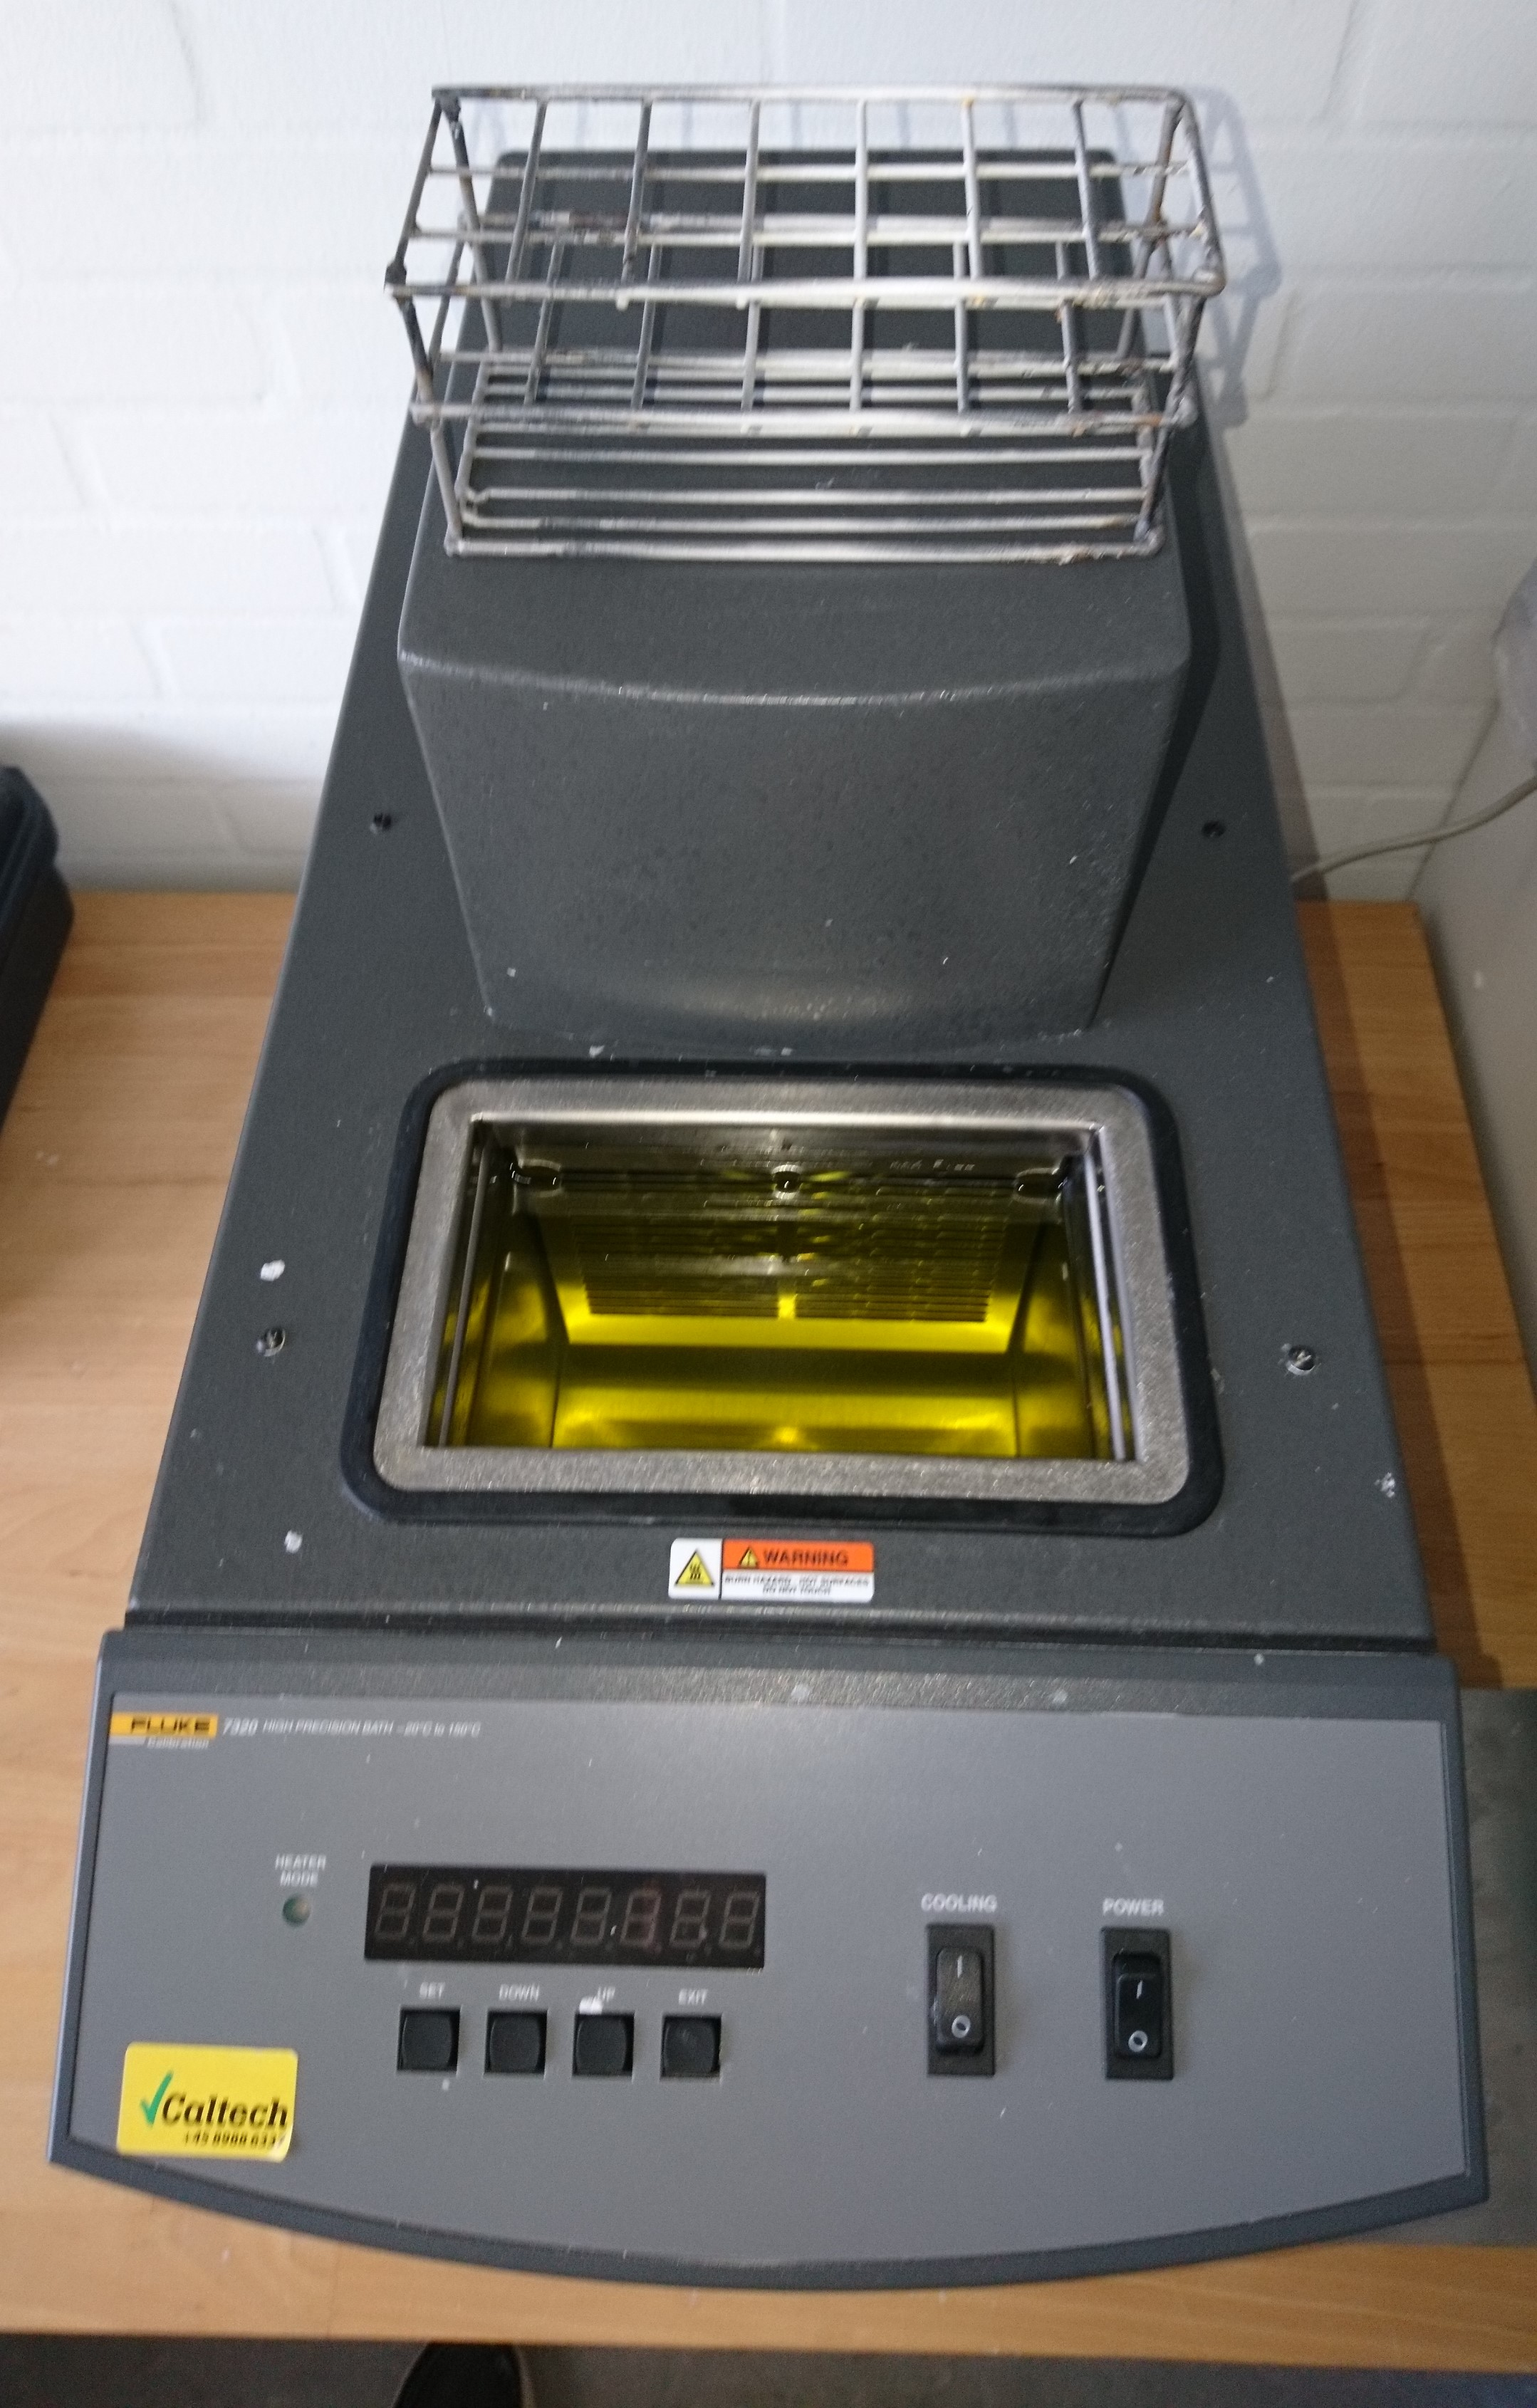
\includegraphics[width=0.3\textwidth]{kalibrerings_bad}
\caption{Det anvendte kalibreringsbad}
\label{fig:kalibad}
\end{figure}
%

Som udgangspunkt for nulpunkts kalibreringen er er "Fluke Termometer 1524" benyttet med den tynde/fleksible termistor probe. Den fejl der er på de to følere, legges til/ trækkes fra temperaturen i forsøget under resultatbehandling.
For at sikre mindst mulig forstyrrelse er dataloggeren sat til at starte målingerne efter computeren er koblet fra. For reference termometret er strømforsyningen valgt fra da den giver forstyrrelser og der er i stedet benyttet batterier.

\subsection{Forsøgsgang}
For alle målinger noteres temperatur og vægt [g], inden forsøgsstart renskes prøverne for evt. løst materiale, hvilket gøres for hånd. Derefter vejes prøven tre gange.

Vægten af isopar noteres, vægten nulstilles. Prøveholderen kommes i, derefter kommes loddet i (I+H+V), denne process (I+H,I+H+V), gentages to gange. 
Prøven kommes i, efter masse og tid er noteret tages prøven op og tørres af med papirservietter, derefter kommes holderen i, dette gentages tre gange for hvert prøveemne (I+H,I+H+P,I+H).
Efter prøven er neddykket tre gange afsluttes denne sekvens ved følgende målinger: I,I+H,I+H+V. Når en sekvens er fuldføret (en prøve) kan næste sekvens starte (prøve 2) hvor samme procedure følger. Når alle prøver er kommet i tre gange, afsluttes forsøget ved: I,I+H,I+V+H,I+H,I+V+H. For en skematisk oversigt over proceduren henvises der til bilag \vref{app:skema_ark}.

\subsection{Beregning af densitet} 
Temperatur logger og tidspunkt for målinger samkøres på den fælles tid. 
Derefter beregnes $\rho_iso$ for alle målinger med loddet, se formel 

Densiteten af Isoparens bestemmes ved at sænke et lod med kendt masse og kendt volumen ned i beholderen med Isopar, hvilket gøres to gange ved forsøgs-start og to gange ved forsøgs-slut. Hver prøve neddykkes tre gange, hvor der forinden og efter de enkelte neddykk, noteres vægten af isopar + holder. Temperaturen ved hver nedsænkning noteres, og anvednes til at samkøre temperaturmålingerne fra datalogger med de enkelte neddykkninger

Ved Arkimedes princip kan et objekts volumen bestemmes, dette gøres ved at nedsænke et legeme i en væske. Den opadrettede kraft $F_op$ (opdriften) som påvirker legeme, svarer til massen af den fortrængte væske.

Til bestemmelse af Isoparens densitet, nedsænkes et legeme med kendt masse og volumen, hvor forskellen i massen $\Delta_m$, før og efter legeme nedsænkes, svarer til volumen af det neddykkede objekt. Væskens densitet $\rho_{liq}$ bestemmes ved følgende formel \vref{eq:rho_iso}, hvor $\delta_m$ er forskellen i den noterete vægt, og $V_{obj}$ er volumen af loddet.     

%
\begin{equation}
\label{eq:rho_iso}
\rho_{I}=\frac{\Delta{_m}}{V_{obj}}  
\end{equation}
% 

De målte densiteter af isopar plottes som en funktion af den målte temperatur, og der etableres en lineær regressions linje, ud fra regressions linjens formel findes densiteten af isopar ved de målte temperaturer. 

Volumen af de enkelte prøver $V_P$ beregnes ved formel \vref{eq:vol_prove}, hvor $\Delta{m_p}$ er forskellen i den noterte vægt og $\rho_I$ er den beregnede densitet for isopar, ved den aktuelle måling.

%
\begin{equation}
\label{eq:vol_prove}
V_p=\frac{\Delta{m_p}}{\rho_I}
\end{equation}
%

%
\begin{figure}
\centering
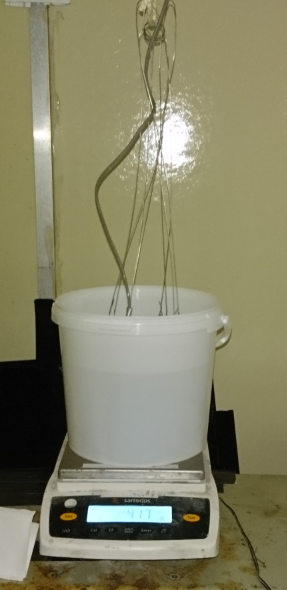
\includegraphics[width=0.30\textwidth]{ark_opst_red}
\caption{Forsøgs opstilling- Arkimedes princip}
\label{fig:ark_opst}
\end{figure}
%
\begin{figure}
\centering
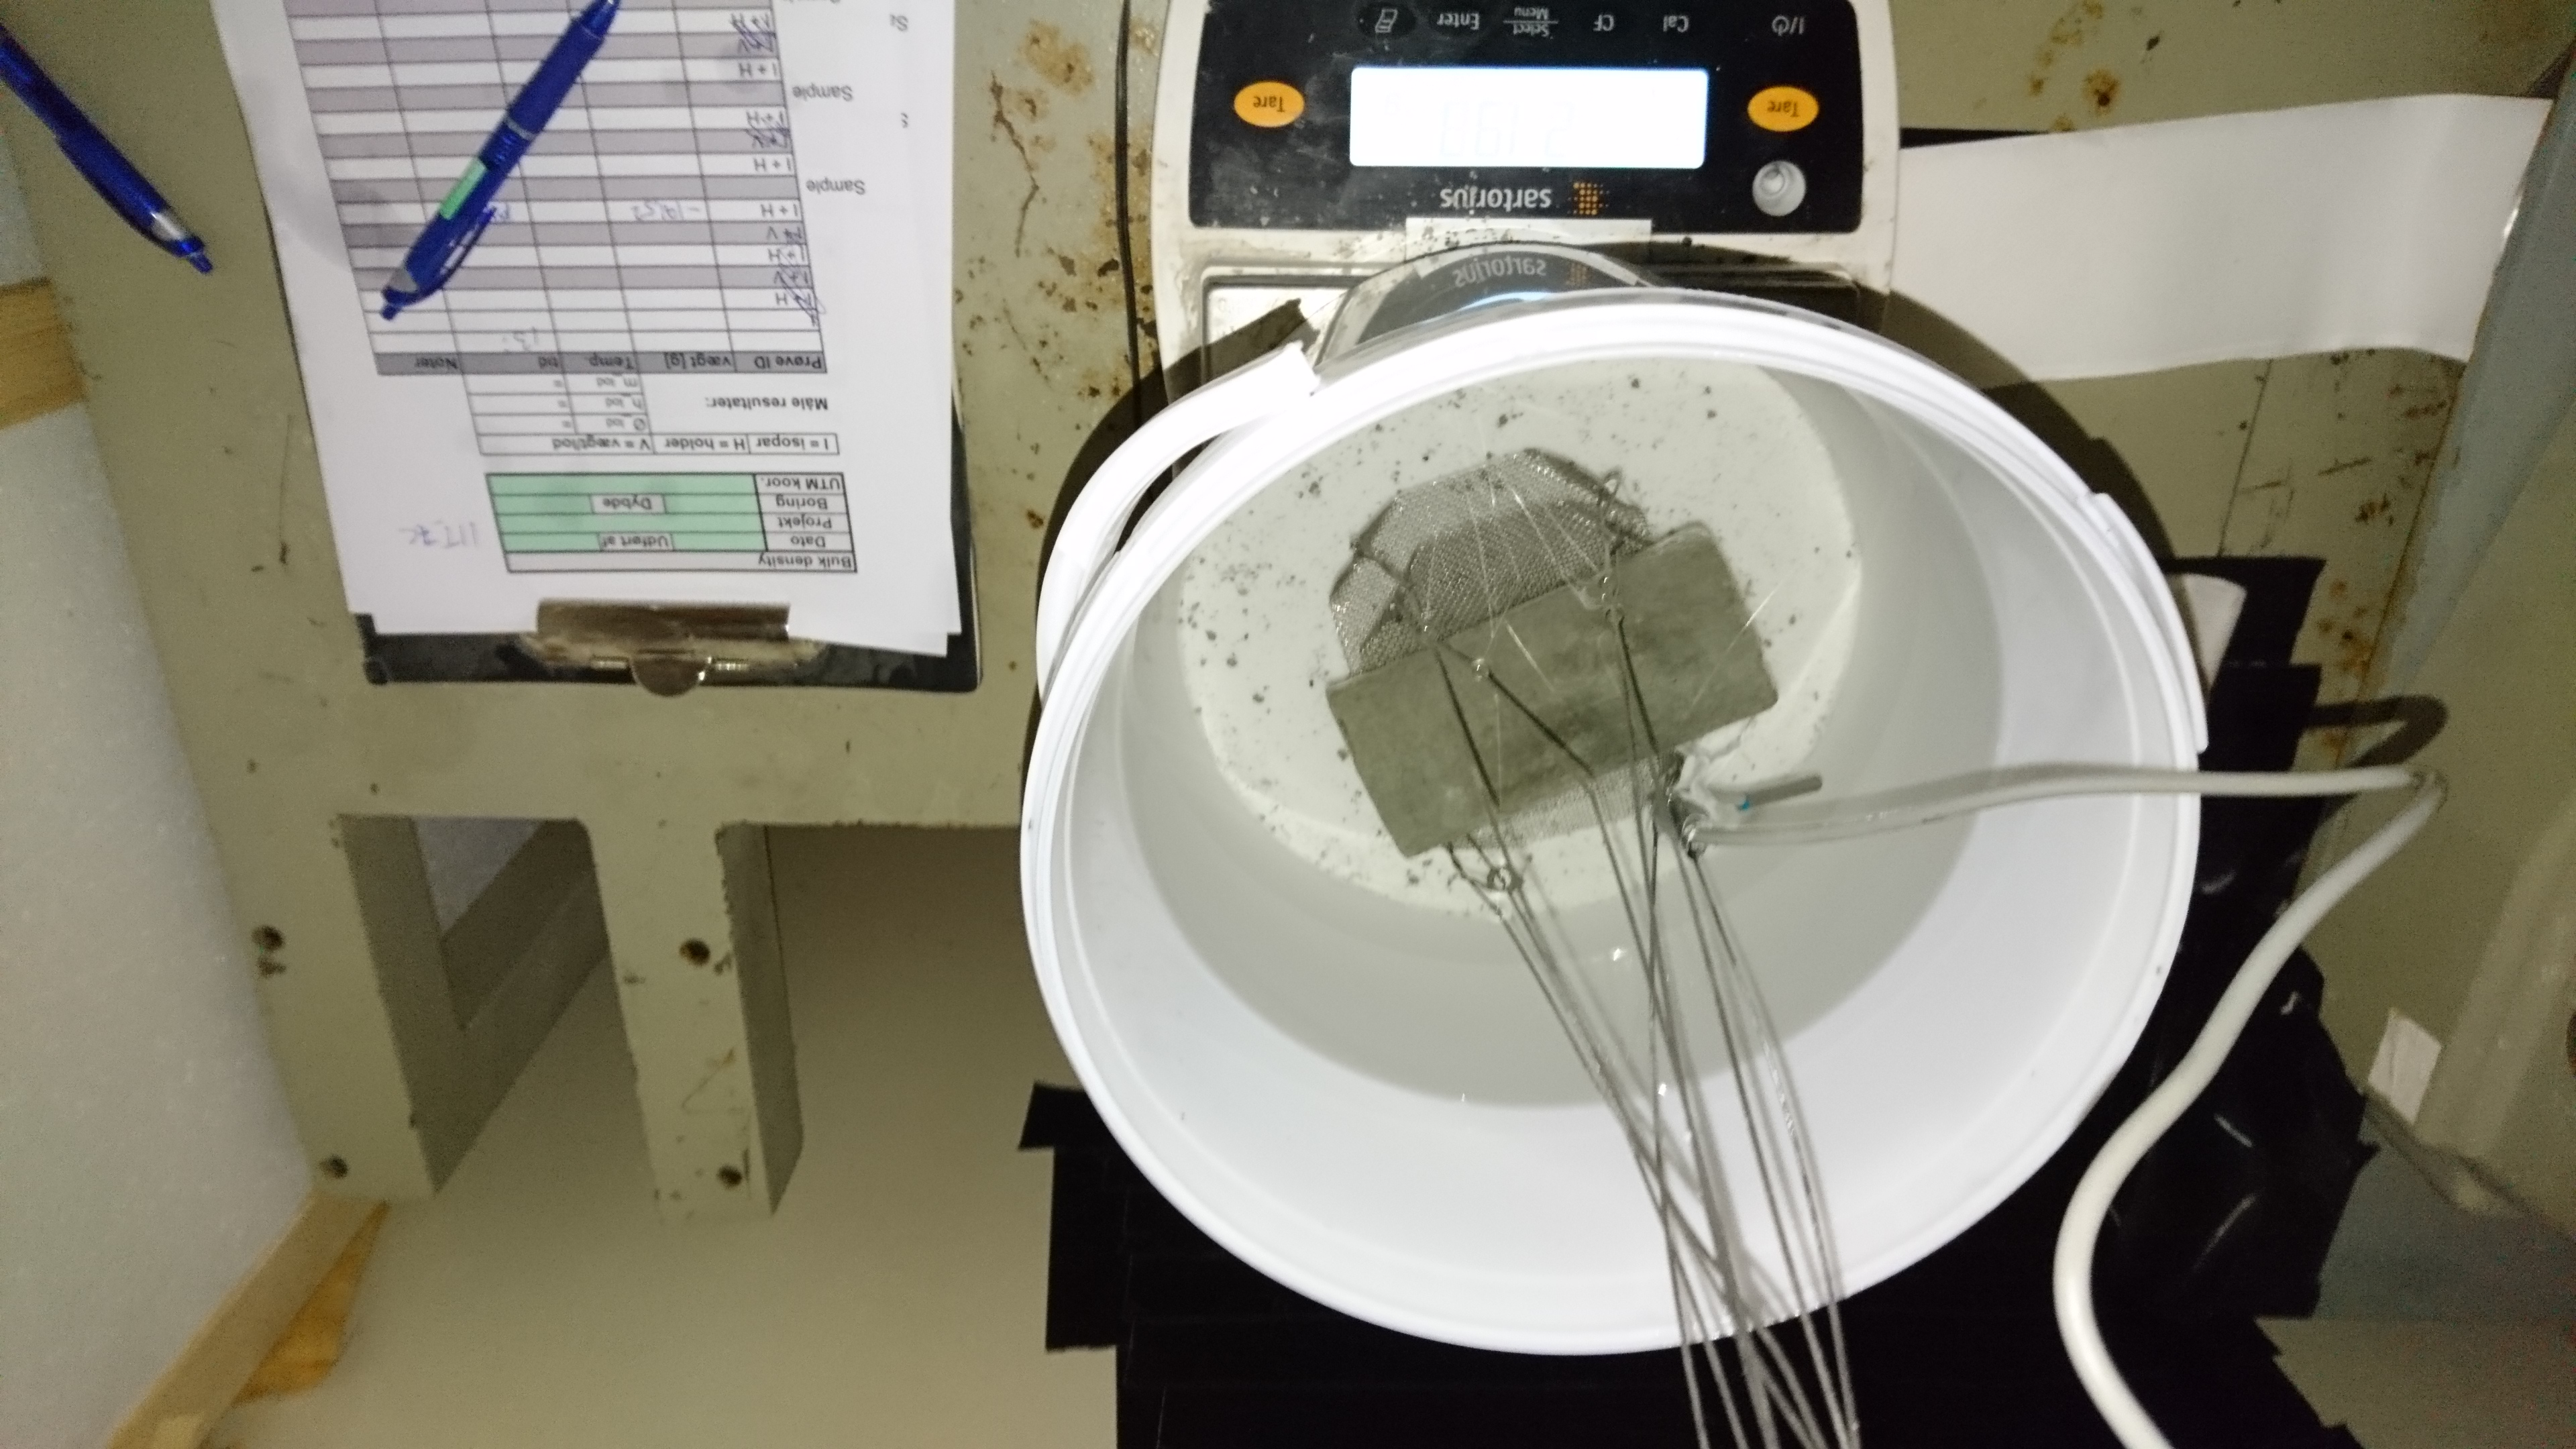
\includegraphics[angle=180,width=0.55\textwidth]{ark_prove}
\caption{Forsøgs opstilling, med prøve neddykket i Isopar}
\label{fig:ark_opst_prove}
\end{figure}
%
\paragraph{Beregning af usikkerhed}
Til bestemmelse af densiteten af isopar ved hvert enkel prøveemne anvendes en middelværdi af densiteten bestemt inden prøven nedsænkes i væsken samt den efterfølgende densitets bestemmelse. Ud gennemsnits densiteten for isopar beregnes tre volumener. Gennemsnits volumen og gennemsnits massen anvendes til at beregne bulkdensitet af prøven, ved formel \vref{eq:sd_dens}. 
%
\begin{equation}
\label{eq:sd_dens}
\frac{\sigma_\rho}{\bar{\rho}}=\sqrt[]{(\frac{\sigma_m}{\bar{m}})^2+(\frac{\sigma_v}{\bar{v}})^2}
\end{equation}
%
\paragraph{Afvigelser fra vejledning} Temperatur data fra nullpunktskalibreringen har ikke blevet behandlet, dette vil give en mindre fejl på temperaturen, isoparens densitet samt loddets volumen, dog vil det føre til en paralellforskyvning, da alle målinger vil flytte sig horisontalt langs x-axsen. Det er derfor valgt at benytte den gennemsnitlige densitet for isopar for hvert prøvemne som udgangspunkt for beregningerne, for isopars densitet plottet som funktion af temperaturen, henvises der til bilag .  så der vil ikke udgøre en forskel på beregningen af bulkdensiteten. 

\chapter{Resultater}
I dette afsnit bliver resultaterne for klasifikation, volumen beregninger samt densitet præsenteret. Volumenberegnignerne er lavet ved tre forskellige metoder der bliver holdt op mod hinanden. Fra struktureret lys er der beregnet volumen af permafrost kerner ved HP software samt et python-modul. De kalkulerede volumner fra scanningen, sammenholdes med volumen fra akrimedes princip.

\section{Visuel - klassifikation}
Den visuelle klassifikation er udført ihh. til standarden:AsTM D4083-89. Resultatet af den visuelle klassifikationen kan ses i tabel \vref{tab:klas_perma}. 
%
\begin{table}
  \centering
  \topcaption{Klassifikation af permafrostkerner, Prøve, Diameter på kerne, kernens dybde (meter under terreng), betegnelse og kommentar til kernen.}
  \label{tab:klas_perma}
  \begin{tabular}{l c l l l}
  \toprule
 \multicolumn{1}{l}{Prøve} & 	\multicolumn{1}{c}{Diameter$[cm]$} & \multicolumn{1}{l}{M.U.T} &	\multicolumn{1}{l}{Betegnelse} & \multicolumn{1}{l}{Kommentar} \\
\midrule
$B16001T\_6D$&	7&	2,90-3,00&	Is+ler&	Isen er klar og tåget\\
$B16002\_5B$&	7&	1,89-1,99&	Is+ler&	Isen er klar og tåget\\
$B16003\_8D$&	7&	4,65-4,75&	Nbe&	vel sammenhængende\\
$B16004\_3F$&	7&	1,30-1,40&	Is+Ler& Isen er klar og tåget\\
$B16005T\_6E$&	5&	2,62-2,72&	Vx&	Individuelle isinklusioner\\
$B16007\_7G$&	7&	2,60-2,70&	Vx&	Individuelle isinklusioner\\
$B16009T\_7G$&	7&	3,75-3,85&	Vs&	Horisontalt orienteret isformationer\\
$B16010T\_7G$&	7&	3,10-3,20&	Vx&	Isinklusioner\\
$B16011T\_7C$&	5&	3,50-3,60&	Nbn&	Ingen synlig is, vel sammenhængende\\
$B16012\_7D$&	7&	3,63-3,73&	Nbn&	Ingen synlig is, vel sammenhængende\\
$B16013T\_5C$&	7&	2,20-2,30&	Vx&	Individuelle isinklusioner\\
$B16014\_4F$&	7&	1,61-1,75&	Vx&	Individuelle isinklusioner\\
$B16015T\_5D$&	7&	2,34-2,45&	Nbn&	Ingen synlig is, vel sammenhængende\\
$B16019T\_8F$&	7&	4,75-4,85&	Nbn&	Ingen synlig is, vel sammenhængende\\
$B16022T\_4C$&	5&	1,96-2,08&	Nbn&	Ingen synlig is, vel sammenhængende\\

\bottomrule
  \end{tabular}
  \end{table}
%
Det visuelle indtryk af prøverne er at de enkelte prøver har et højt isindhod, mens andre prøver har ingen synlig is. Prøverne bærer preg af at have meget ens konfraktion, især prøverne betegnet som Nbn.  
\FloatBlock
\section{Bulkdensitet- struktureret lys og Archimedes princip}
Enkelte prøveemner indeholder meget is, der påvirker tætheden af punktskyen, hvilket medfører et "hull" i punktskyen, det fører til at afstanden mellem triangulerings punkterne. Ved en stor afstand mellem triangulerings punkterne kan meshet af den endelige model blive unøjagtig. 
I det følgende bliver der fokuseret på de to referenceemner, samt de fire prøver der bulkdensiteten er beregnet, for både archimedes princip og 3D scanning ved de tre rotationsvinkler 45, 60 0g 72 -grader. 

\subsection{Struktureret lys}
De to reference emner er blevet målt med skydelær, og sammenlignes med de beregnede volumner fra 3D scanning  
 \begin{table}
  \centering
  \topcaption{Refferenceemner- terning og cylinder 2.}
  \label{tab:ref_vol}
  \begin{tabular}{l c D{.}{\pm}{5.5} D{.}{\pm}{5.4}| D{.}{\pm}{5.4} }
  \toprule
 \multicolumn{1}{l}{Prøve} & 	\multicolumn{1}{c}{Grader$[^{\circ}]$} & \multicolumn{1}{c}{Py[$cm^3$]} &	\multicolumn{1}{c}{HP[$cm^3$]} & \multicolumn{1}{c}{Målt[$cm^3$]} \\
\midrule
Terning & 45 & 123,20.1,06 & 123,33.1,66 & 124,22. 0,08 \\
Cylinder 2 & 45 & 131,39 . 1,64 & 131,45.1,68 & 132,17.0,02\\
  \bottomrule
  \end{tabular}
  \end{table}
 %
Resultaterne for referenceemnerne er har en lille variation, dog kan der ses at det beregnede volumen baseret på målinger  med skydelær er større en de beregnede volumener fra 3D scanning. Forskellen mellem på volumen mellem python scriptet og HP software er minimal. For beregning af de enkelte volumner for reference objekterne henvises der til bilag \vref{app:ref_obj_maalt} og for de enkelte volumener beregnet fra 3D scan henvises der til bilag \vref{app:3d_scan_vol} enkelte volumner.
%
% \begin{table}
%  \centering
%  \topcaption{Prøve\-lab Nr., rotationsvinkel og volumen $cm^3$,  kærner fra Ilulissat.}
%  \label{tab:45_grader}
%  \begin{tabular}{l c D{.}{\pm}{5.5} D{.}{\pm}{5.4}  }
%  \toprule
%  & 	\multicolumn{1}{c}{Grader$[^{\circ}]$} & \multicolumn{1}{c}{Py[$cm^3$]} &	\multicolumn{1}{c}{HP[$cm^3$]} \\
%  \midrule
%  $B16001\_6D$ & 45 & 399,81 . 0,65 & 400,25 . 0,65\\
$B16002\_5B$ & 45 & 350,03 . 0,53 & 350,11 . 0,53\\
$B16003\_8D$ & 45 & 348,58 . 1,06 & 348,5 . 1,06\\
$B16004\_3F$ & 45 & 367,73 . 0,81 & 367,98 . 0,81\\
$B16005T\_6E$ & 45 & 196,91 . 0,63 & 197,66 . 0,63\\
$B16007\_7G$ & 45 & 369,61 . 0,78 & 370,42 . 0,78\\
$B16009T\_7G$ & 45 & 386,39 . 0,89 & 385,43 . 0,9\\
$B16010T\_7G$ & 45 & 372,94 . 0,99 & 372,84 . 0,99\\
$B16011T\_7C$ & 45 & 194,54 . 1,06 & 194,71 . 1,06\\
$B16012\_7D$ & 45 & 391,92 . 1,04 & 392,25 . 1,04\\
$B16013T\_5C$ & 45 & 392 . 0,92 & 392,11 . 0,92\\
$B16014\_4F$ & 45 & 386,13 . 0,86 & 385,88 . 0,86\\
$B16015T\_5D$ & 45 & 416,35 . 1,04 & 416,19 . 1,05\\
$B16019T\_8F$ & 45 & 376,64 . 1,11 & 376,61 . 1,11\\
$B16022T\_4C$ & 45 & 197,16 . 0,95 & 197,17 . 0,95\\
%  \bottomrule
%  \end{tabular}
%  \end{table}
%
% \label{tab:delta_vol}
% \begin{table}
% \centering
% \caption{Gennemsnits volumen samt forskel i volumen ved de to programmer, beregnet ved $V_{HP}- V_{Py}$}
% \begin{tabular} {l c D{.}{,}{3.2} D{.}{,}{3.2} D{.}{,}{3.2} l}
% \toprule
% \multicolumn{1}{l}{Prøve} &\multicolumn{1}{c}{Vinkel} & \multicolumn{2}{c}{Volumen} & \multicolumn{1}{c}{$\Delta$ Volumen}\\
% \multicolumn{1}{l}{Boring\_lab. Nr.} & \multicolumn{1}{c}{$[^{\circ}]$} & \multicolumn{1}{c}{Python $[cm^3]$} & \multicolumn{1}{c}{HP $[cm^3]$} & \multicolumn{1}{c}{$[cm^3]$} & \multicolumn{1}{c}{Kommentar}\\
% \cmidrule(r){1-1} \cmidrule(lr){2-2}	\cmidrule(lr){3-3} \cmidrule(lr){4-4} \cmidrule(lr){5-5} \cmidrule(lr){6-6}

% $B16001\_6D$ & 45&399.81&400.25&0.44\\
$B16002\_5B$ & 45&350.03&350.11&0.08\\
$B16003\_8D$ & 45&348.58&348.5&-0.08\\
$B16004\_3F$ & 45&367.73&367.98&0.25\\
$B16005T\_6E$ & 45&196.91&197.66&0.75\\
$B16007\_7G$ & 45&369.61&370.42&0.81\\
$B16009T\_7G$ & 45&386.39&385.43&-0.96\\
$B16010T\_7G$ & 45&372.94&372.84&-0.1\\
$B16011T\_7C$ & 45&194.54&194.71&0.17\\
$B16012\_7D$ & 45&391.92&392.25&0.33\\
$B16013T\_5C$ & 45&392&392.11&0.11\\
$B16014\_4F$ & 45&386.13&385.88&-0.25\\
$B16015T\_5D$ & 45&416.35&416.19&-0.16\\
$B16019T\_8F$ & 45&376.64&376.61&-0.03\\
$B16022T\_4C$ & 45&197.16&197.17&0.01\\
$B16002\_5B$ & 60 &356.08&356.42&0.34\\
$B16004\_3F$ & 60 &368.06&368.02&-0.04\\
$B16012\_7D$ & 60 &393.41&394.5&1.09\\
$B16019T\_8F$ & 60 &374.72&375&0.28\\
$B16002\_5B$ & 72 &355.01&355.19&0.18\\
$B16004\_3F$ & 72 &367.88&368&0.12\\
$B16012\_7D$ & 72 &390.93&391.2&0.27\\
$B16019T\_8F$ & 72 &376.67&376.47&-0.2\\
% \bottomrule
% \end{tabular}
% \end{table}



%
% \begin{table}
%  \centering
%  \topcaption{Prøve\-lab Nr., rotationsvinkel og volumen $cm^3$,  kærner fra Ilulissat.}
%  \label{tab:60_grader}
%  \begin{tabular}{l c D{.}{\pm}{5.5} D{.}{\pm}{5.4}  }
%  \toprule
% \multicolumn{1}{l}{Prøve} & 	\multicolumn{1}{c}{Grader$[^{\circ}]$} & \multicolumn{1}{c}{Py[$cm^3$]} &	\multicolumn{1}{c}{HP[$cm^3$]} \\
%  \midrule
%  $B16002\_5B$ & 60 & 356,08 . 0,52 & 356,42 . 0,52\\
$B16004\_3F$ & 60 & 368,06 . 0,81 & 368,02 . 0,81\\
$B16012\_7D$ & 60 & 393,41 . 1,02 & 394,5 . 1,02\\
$B16019T\_8F$ & 60 & 374,72 .1,1 & 375 .1,1 \\
%  \bottomrule
%  \end{tabular}
%  \end{table}
%

% Her står der også noget smart

%
% \begin{table}
%  \centering
%  \topcaption{Prøve\-lab Nr., rotationsvinkel og volumen $cm^3$,  kærner fra Ilulissat.}
%  \label{tab:72_grader}
%  \begin{tabular}{l c D{.}{\pm}{5.5} D{.}{\pm}{5.4}  }
%  \toprule
% \multicolumn{1}{l}{Prøve} & 	\multicolumn{1}{c}{Grader$[^{\circ}]$} & \multicolumn{1}{c}{Py[$cm^3$]} &	\multicolumn{1}{c}{HP[$cm^3$]} \\
%  \midrule
%  $B16002\_5B$ & 72 & 355,01 . 0,51 & 355,19 . 0,52\\
$B16004\_3F$ & 72 & 367,88 . 0,81 & 368 . 0,81\\
$B16012\_7D$ & 72 & 390,93 . 1,04 & 391,2 . 1,04\\
$B16019T\_8F$ & 72 & 376,67 . 1,1 & 376,47 . 1,11\\

%  \bottomrule
%  \end{tabular}
%  \end{table}
% %

% \begin{table}
%  \centering
%  \topcaption{Volumen ved Arkimedes princip,  kærner fra Ilulissat.}
%  \label{tab:vol_arkimedes}
%  \begin{tabular}{l D{.}{\pm}{5.5}}
%  \toprule
% \multicolumn{1}{l}{Prøve} & \multicolumn{1}{c}{Volumen[$cm^3$]} \\
%  \midrule
%  $B16001\_6D$ & 396,34 . 2,10 \\
$B16002\_5B$ & 329,88 . 9,83 \\
$B16003\_8D$ & 342,79 . 0,41\\
$B16004\_3F$ & 361,59 . 2,33\\
$B16005T\_6E$ & 196,67 . 0,22\\
$B16007\_7G$ & 367,23 . 0,20\\
$B16009T\_7G$ & 381,68 . 1,77\\
$B16010T\_7G$ & 364,69 . 3,08\\
$B16011T\_7C$ & 193,03 . 0,51\\
$B16012\_7D$ & 383,71 . 1,53\\
$B16013T\_5C$ & 386,62 . 1,30\\
$B16014\_4F$ & 379,10 . 1,39\\
$B16015T\_5D$ & 410,29 . 3,22\\
$B16019T\_8F$ & 371,82 . 0,71\\
$B16022T\_4C$ & 194,36 . 0,53\\
%  \bottomrule
%  \end{tabular}
%  \end{table}
%
\paragraph{Densitet - 3D scanning og Archimedes princip}
Til sammenligning af resultater ses der udelukkende på bulkdensiteten $\rho_b$, for volumen og masse data henvises der til bilag \vref{app:scan} for 3D scanning, samt bilag \href{app:arki_calc} for archimedes.  

Bulkdensiteterne for 3D scanning angives som middelværdien $\pm$ en spredning. 
\noindent De beregnede bulkdensiteter for Archimedes angives som middelværdi $\pm$ standardafvigelse. 
I tabel \vref{tab:dens_B02} er de beregnede densiteter for Python-script, HP software samt forsøg udført ved Archimedes princip.
For prøve $B16002-5B$ er forskellen mellem den største og den mindste bulk densitet beregnet ud fra 3D scanning $0,02$ $[g/cm^3]$, og forskellen mellem 3D scanning og Archimedes er op til $0,07$ $[g/cm^3]$. 
%
\begin{table}
 \centering
 \topcaption{Prøve B16002 - 5B, densitet beregnet fra de tre rotationvinkler.}
 \label{tab:dens_B02}
 \begin{tabular}{l c D{.}{\pm}{5.5} D{.}{\pm}{5.4}| D{.}{\pm}{5.5}}
 \toprule
 \multicolumn{1}{l}{Prøve} & 	\multicolumn{1}{c}{Grader$[^{\circ}]$} & \multicolumn{1}{c}{Py[$g/cm^3$]} &	\multicolumn{1}{c}{HP[$g/cm^3$]} & \multicolumn{1}{c}{Archimedes[$g/cm^3$]} \\
 \midrule
 $B16002\_5B$ & 45 & 0,93 . 0,00 & 0,93 . 0,00 & 0,98 . 0,03\\
$B16002\_5B$ & 60 & 0,91 . 0,00 & 0,91 . 0,00\\
$B16002\_5B$ & 72 & 0,91 . 0,01 & 0,91 . 0,01\\
 \bottomrule
 \end{tabular}
 \end{table}
%
For prøve B16004\_3F er bulkdensiteten for 3D scanning ens, forskellen på $0,02$ $[g/cm^3]$ for bulkdensitet mellem archimedes og 3d scanning er minimal, se tabel \vref{tab:dens_B04}.  
%
\begin{table}
 \centering
 \topcaption{Prøve B16004 - 3F, densitet beregnet fra de tre rotationvinkler.}
 \label{tab:dens_B04}
 \begin{tabular}{l c D{.}{\pm}{5.5} D{.}{\pm}{5.4}| D{.}{\pm}{5.4} }
 \toprule
\multicolumn{1}{l}{Prøve} & \multicolumn{1}{c}{Grader$[^{\circ}]$} & \multicolumn{1}{c}{Py[$g/cm^3$]} &	\multicolumn{1}{c}{HP[$g/cm^3$]} & \multicolumn{1}{c}{Archimedes[$g/cm^3$]} \\
 \midrule
 $B16004\_3F$ & 45 & 1,41 . 0,01 & 1,41 . 0,01 & 1,43 . 0,01\\
$B16004\_3F$ & 60 & 1,41 . 0,00 & 1,41 . 0,00\\
$B16004\_3F$ & 72 & 1,41 . 0,00 & 1,41 . 0,00\\
 \bottomrule
 \end{tabular}
 \end{table}
%
For prøve B16012\_7D er den største forskel mellem arkimedes og 3d scanning $0,04$ $[g/cm^3]$, se tabel \vref{tab:dens_B12} forskellen i densitet mellem de forskellige rotationsvinkel er ubetydelig.

%
\begin{table}
 \centering
 \topcaption{Prøve B16012 - 7D, densitet beregnet fra de tre rotationvinkler.}
 \label{tab:dens_B12}
 \begin{tabular}{l c D{.}{\pm}{5.5} D{.}{\pm}{5.4}| D{.}{\pm}{5.4} }
 \toprule
\multicolumn{1}{l}{Prøve} & \multicolumn{1}{c}{Grader$[^{\circ}]$} & \multicolumn{1}{c}{Py[$g/cm^3$]} &	\multicolumn{1}{c}{HP[$g/cm^3$]} & \multicolumn{1}{c}{Archimedes[$g/cm^3$]} \\
 \midrule
 $B16012\_7D$ & 45 & 1,81 . 0,01 & 1,81 . 0,01 & 1,85 . 0,01\\
$B16012\_7D$ & 60 & 1,80 . 0,02 & 1,80 . 0,02\\
$B16012\_7D$ & 72 & 1,81 . 0,01 & 1,81 . 0,01\\
 \bottomrule
 \end{tabular}
 \end{table}
%
For prøve B16019T\_8F er forskellen mellem den højeste og laveste beregnede densitet $0,01$ $[g/cm^3]$, der kan ikke siges at være forskel på 3D scan og archimedes forsøg, se tabel \vref{tab:dens_B19T}. 
%
\begin{table}
 \centering
 \topcaption{Prøve B16019T- 3F, densitet beregnet fra de tre rotationvinkler.}
 \label{tab:dens_B19T}
 \begin{tabular}{l c D{.}{\pm}{5.5} D{.}{\pm}{5.4}| D{.}{\pm}{5.4} }
 \toprule
\multicolumn{1}{l}{Prøve} & 	\multicolumn{1}{c}{Grader$[^{\circ}]$} & \multicolumn{1}{c}{Py[$g/cm^3$]} &	\multicolumn{1}{c}{HP[$g/cm^3$]} & \multicolumn{1}{c}{Archimedes[$g/cm^3$]} \\
 \midrule
 $B16019T\_8F$ & 45 & 1,92 . 0,00 & 1,92 . 0,00 & 1,93 . 0,00\\
$B16019T\_8F$ & 60 & 1,93 . 0.02 & 1,93 . 0,02\\
$B16019T\_8F$ & 72 & 1,92 . 0.01 & 1,92 . 0,01\\
 \bottomrule
 \end{tabular}
 \end{table}
%
\chapter{Diskussion af resulter og proces}
I dette kapitel diskuteres resultaterne fra de tre udførte forsøg, etterfulgt af en diskussion af fordele og ulemper ved arkimedes princip og 3D scanning til bestemmelse af bulkdensitet af permafrostkerner.

\section{Visuel- klassifikation}
Ud fra prøveemnernes klassifikation kan der ses en tendens til at de dybere prøver, i forhold til terrænet er klassificeret som Nbn, og har ingen synlig is i overfladen, derudover er de velsammenhængende. Ligeledes er der en tendens til at de prøver der er taget tættere på overfladen indeholder mere is. Ved at plotte de forskellige prøver ind i et x,y koordinatsystem ville man kunne se om der var en tendens i forhold til kompasretning og klassifikation. 

\section{3D scanning}
Resultaterne fra 3D scanning viser at der ikke er nogen betydelig forskel på de tre rotations vinkler og den afledte bulkdensitet. Forskellen på volumen bestemmelsen af referenceobjekterne ved, 3D scanning og ved manuel opmåling med skydelær, er ubetydelige taget i betragtning at volumenbestemmelsen skal anvendes til densitet bestemmelse, hvor forskellen derfor bliver minimal. 
På forhånd var det forventet at enkelte af prøveemnerne indehold nok is til at det blev en udfordring, dette gensspejles ikke i resultaterne, hvor der ikke er stor forskel at se på de prøver hvor overflade isindholdet har blevet vurderet som højt. Det kan muligvis skyldes at det ikke har været tale om klar is, og eller at der har været nok partikler imellem isinklusionerne til at scanner kunne samle ind data enkelt steder.
Ved efterbehandling af data har der været enkelte udfordringer, hvilket kan skyldes både manglende udstyr (som kraftig pc) samt undertegnedes manglende erfaring med billedanalyse. 

Tidsforbrug ved scanning varierer alt efter hvor stor rotationsvinkelen er, ved 45 graders rotationsvinkel tager det en time og fem minutter at scanne tre prøver, ved en rotationsvinkel på 72 grader tager det en time at scanne fem prøver. Det der tager længst tid ved scanning er når programmet setter de separate scans sammen, inden rotationsbordet drejer. Hvis denne funktion kan slukkes ville det være anledning til stor tidsbesparelse, derudover ville en kraftig computer kunne give anledning til tidsbesparelse ved scanning og især ved efterbehanfling af punktskyen. 

\section{Archimedes princip}
Ved densitet beregningerne i denne rapport er der anvendt en gennemsnitlig temperatur for isopar, for hvert enkelt prøveemne, som giver en fejl på 1-2\% på den endelige bulkdensitet.
Resultaterne fra densitetsbestemmelse med archimedesprincip afviger ikke væsentligt fra 3D scanning. Volumen bestemmelser fra archimedes afviger fra det volumen bestemt ved scanning, dog bliver ikke forskellen på bulkdensiteten af betydning. 

Temperatur variationen i isopar ved densitetsmålingerne er store, hvilket genspejles i den horisontale afvigelse i bilag \vref{fig:iso_dens_plot}, dette skyldes formodentligt udførelsen af forsøget. Når massen af I- isopar måles, blev den den neste prøve gjort klar, mens prøveholderen fik lov til at dryppe af over isopar beholder. Dette har medført at temperatur sensoren har vært i lufttemperatur over en lengere periode, det kan derfor se ud til at lufttemperaturen kan ha påvirket temperatur målingerne i form af at både temperatur sensor,prøven og lod har haft en anden temperatur en isoparen ved måling, det antages at prøven ikke har været nedsænket i tilstrækkelig tid for stabilisering af isopar temperaturen.     
Andre fejlkilder ved udførelse af acrkimedes princip er vægt, opstilling, aflæsning af vægt, kalibrering af temperatursensor, tab af prøvemateriale, tab af isopar som trænger ind i overfladen på prøven. 

Tidsforbruget ved archimedes er væsentlig mindre en for arkimedes princip en for 3D scanning, på 3,5 timer er der bestemt volumen tre gange på 15 prøver.

\chapter{Forslag til videre arbejde med 3D scanner}
Til videre arbejde med 3D scanner vil det være en stor fordel at have en mere fast opstilling en tripod. Et forslag kunne være at bygge en mørklagt kasse hvor der er plads til både scanningsudstyr samt prøveemne. Dette vil være med til at beskytte og sikre opstillingen, da den bliver langt mere stabil.

Ved videre arbejde med scanning af permafrost kerner anbefales der en nærmere undersøgelse af hvor stor rotationsvinkel der kan anvendes uden at det går udover resultatet. De prøver som er skannet i dette projekt er forholdsvis ensformige, og har glat overflade, det ville derfor været interessant at kikke på hvordan scanneren takler en mere ujævn overflade med f.eks. sprækker. 
Derudover anbefales der at kikke på farveoptimering, hvordan den meshede prøves farve bliver identisk med prøvens faktiske farve. 
Andre parametre der bør undersøges for indvirkning på resultat er triangulerings-afstanden og valg af mesh.

Til sidst nævnes 3D- moddelering i pdf-format, modellerne af prøverne kan eksporteres til pdf-format, dog er det ikke lykkedes i denne rapport at få billede lagt rundt meshet, hvilket vil have stor betydning for præsentation af resultaterne.
\chapter{Konklusion}
Baseret på de opnåede resultater for klassifikation og bulkdensitet ses der ingen væsentlig forskel på bulkdensitets beregningerne for archimedes princip og 3D scanning, hverken i forhold til rotationsvinkel eller mængden af is på prøvens overflade, dog har testscanning på dtu compute vist at hvis isindholdet bliver højt nok og isen klar nok så kan ikke struktureret lys metoden indsamle data om overfladen. Det kan derfor ikke udelukkes at der vil være enkelte prøver eller prøver med en bestemt struktur som vil egne sig bedst til en af de to bulkdensitetforsøg. 

Da der ikke ses en væsentlig forskel i resultatet for bulkdensitet mellem de to forsøg, skal der andre parametre til for at afgøre om der vælges at bestemme bulkdensitetet ved archimedes eller 3D scanning. 

Struktureret lys metoden giver helt andre muligheder til fremstilling af resultater, da de bla. kan eksporteres til 3D- modeller i .pdf format, hvor prøven kan sammenlignes med et reelt billede. Dog er erfaringen fra dette projekt at 3D scanning tager lengere tid en archimedes. 

Prøvepopulationen dette forsøg er baseret på, må anses for at være lille, og der vil derfor være  behov for en analyse af en større prøvepopulation før en endelig konklusion på forskellen i bulkdensitets beregning de to forsøg i mellem. 



\chapter{Litteratur}
Paul M. Fishbane, Stephen Gasiorwicz and Stephen Thornton. Physics for scientists and engineers. Prentice-Hall, Inc., second edition, 1996.

\noindent Jason Geng. Struktured-light 3D surface imaging a tutorial. Optical Society of America, 2011.

\noindent ASTM D4083-89, Description of Frozen Soils (Visual-Manual Procedure), 2007.
% \bibliographystyle{plainnat}
\bibliography{bib_common}
\settocdepth{chapter}
\addcontentsline{toc}{part}{Bilag - Klassifikation af isindhold i permafrostkerner - et metodestudie}
\addcontentsline{lof}{part}{Figurer i Bilag}
\addcontentsline{lot}{part}{Tabeller i Bilag}
\counterwithin{figure}{chapter}
\counterwithin{table}{chapter}

% -------------------------------------
% Bilag 3d--scanner vejledning
% ---------------------------------
\clearpage
\FloatBlock
\chapter{Vejledning til 3D scanning af permafrostkerner}
\label{app:3dscan_vejledning}
 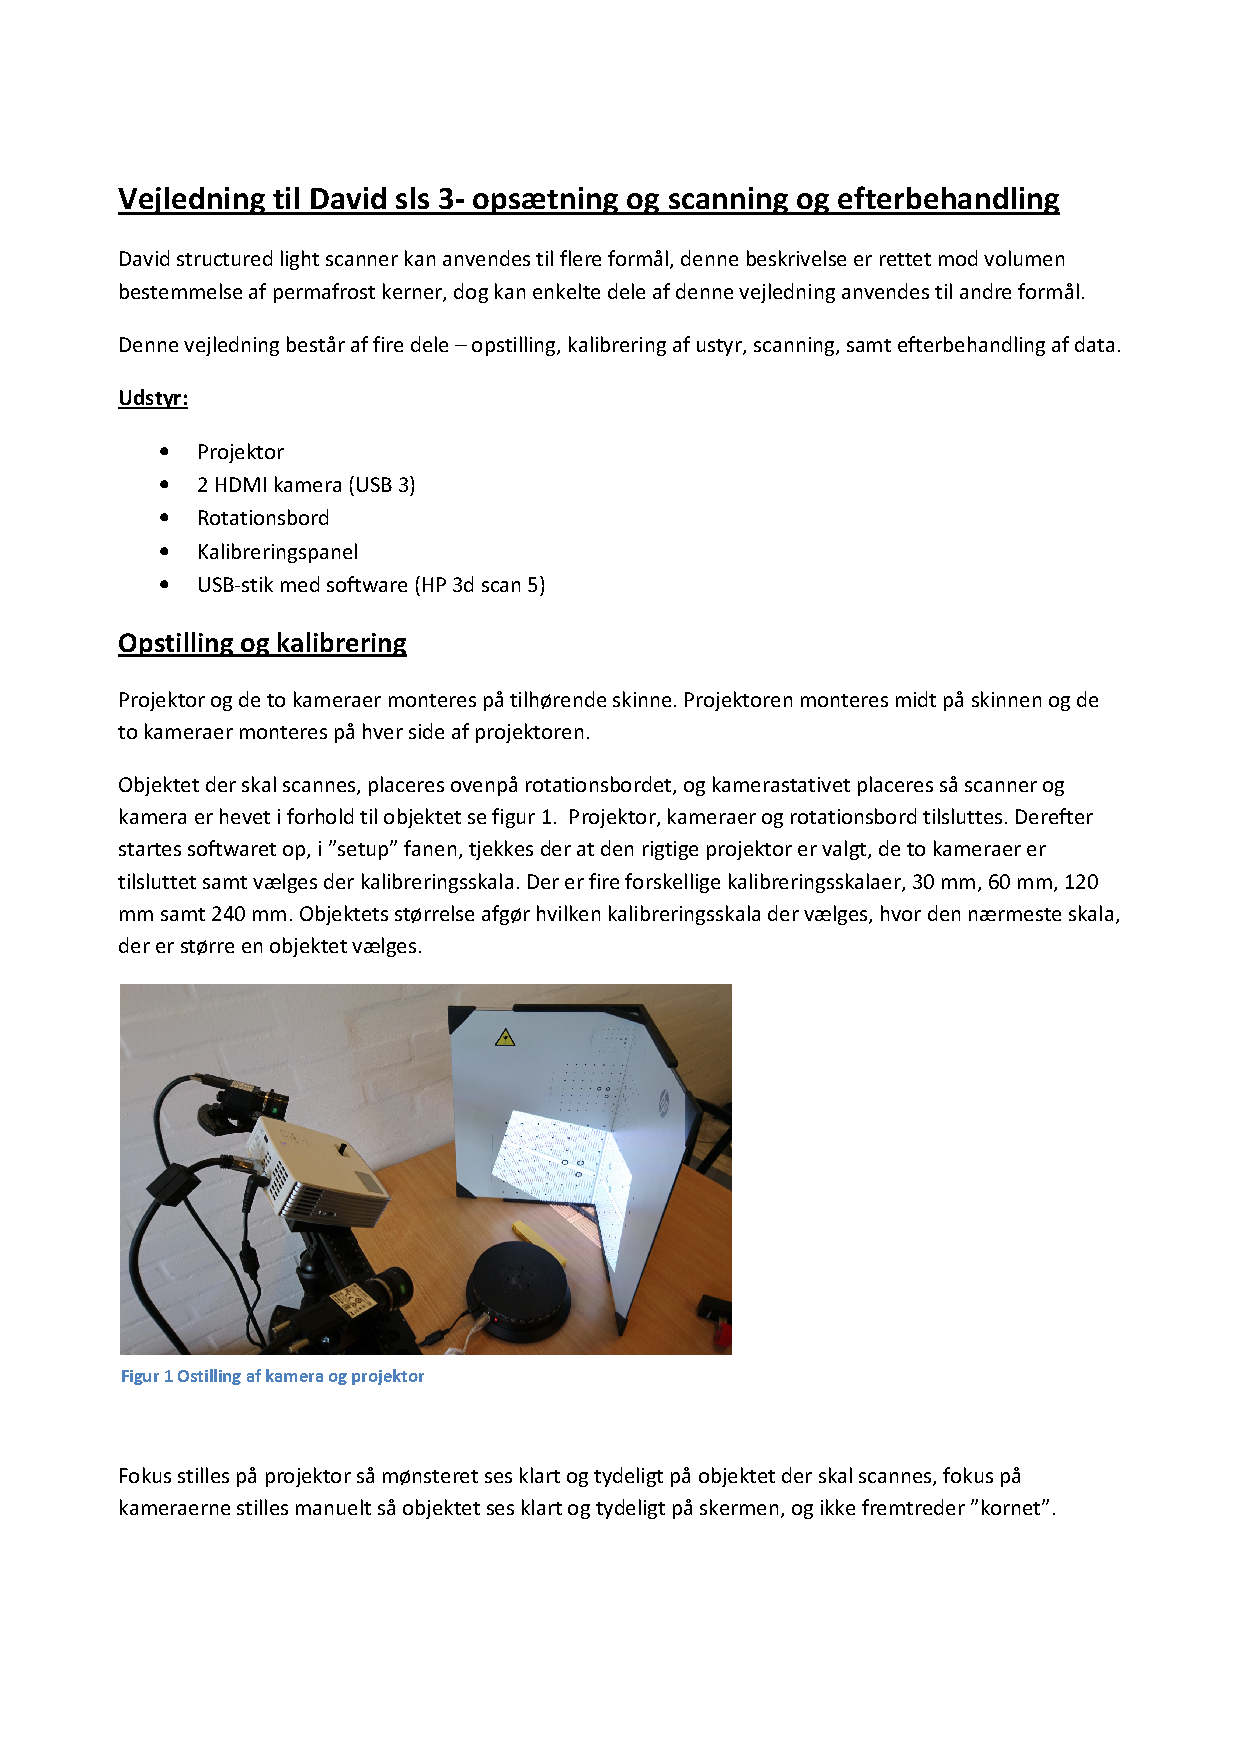
\includepdf[pages=-]{appendix/beskrivelse_scanning}




% -------------------------------------
% Bilag arkimedes-datablad isopar
% ---------------------------------
\clearpage
\FloatBlock
\chapter{Datablad Isopar-L}
\label{app:data_isopar}
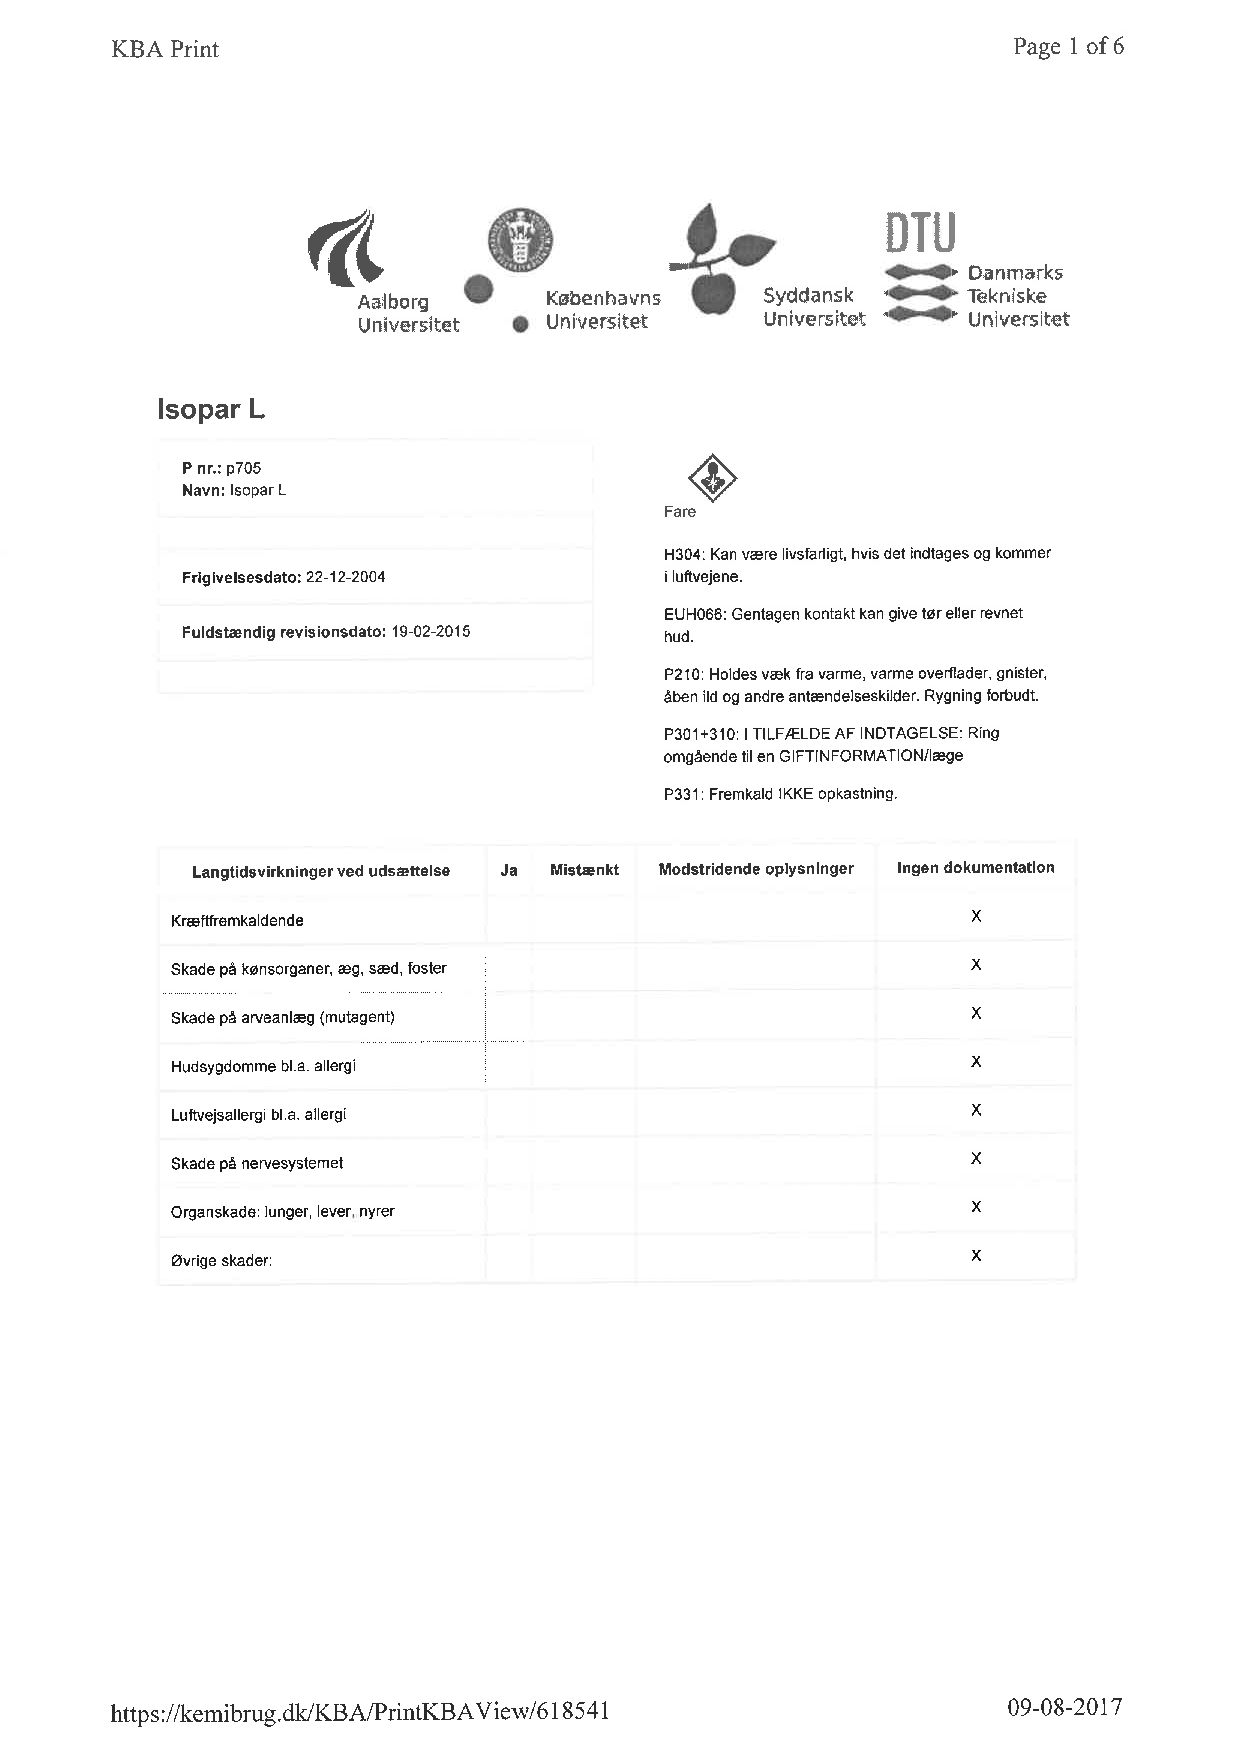
\includepdf[pages=-]{datablad_isopar.pdf}


% -------------------------------------
% Bilag målte dimmensioner terning
% ---------------------------------
\clearpage
\FloatBlock
\chapter{Målte dimmensioner af referenceobjekter}
\label{app:ref_obj_maalt}
\section{Terning}
Volumen er bestem ud fra gennemsnittet af bredde, lengde og højde målingerne i \vref{app:maalt_t} og bestemmes ved følgende formel:
\begin{equation}
V=l*b*h
\end{equation}
Volumen bestemmes til $124,22 \pm 0,08 cm^3$. 
Hvor standard afvigelsen findes ud fra formel:
\begin{equation}
\sigma_v=\sqrt[]{\sigma{b}^2+\sigma{l}^2+\sigma{h}^2}
\end{equation}
\begin{table}[h]
 \centering
% \caption{Terning, mål i $[mm]$, terningens dimensioner, bredden b, længden l og højden h}
  \topcaption{Mål i cm af terningens dimensioner, bredden $(b_1 -b_6)$, længden l $(h_1-h_6)$ og højden h $(h_1-h_6)$}
\label{app:maalt_t}  
\begin{tabular}{c c c c c c c c}
\toprule
b&4,99&	4,99&	4,99&	4,99&	4,98&	4,99&\\
l&	4,99&	4,99&	4,99&	5,00&	5,00&	5,00&\\
h&	5,00&	4,99&	4,99&	4,98&	4,98&	4,99&\\
\bottomrule
\end{tabular}
\end{table}

\section{Cylinder 2}
For at bestemme volumen af cylinder 2, deles cylinderen op i fem dele, hvor der bliver tre store dele og to mindre (to hvor udfresningerne er). Volumen af hvert enkelt element bestemmes ved et gennemsnit af r1, d1 osv. 
Følgende formel anvendes:
\begin{equation}
V_i=\pi*r_i^2*h_i
\end{equation}
Det totale volumen findes ved at summere fem elementer til $132,17 \pm 0,02 cm^3$, hvor standard afvigelsen findes ved formel:
\begin{equation}
\sigma_v=\sqrt[]{\sigma{d1}^2+\sigma{r1}^2+\sigma{d2}^2+\sigma{r2}^2...+\sigma{r5}^2}	
\end{equation}

\begin{table}
 \centering
% \caption{Terning, mål i $[mm]$, terningens dimensioner, bredden b, længden l og højden h}
% \label{app:maalt_t}
 \topcaption{Mål i cm af cylinderens dimensioner, radius $(r_1,r_2,r_3,r_4,r_5)$ og højden h $(h_1,h_2,h_3,h_4,h_5)$.}
\begin{tabular}{c c c }
\multicolumn{1}{l}{} & \multicolumn{1}{c}{$[cm]$} & \multicolumn{1}{c}{$[cm]$} \\ 
\toprule
$r_1$& 2,49 & 2,49 \\
$r_2$& 1,49 & 1,49 \\ 
$r_3$& 2,50 & 2,50 \\
$r_4$& 1,50 & 1,50\\
$r_5$& 2,50 & 2,50 \\
$h_1$& 1,98 & 1,98 \\
$h_2$& 0,99 & 0,98 \\
$h_3$& 2,00 & 2,01 \\
$h_4$& 0,98 & 0,95\\
$h_5$& 2,05 & 2,05\\
\bottomrule
\end{tabular}
\end{table}


% -------------------------------------
% Bilag refferance objekter scanning
% ---------------------------------
\clearpage
\FloatBlock
\chapter{Volumen af reference objekter, baseret på 3D scanning}
\label{app:3d_scan_vol}
Volumener $(Vol_1, Vol_2 og Vol_3)$ beregnet fra meshet punktsky ved brug af Python samt HP 3D scan software.  
Volumener markeret med $\dagger$ vurderes til ikke at være optimale, hvor der tydeligt kan ses en afvigelse i hvordan de separate elementer fra scanningen er sat sammen. Volumener opgivet i [$cm^3$]. 
 
 \begin{table}[h]
  \centering
  \topcaption{Referenceemner- terning og cylinder.}
  \label{tab:ref_vol_scan}
  \begin{tabular}{l c c c c| c c c c}
  \toprule
 \multicolumn{1}{l}{Referenceemne} & 	\multicolumn{1}{c}{Rotationsvinkel} & \multicolumn{3}{c}{Python [$cm^3$]} &	\multicolumn{3}{c}{HP [$cm^3$]}  \\
\midrule
 \multicolumn{1}{l}{} & 	\multicolumn{1}{c}{Grader[$^{\circ}$]} & \multicolumn{1}{c}{$Vol_1$} &  \multicolumn{1}{c}{$Vol_2$}  & \multicolumn{1}{c|}{$Vol_3$} &	\multicolumn{1}{c}{$Vol_1$}  & \multicolumn{1}{c}{$Vol_2$} & \multicolumn{1}{c}{$Vol_3$} \\
\cmidrule(r){1-1} \cmidrule(r){2-2} \cmidrule(r){3-3}
\cmidrule(r){4-4} \cmidrule(r){5-5} \cmidrule(r){6-6} \cmidrule(r){7-7} \cmidrule(l){8-8}

Terning & 45 & 122,01$\dagger$ & 123,56 & 124,02 & 121,37$\dagger$ & 123,78 & 124,55  \\
Cylinder 1 & 45 & 131,62 & 132,91 & 129,65$\dagger$ & 133,01 & 131,71 & 129,67$\dagger$ \\
  \bottomrule
  \end{tabular}
  \end{table}

% -------------------------------------
% Bilag arkimedes
% ---------------------------------
\clearpage
\FloatBlock
\chapter{Archimedes princip -- Forsøgs vejledning}
\label{app:arki_vejledning}
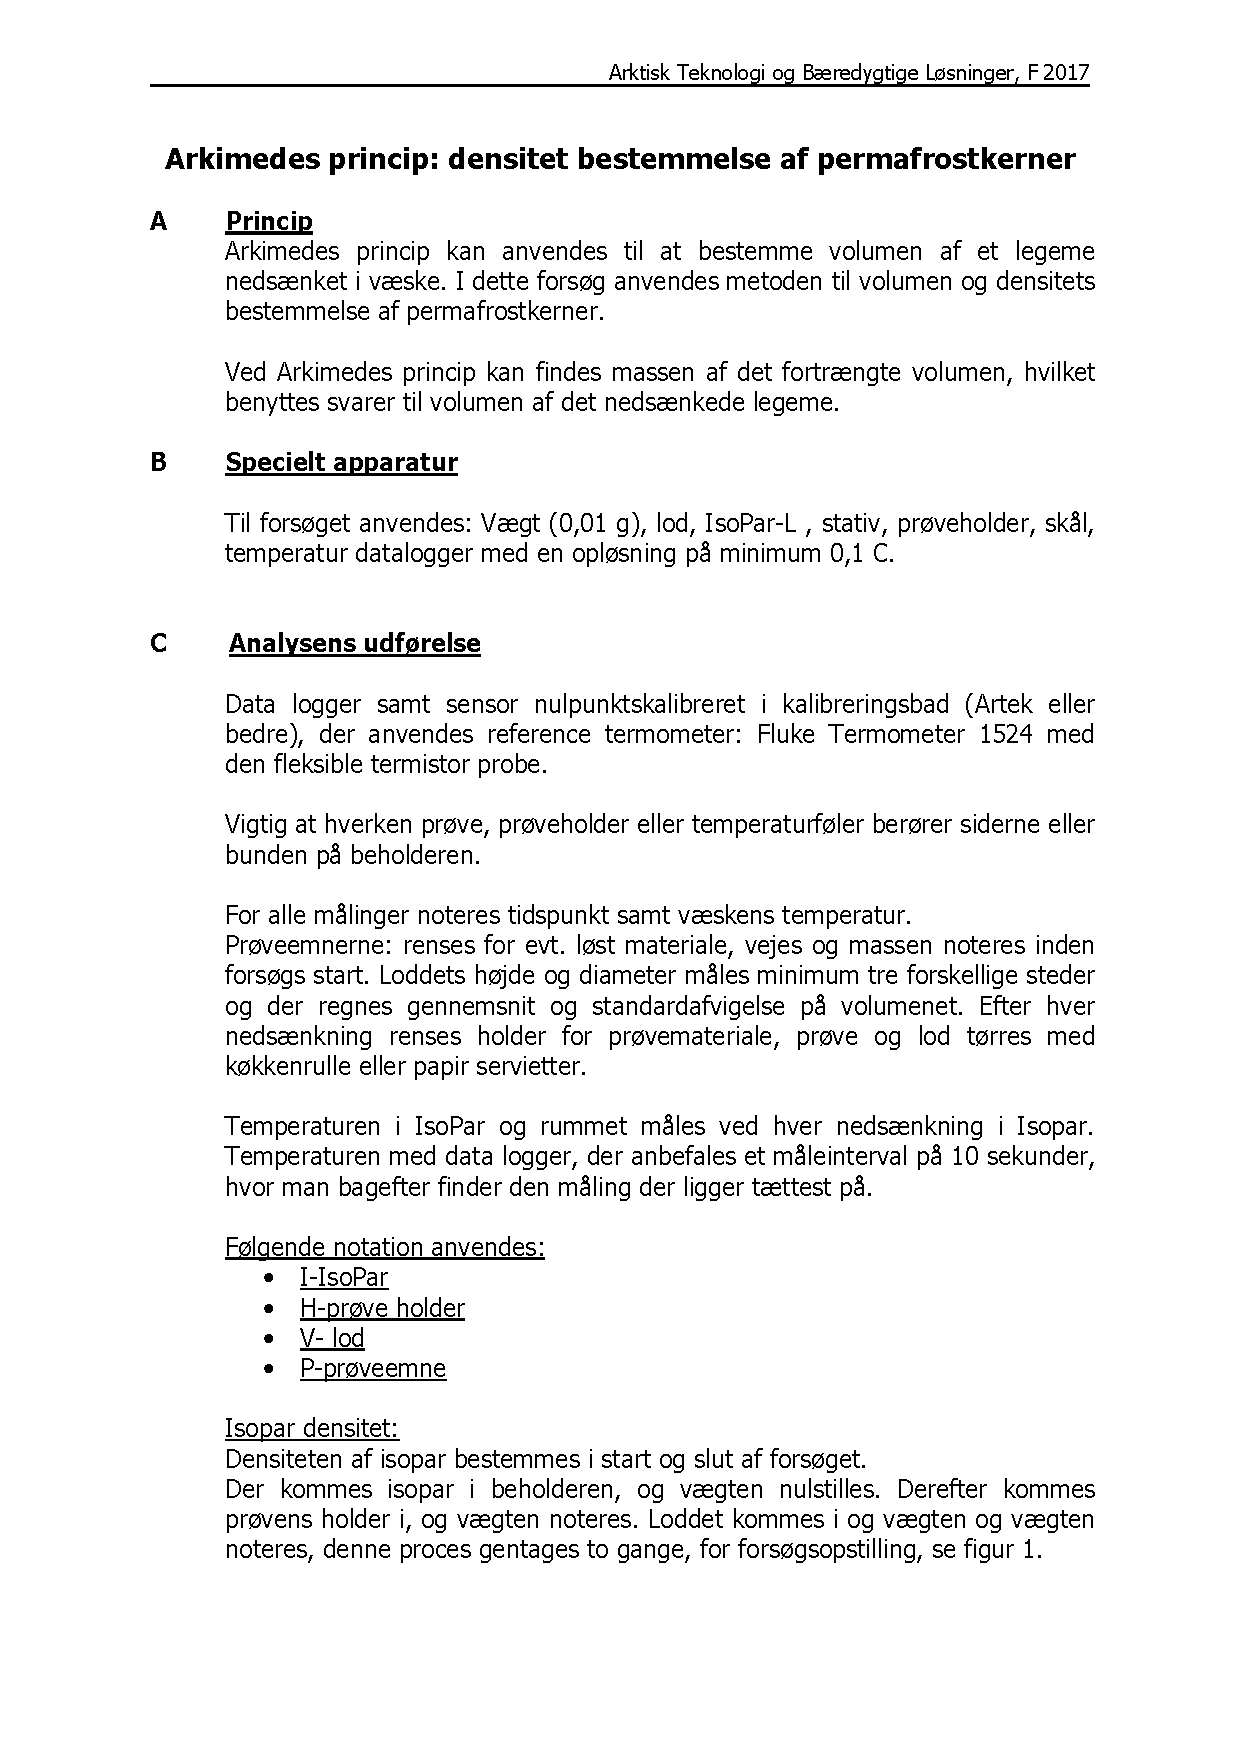
\includepdf[pages=-]{Arkimedes_princip.pdf}


% -------------------------------------
% Bilag skema arkimedes forsøg
% ---------------------------------
 \clearpage
 \FloatBlock
 \chapter{Forsøgs skema-- Archimedes princip}
 \label{app:skema_ark}
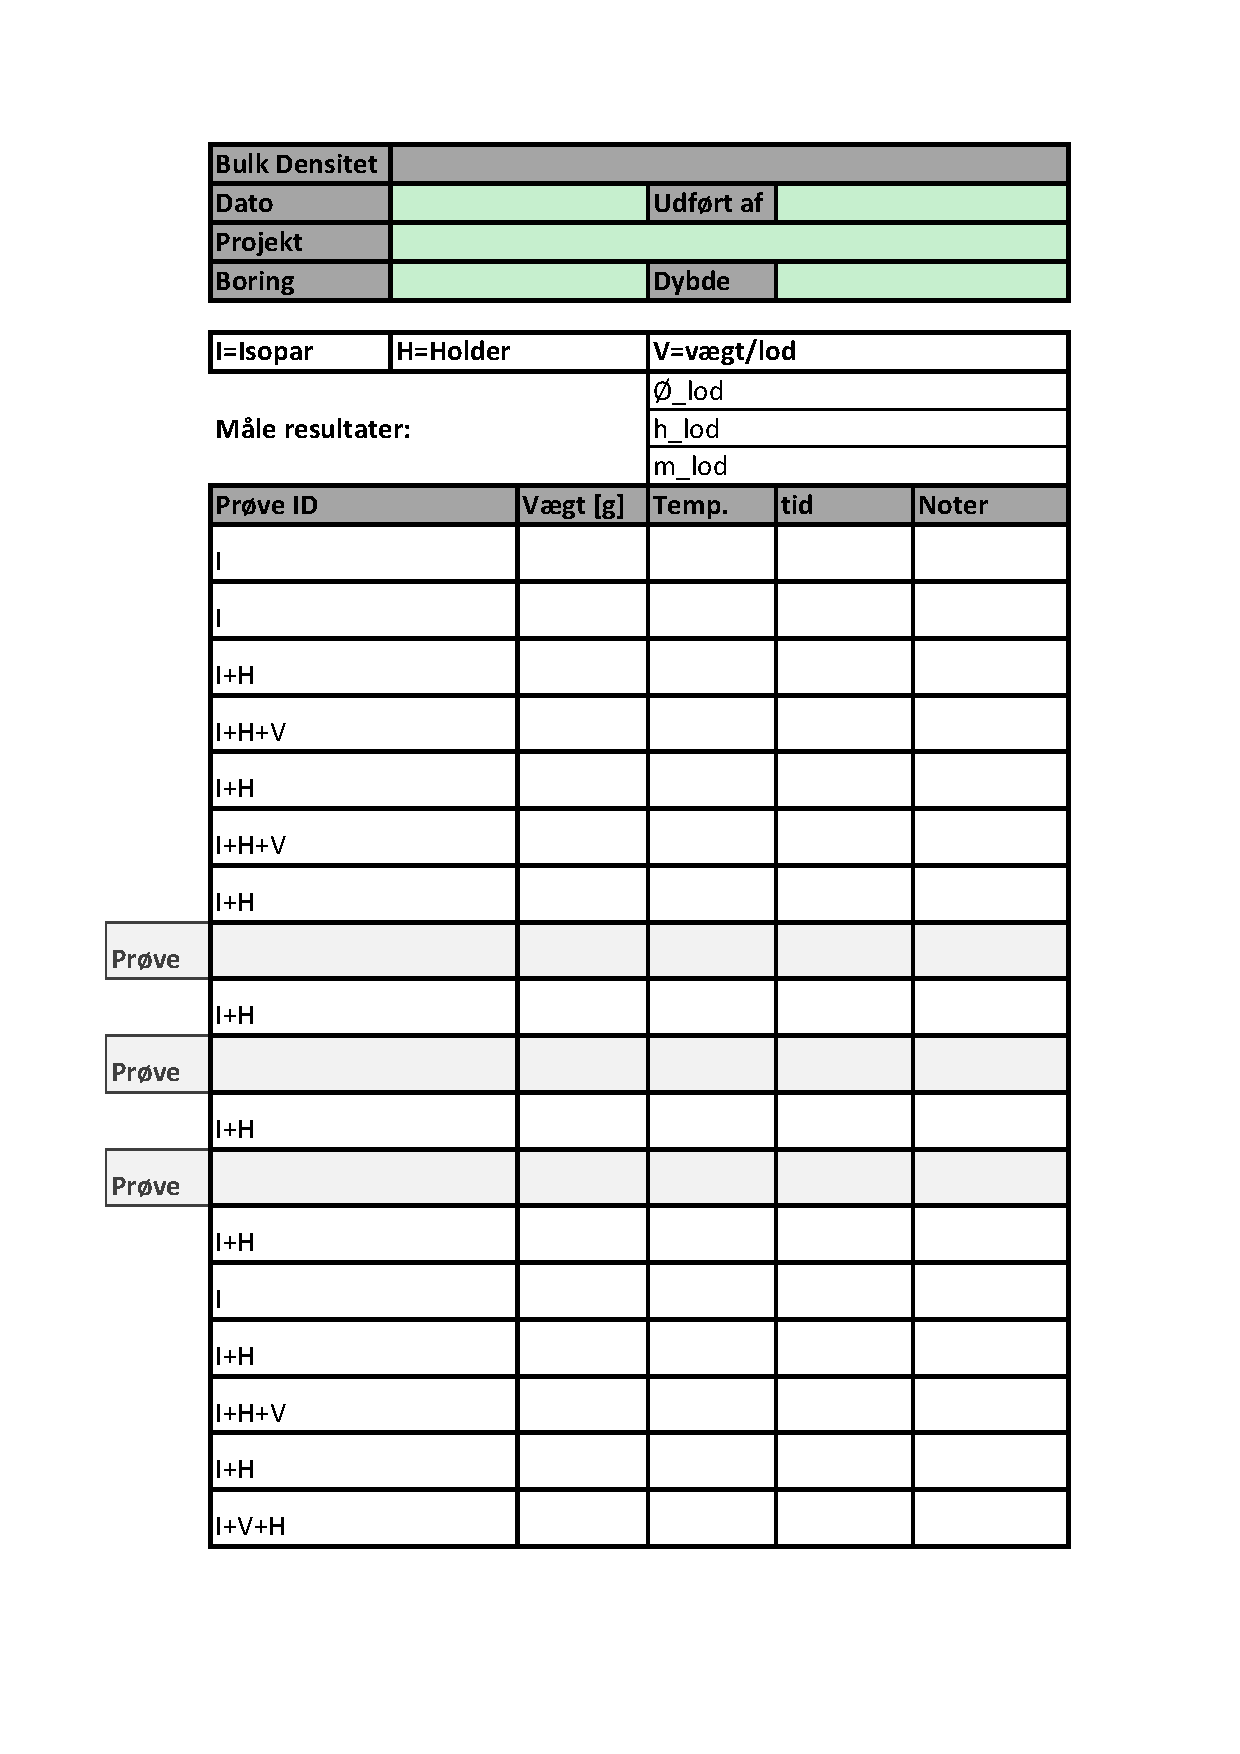
\includepdf[pages=-]{skema_arkimedes.pdf}

% % -------------------------------------
% % Rå data 3d scan
% % ---------------------------------
 \clearpage
 \FloatBlock
 \chapter{3D scanning -- Volumener og masse}
\label{app:scan}
\begin{landscape}
\begin{table}
\centering
\caption{3D scan, beregnede volumener ($Vol_1$, $Vol_2$ og $Vol_3$) ved brug af Python script og HP 3D scan software samt de prøvernes masse ($m_1$,$m_2$ og $m_3$) før scanning.}
\begin{tabular} {l c| D{.}{,}{3.2} D{.}{,}{3.2} D{.}{,}{3.2}| D{.}{,}{3.2} D{.}{,}{3.2} D{.}{,}{3.2}| D{.}{,}{3.2} D{.}{,}{3.2} D{.}{,}{3.2}}
\toprule
\multicolumn{1}{l}{Prøve} &\multicolumn{1}{c|}{Vinkel} & \multicolumn{3}{c|}{Python $[cm^3]$} & \multicolumn{3}{c|}{HP $[cm^3]$} & \multicolumn{3}{c}{Masse $[g]$}\\

\multicolumn{1}{l}{Boring\_lab. Nr.} & \multicolumn{1}{c|}{$[^{\circ}]$} & \multicolumn{1}{c}{$Vol_1$} & \multicolumn{1}{c} {$Vol_2$} & \multicolumn{1}{c|}{$Vol_3$} & \multicolumn{1}{c} {$Vol_1$} & \multicolumn{1}{c}{$Vol_2$} & \multicolumn{1}{c|} {$Vol_3$} & \multicolumn{1}{c}{$m_1$} & \multicolumn{1}{c}{$m_2$} & \multicolumn{1}{c}{$m_3$}\\

\cmidrule(r){1-1} \cmidrule(lr){2-2}	\cmidrule(r){3-5}	\cmidrule(r){6-8}	\cmidrule(r){9-11} 

$B16001\_6D$&45&396.61&401.12&401.71&396.56&401.02&401.72&458.45&458.69&458.50\\
$B16002\_5B$ & 45 &350.56&349.18&350.35&350.55&349.17&350.35&324.72&324.83&325.01\\
$B16003\_8D$ & 45 & 347.93 & 349.52 & 348.30 & 347.84 & 349.55 & 348.30 & 643.75 & 643.69 & 643.72\\
$B16004\_3F$ & 45 &368.26 & 366.12 & 368.80 & 368.23 & 366.10 & 368.78 & 517.96 & 518.30 & 517.95\\
$B16005T\_6E$ & 45 &195.02&195.77&199.93&195.01&195.76&199.93&220.83&220.79&220.57\\
$B16007\_7G$ & 45 &370.61&365.29&372.92&370.57&365.29&372.91&510.06&510.21&510.19\\
$B16009T\_7G$ & 45 &389.22&387.41&382.55&389.23&387.41&382.51&608.39&608.55&608.47\\
$B16010T\_7G$ & 45 &373.16&373.18&372.47&373.09&373.34&372.46&637.01&637.59&637.07\\
$B16011T\_7C$ & 45 &193.74 & 194.66 & 195.22 & 193.76 & 194.66 & 195.21 & 357.50 & 357.70 & 357.55\\
$B16012\_7D$ & 45 &393.18&389.50&393.09&393.18&389.69&393.04&708.83&710.18&709.31\\
$B16013T\_5C$ & 45 &391.11&392.29&392.59&391.11&392.16&392.59&624.97&625.05&625.17\\
$B16014\_4F$ & 45 &386.90&386.03&385.45&386.86&385.78&385.41&574.92&574.74&575.07\\
$B16015T\_5D$ & 45 &416.77&416.48&415.79&416.76&416.45&415.75&753.94&753.99&754.07\\
$B16019T\_8F$ & 45 &377.65&375.77&376.50&377.68&375.79&376.45&722.36&722.48&722.37\\
$B16022T\_4C$ & 45 &196.88&197.40&197.21&196.87&197.39&197.21&327.83&324.27&324.18\\
\cmidrule(lr){1-11}
$B16002\_5B$ & 60 &353.87&356.89&357.47&353.84&356.88&357.47&324.45&324.80&324.32\\
$B16004\_3F$ & 60 &369.28&366.92&367.99&369.23&366.88&367.98&517.67&517.60&517.64\\
$B16012\_7D$ & 60 &390.41&391.98&397.85&390.41&391.96&397.80&708.65&708.43&708.14\\
$B16019T\_8F$ & 60 &378.73&371.26&374.17&378.68&372.97&374.16&722.39&722.50&722.45\\
\cmidrule(lr){1-11}
$B16002\_5B$ & 72 &351.44&357.77&355.83&351.44&357.71&355.76&324.20&324.16&324.12\\
$B16004\_3F$ & 72 &367.91&367.23&368.50&367.86&367.20&368.45&517.55&517.51&517.49\\
$B16012\_7D$ & 72 &391.90&388.84&392.06&391.90&388.78&392.05&707.98&707.61&707.47\\
$B16019T\_8F$ & 72 &378.09&376.01&375.91&378.07&376.02&375.89&722.34&722.37&722.37\\
\bottomrule
\end{tabular}
\end{table}
\end{landscape}


% -------------------------------------
% Gennemsnit vol scanning
% ---------------------------------
\clearpage
 \FloatBlock
 \chapter{3D scanning -- Beregnede densiteter}
 \label{app:vol_snitt}
\begin{landscape}
\begin{table}[h]
 \centering
 \topcaption{Prøve - lab Nr., rotationsvinkel og densitet $[g/cm^3]$, beregnet for hver enkel scanning ($\rho_1,\rho_2 og \rho_3$) med hhv. python script og hp 3D scan software, middelværdien for bulkdensiteten er opgivet med $\pm$ en spredning.}
  \begin{tabular}{l c| D{.}{,}{2.2} D{.}{,}{2.2} D{.}{,}{2.2}| D{.}{,}{2.2} D{.}{,}{2.2} D{.}{,}{2.2}| D{.}{\pm}{4.4} D{.}{\pm}{4.4}}
 \toprule
 \multicolumn{1}{l}{Prøve} & \multicolumn{1}{c|}{Vinkel} & \multicolumn{3}{c|}{Python} &	\multicolumn{3}{c|}{HP} & \multicolumn{1}{c}{Avg. Python} &\multicolumn{1}{c}{Avg. HP} \\

 \multicolumn{1}{l}{Boring\_lab.} & \multicolumn{1}{c|}{$[^{\circ}]$} & \multicolumn{3}{c|}{$[g/cm^3]$} & \multicolumn{3}{c|}{$[g/cm^3]$} & \multicolumn{1}{c}{$[g/cm^3]$} & \multicolumn{1}{c}{$[g/cm^3]$}\\
\cmidrule(r){1-1} \cmidrule(r){2-2} \cmidrule(r){3-5} \cmidrule(r){6-8} \cmidrule(r){9-10}
  $B16001\_6D$&45&1.16&1.14&1.14&1.16&1.14&1.14&1,15 . 0,01&1,15 . 0,01\\
$B16002\_5B$&45&0.93&0.93&0.93&0.93&0.93&0.93&0,93 . 0,00 & 0,93 . 0,00\\
$B16003\_8D$&45&1.85&1.84&1.85&1.85&1.84&1.85&1,85 . 0,00&1,85 . 0,00\\
$B16004\_3F$&45&1.41&1.42&1.40&1.41&1.41&1.40&1,41 . 0,01&1,41 . 0,01\\
$B16005T\_6E$&45&1.13&1.13&1.10&1.13&1.13&1.10&1,12 . 0,02&1,12 . 0,01\\
$B16007\_7G$&45&1.38&1.40&1.37&1.38&1.40&1.37&1,38 . 0,01&1,38 . 0,01\\
$B16009T\_7G$&45&1.56&1.57&1.59&1.56&1.57&1.59&1,57 . 0,01&1,57 . 0,01\\
$B16010T\_7G$&45&1.71&1.71&1.71&1.71&1.71&1.71&1,71 . 0,00&1,71 . 0,00\\
$B16011T\_7C$&45&1.85&1.84&1.83&1.85&1.84&1.83&1,84 . 0,01&1,84 . 0,01\\
$B16012\_7D$&45&1.80&1.82&1.80&1.80&1.82&1.80&1,81 . 0,01&1,81 . 0,01\\
$B16013T\_5C$&45&1.60&1.59&1.59&1.60&1.59&1.59&1,59 . 0,00 &1,59 . 0,00\\
$B16014\_4F$&45&1.49&1.49&1.49&1.49&1.49&1.49&1,49 . 0,00&1,49 . 0,00\\
$B16015T\_5D$&45&1.81&1.81&1.81&1.81&1.81&1.81&1,81 . 0,00&1,81 . 0,00\\
$B16019T\_8F$&45&1.91&1.92&1.92&1.91&1.92&1.92&1,92 . 0,00 &1,92 . 0,00\\
$B16022T\_4C$&45&1.67&1.64&1.64&1.67&1.66&1.66&1,65 . 0,01&1,66 . 0,00\\
\cmidrule (lr){1-10}
$B16002\_5B$&60&0.92&0.91&0.91&0.92&0.91&0.91&0,91 . 0,00&0,91 . 0,00 \\
$B16004\_3F$&60&1.40&1.41&1.41&1.40&1.41&1.41&1,41 . 0,00 &1,41 . 0,00\\
$B16012\_7D$&60&1.82&1.81&1.78&1.82&1.81&1.78& 1,80 . 0,02 &1,80 . 0,02\\
$B16019T\_8F$&60&1.91&1.95&1.93&1.91&1.94&1.93&1,93 . 0,02&1,93 . 0,02\\
\cmidrule (lr){1-10}
$B16002\_5B$&72&0.92&0.91&0.91&0.92&0.91&0.91&0,91 . 0,01&0,91 . 0,01\\
$B16004\_3F$&72&1.41&1.41&1.4&1.41&1.41&1.4&1,41 . 0,00&1,41 . 0,00\\
$B16012\_7D$&72&1.81&1.82&1.8&1.81&1.82&1.81&1,81 . 0,01&1,81 . 0,01\\
$B16019T\_8F$&72&1.91&1.92&1.92&1.91&1.92&1.92&1,92 . 0,01&1,92 . 0,01\\
 \bottomrule
 \end{tabular}
 \end{table}
\end{landscape}

% -------------------------------------
% Deklination
% ---------------------------------
\clearpage
 \FloatBlock
 \chapter{3D scan --Gennemsnitlig bulkdensitet}
 \label{app:dens_sdtot}
\begin{table}
 \centering
 \topcaption{Gennemsnitlig bulkdensitet for prøver scannet med 3D scanner. Prøve\-lab Nr., rotationsvinkel og densitet angivet i [$g/cm^3$] $\pm$ en spredning.}
  \begin{tabular}{l c D{.}{\pm}{5.5} D{.}{\pm}{5.5}}
 \toprule
 \multicolumn{1}{l}{Prøve} & \multicolumn{1}{c}{Vinkel} & \multicolumn{1}{c}{Python} &	\multicolumn{1}{c}{HP} \\

 \multicolumn{1}{c}{Boring\_lab. Nr.} & \multicolumn{1}{c}{$[^{\circ}]$} & \multicolumn{1}{c}{$[g/cm^3]$} & \multicolumn{1}{c}{$[g/cm^3]$}\\
\cmidrule(r){1-1} \cmidrule(r){2-2} \cmidrule(r){3-3} \cmidrule(r){4-4}
  $B16001\_6D$ & 45 & 1,15 . 0,01 & 1,15 . 0,01 \\
$B16002\_5B$ & 45 & 0,93 . 0,00 & 0,93 . 0,00\\
$B16003\_8D$ & 45 & 1,85 . 0,00 & 1,85 . 0,00\\
$B16004\_3F$ & 45 & 1,41 . 0,01 & 1,41 . 0,01\\
$B16005T\_6E$ & 45 & 1,12 . 0,02 & 1,12 . 0,02\\
$B16007\_7G$ & 45 & 1,38 . 0,01 & 1,38 . 0,01\\
$B16009T\_7G$ & 45 & 1,57 . 0,01 & 1,58 . 0,01\\
$B16010T\_7G$ & 45 & 1,71 . 0,00& 1,71 . 0,00\\
$B16011T\_7C$ & 45 & 1,84 . 0,01 & 1,84 . 0,01\\
$B16012\_7D$ & 45 & 1,81 . 0,01 & 1,81 . 0,01\\
$B16013T\_5C$ & 45 & 1,59 . 0,00 & 1,59 . 0,00\\
$B16014\_4F$ & 45 & 1,49 . 0,00 & 1,49 .0,00 \\
$B16015T\_5D$ & 45 & 1,81 . 0,00 & 1,81 . 0,00\\
$B16019T\_8F$ & 45 & 1,92 . 0,00 & 1,92 . 0,00\\
$B16022T\_4C$ & 45 & 1,65 . 0,01 & 1,65 . 0,01\\
\cmidrule (lr){1-4}
$B16002\_5B$ & 60 & 0,91 . 0,01 & 0,91 . 0,01\\
$B16004\_3F$ & 60 & 1,41 . 0,00 & 1,41 . 0,00\\
$B16012\_7D$ & 60 & 1,80 . 0,02 & 1,80 . 0,02\\
$B16019T\_8F$ & 60 & 1,93 . 0,02 & 1,93 . 0,02\\
\cmidrule (lr){1-4}
$B16002\_5B$ & 72 & 0,91 . 0,01 & 0,91 . 0,01\\
$B16004\_3F$ & 72 & 1,41 . 0,00 & 1,41 . 0,00\\
$B16012\_7D$ & 72 & 1,81 . 0,01 & 1,81 . 0,01\\
$B16019T\_8F$ & 72 & 1,92 . 0,01 & 1,92 . 0,01\\
 \bottomrule
 \end{tabular}
 \end{table}

% -------------------------------------
% Arkimedes pb
% ---------------------------------
 \clearpage
 \FloatBlock
 \chapter{Arkimedes -- Kalibrering af temperatur sensorer}
 \label{fig:temp_plot} 
Kalibrering af temperatursensor har foregået den 17 juli- 2017, målingerne strækekr sig over 1 time og 17 minutter. De udslag der er ses på plottet i på næste side er indenfor dataloggerens måleopløsning. Gennemsnittet af målingerne på hhv. "channel 1" og "channel 2" trukket fra temperaturmålingerne udført ved bestemmelse af bulkdensitet.
\begin{landscape}
\begin{figure}
\centering
\caption{Kalibrering af tenmperatur sensor plot, temperatur som funktion af tiden}
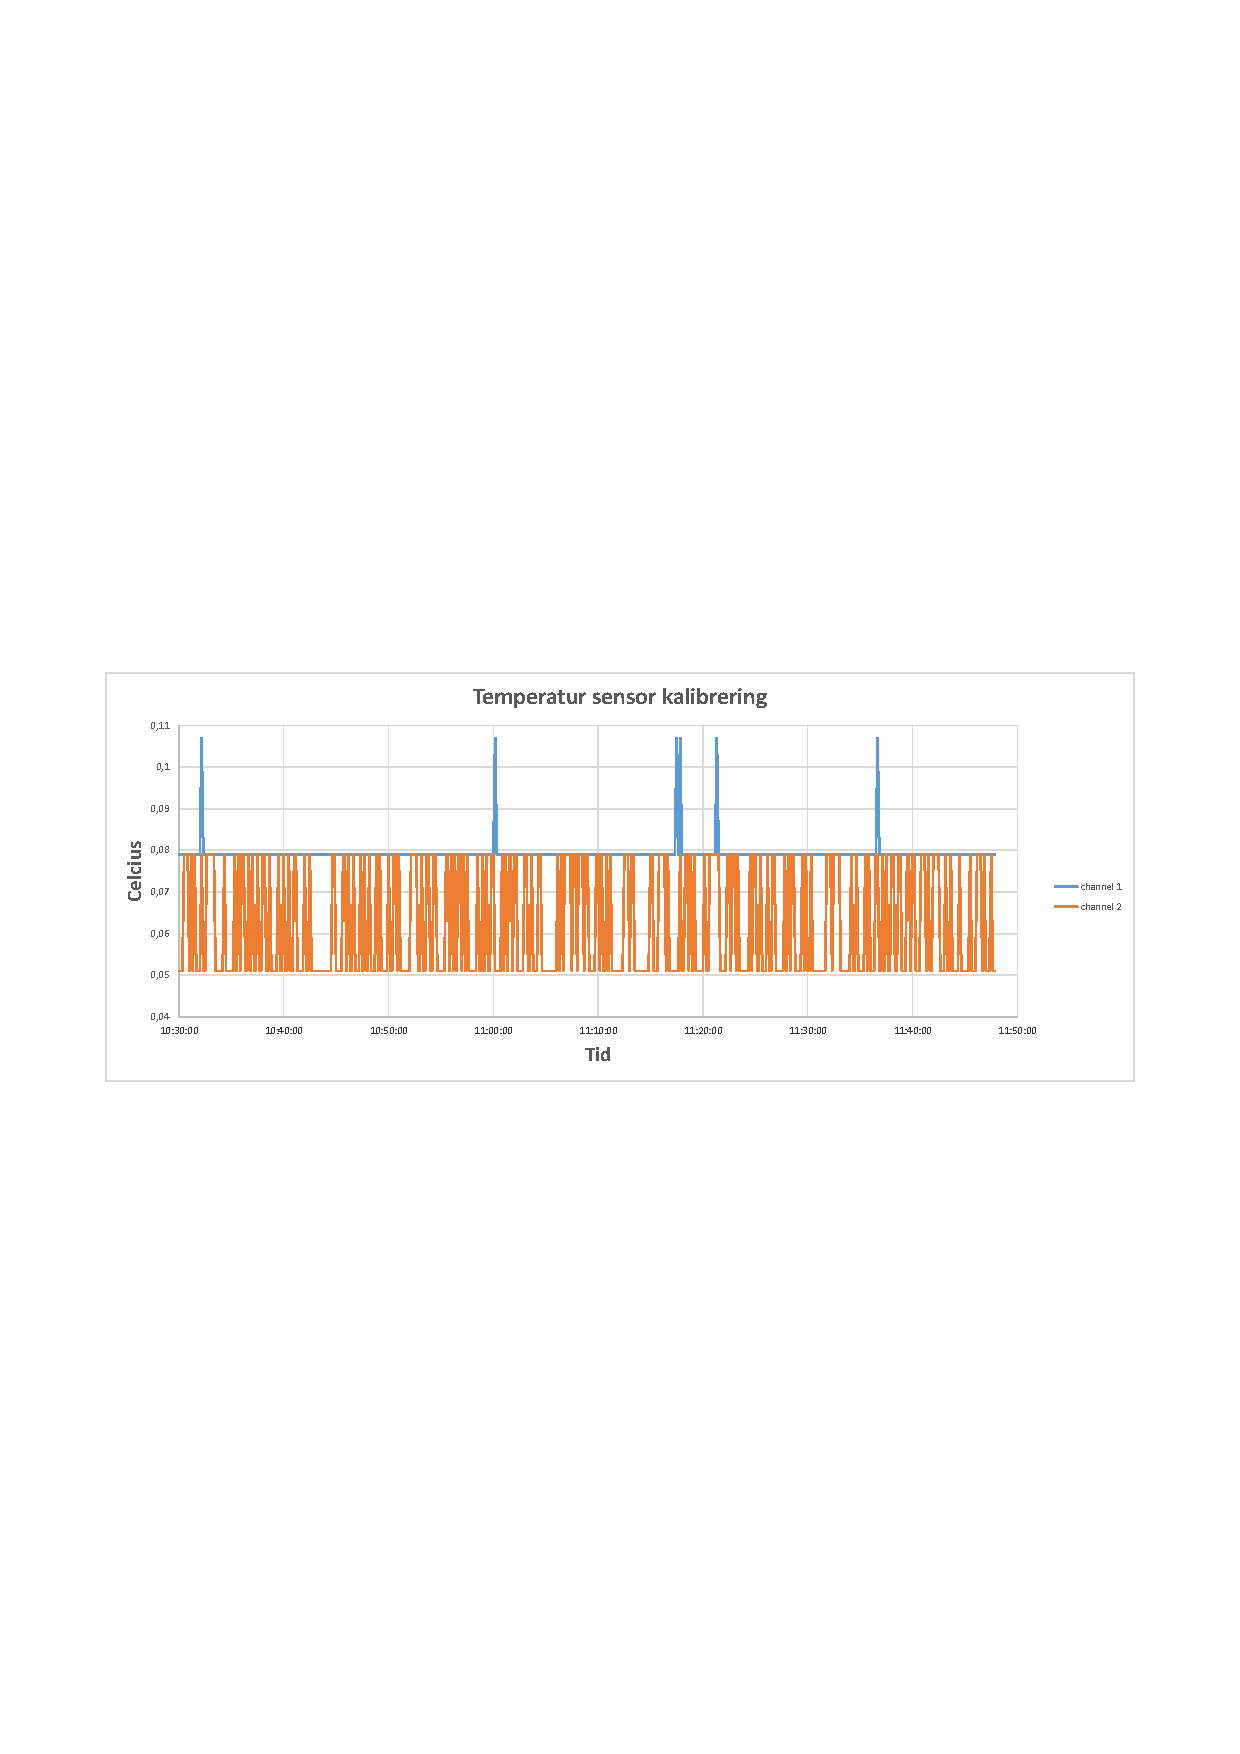
\includegraphics[width=1.2\textwidth]{appendix/t_sens_kal_plot}
% \caption{Kalibrering af tenmperatur sensor plot, temperatur som funktion af tiden}
\end{figure}
\end{landscape}


% -------------------------------------
% Arkimedes pb
% ---------------------------------
 \clearpage
 \FloatBlock
 \chapter{Arkimedes -- Bulk densitet}
 \label{app:arki_pb_res}
\begin{table}[h]
 \centering
 \topcaption{Bulk densitet $\rho_b$ beregnet på bagrund af volutmetrisk bestemmelse ved Archimedes princip. Prøve - lab Nr. og bulk densitet $g/cm^3$ $\pm$ standardafvigelse. Prøver markeret med $\dagger$ angiver luftbobler der kommer ud af kerner under neddykning og prøve markeret med $\ddagger$ angiver at der blev observeret en større mængde luftbobler. Luftboblerne giver variation i volumen bestemmelserne for den enkelte kerne, dog er variationen så lille at den ikke harver væsentlig betydning for den beregnede bulkdensitet.}
  \begin{tabular}{l D{.}{\pm}{5.5} l}
 \toprule
 \multicolumn{1}{l}{Prøve} & \multicolumn{1}{c}{$\rho_b$} \\

 \multicolumn{1}{c}{Boring\_lab. Nr.} & \multicolumn{1}{c}{$[g/cm^3]$} \\
\cmidrule(r){1-1} \cmidrule(r){2-2} \cmidrule(r){3-3} 
  $B16001T\_6D$&	1,16.	0,01\\
$B16002\_5B$&	0,98.	0,03 \ddagger\\
$B16003\_8D$&	1,87.	0,00\\
$B16004\_3F$&	1,43.	0,01\dagger \\
$B16005T\_6E$&	1,12.	0,00\\
$B16007\_7G$&	1,39.	0,00\\
$B16009T\_7G$&	1,60.	0,01\\
$B16010T\_7G$&	1,74.	0,01\\
$B16011T\_7C$&	1,87.	0,00\\
$B16012\_7D$&	1,85.	0,01\\
$B16013T\_5C$&	1,61.	0,01\\
$B16014\_4F$&	1,51.	0,01\\
$B16015T\_5D$&	1,83.	0,01\dagger\\
$B16019T\_8F$&	1,93.	0,00\dagger \\
$B16022T\_4C$&	1,67.	0,00\\

 \bottomrule
 \end{tabular}
 \end{table}


% -------------------------------------
% Arkimedes pb
% ---------------------------------
%  \clearpage
 \FloatBlock
 \chapter{Arkimedes -- Isopar densitet som funktion af temperaturen}
 \label{fig:iso_dens_plot}
Densitet af isopar som funktionen af temperaturen, punkterne plottet er et gennemsnit af de to beregnede densiteter for hvert prøvemne. Hvor de angivne usikkerheder i x og y-retning er et udtryk for variationen i de to målinger, temperatur og $\rho_iso$ for hvert prøvemne. 
\begin{landscape}
\begin{figure}[h]
\centering
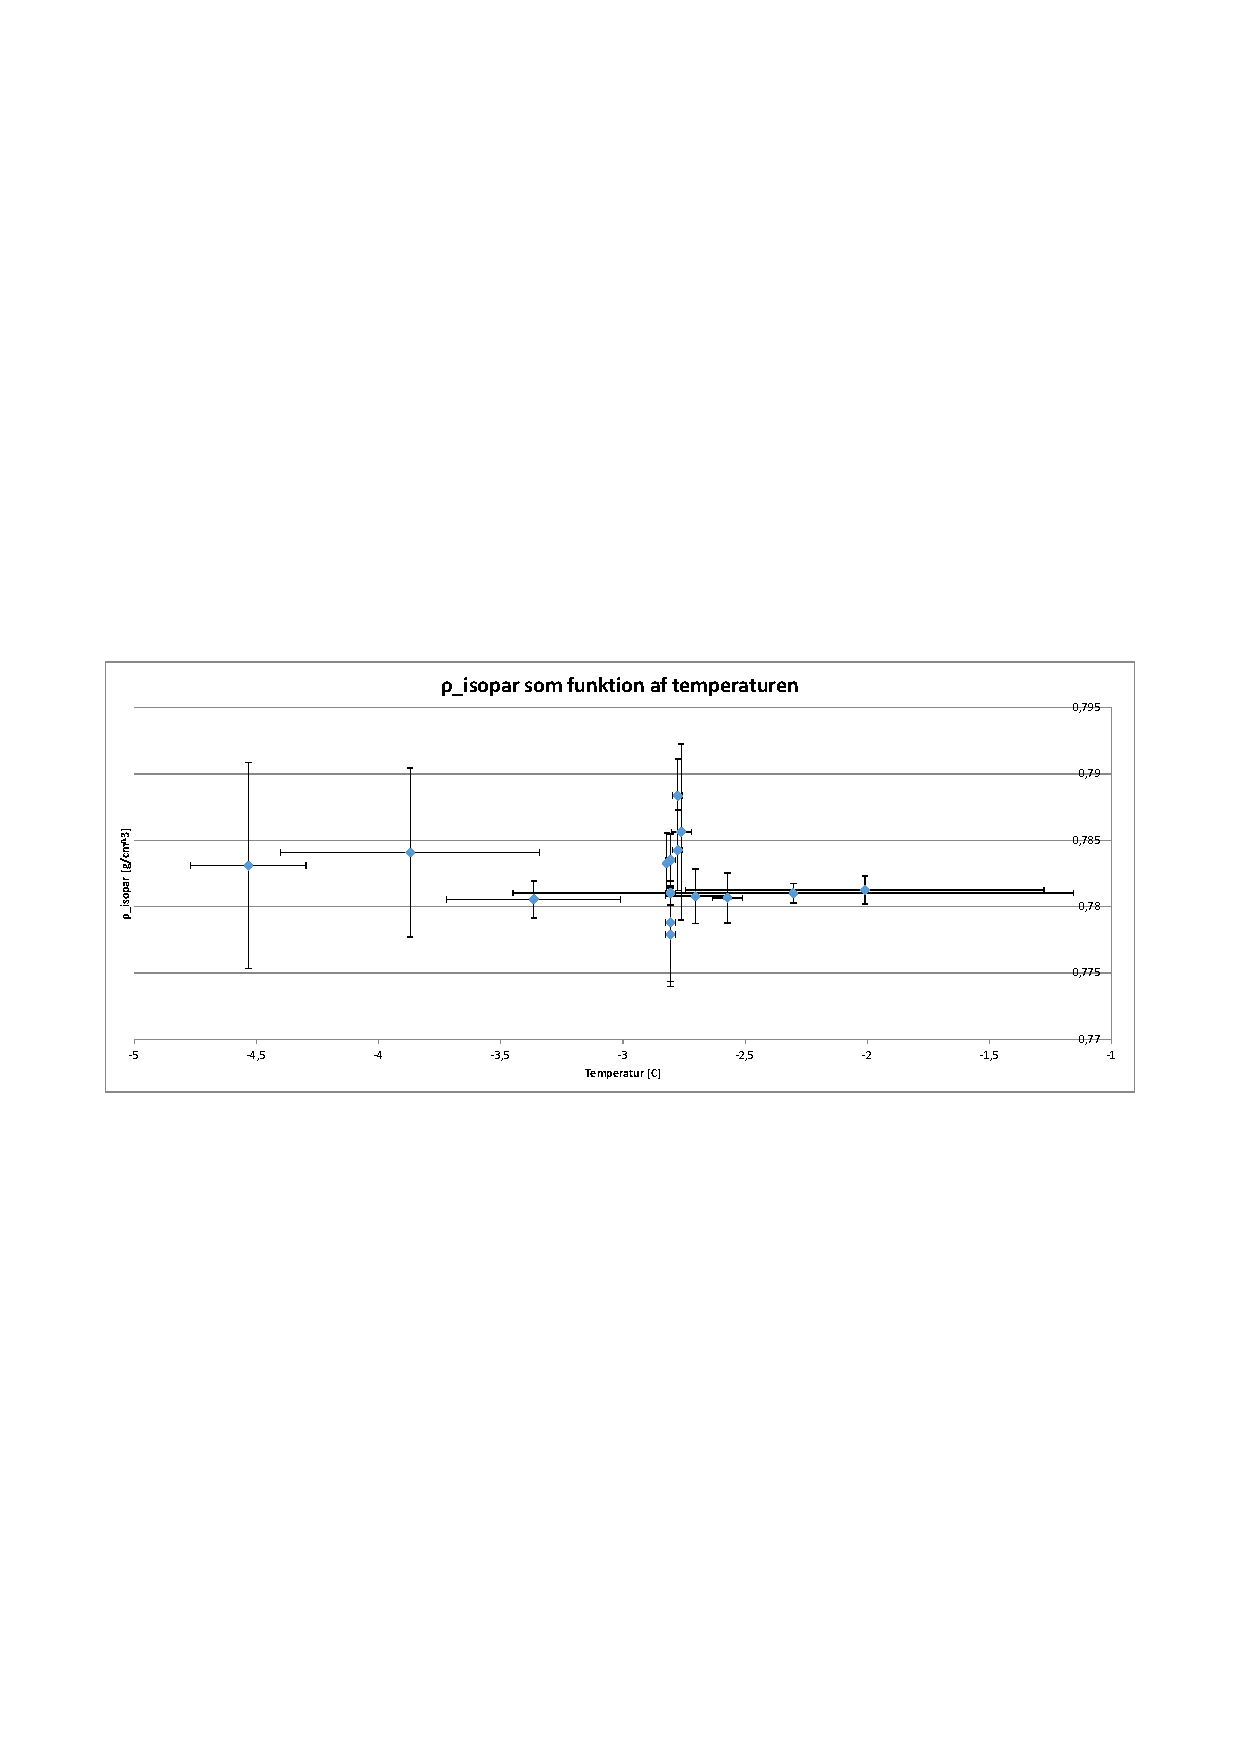
\includegraphics[width=1.2\textwidth]{appendix/ny_tab_dens_plot}
\caption{Isopars gennemsnitsdensitet for hvert enkelt prøveemne plottet som funktion af temperaturen.}
\end{figure}
\end{landscape}



% -------------------------------------
% Arkimedes rå
% ---------------------------------
 \clearpage
 \FloatBlock
 \chapter{Arkimedes -- Rå-data}
 \label{app:scan}
\centering
\begin{longtable}{l c c c c}
\caption{Rå-data, bulk densitet bestemmelse ved Archimedes princip}
\\
\toprule
\multicolumn{1}{l}{Prøve} & \multicolumn{1}{c}{Masse} & \multicolumn{1}{c}{Tid}
& \multicolumn{1}{c}{Temperatur} & \multicolumn{1}{c}{Kommentar} 
\\
\multicolumn{1}{c}{} & \multicolumn{1}{c}{opstilling} & \multicolumn{1}{c}{} & \multicolumn{1}{c}{isopar} & \multicolumn{1}{c}{} 
\\

\multicolumn{1}{c}{} & \multicolumn{1}{c}{$[g]$} &\multicolumn{1}{c}{$[tt:mm:ss]$} & \multicolumn{1}{c}{$[\celsius]$} & \multicolumn{1}{c}{} 
\\

 \cmidrule(r){1-1} \cmidrule(r){2-2}	\cmidrule(r){3-3}	\cmidrule(r){4-4} \cmidrule(r){5-5}	

\endfirsthead

\caption[]{rå-data, bulk densitet bestemmelse ved arkimedes princip (fortsat)}
\\
\toprule
\multicolumn{1}{l}{Prøve} & \multicolumn{1}{c}{Masse} & \multicolumn{1}{c}{Tid}
& \multicolumn{1}{c}{Temperatur} & \multicolumn{1}{c}{Kommentar} 
\\

\multicolumn{1}{c}{} & \multicolumn{1}{c}{opstilling} & \multicolumn{1}{c}{} & \multicolumn{1}{c}{isopar} & \multicolumn{1}{c}{} 
\\

\multicolumn{1}{c}{} & \multicolumn{1}{c}{$[g]$} &\multicolumn{1}{c}{$[tt:mm:ss]$} & \multicolumn{1}{c}{$[\celsius]$} & \multicolumn{1}{c}{} 
\\

 \cmidrule(r){1-1} \cmidrule(r){2-2}	\cmidrule(r){3-3}	\cmidrule(r){4-4} \cmidrule(r){5-5}	

\endhead
\bottomrule
\multicolumn{5}{r}{\textit{tabellen fortsættes}}
\endfoot

\bottomrule
\endlastfoot
 I	&2869,74	&10:38:40&	-\\
I	&0,00		&10:38:40&	-\\
I+H	&5,16		&10:39:30&	-4,28\\
I+H+L	&72,38		&10:40:20&	-4,76\\
I+H	&3,84		&10:40:50&	-4,73\\
I+H+L	&71,01		&10:41:20&	-4,70\\
I+H	&2,78		&10:42:00&	-4,70\\
I+H	&2,82		&10:42:20&	-4,70\\
$B16001T\_6D$	&309,50	&10:43:00&	-4,70\\
I+H	&-4,93		&10:44:30&	-4,58\\
$B16001T\_6D$	&301,12	&10:45:10&	-4,58\\
I+H	&-8,36		&10:46:10&	-4,55\\
$B16001T\_6D$	&300,10	&10:47:00&	-4,52\\
\hline
I+H	&-12,70		&10:47:50&	-4,55\\
I	&-17,76		&10:51:50&	-\\
I+H	&-13,15		&10:52:30&	-3,89\\
I+V+H	&54,97		&10:53:20&	-4,37\\
I+H	&-13,27		&11:02:30&	-4,04\\
$B16009T\_7G$	&279,20	&11:03:20&	-4,13\\
I+H	&-22,42		&11:04:20&	-4,04\\
$B16009T\_7G$	&274,40	&11:05:10&	-4,01\\
I+H	&-28,42		&11:05:50&	-4,01\\
$B16009T\_7G$	&268,90	&11:06:30&	-4,01\\
\hline
I+H	&-30,12		&11:07:30&	-3,56\\
I	&-36,67		&11:08:00&	-\\
I+H	&-33,24		&11:08:40&	-3,29\\
I+V+H	&34,10		&11:09:00&	-3,62\\
I+H	&-34,72		&11:15:30&	-3,20\\
\newpage
$B16015T\_5D$	&278,15	&11:16:10&	-3,23 & Luftbobler\\
I+H	&-45,06		&11:17:30&	-3,26\\
$B16015T\_5D$	&275,66	&11:18:10&	-3,29\\
I+H	&-48,66		&11:18:50&	-3,23\\
$B16015T\_5D$	&272,14	&11:19:10&	-3,23\\
\hline
I+H	&-51,55		&11:20:00&	-3,17\\
I	&-58,31		&11:21:00&	-\\
I+H	&-51,49		&11:21:30&	-2,79\\
I+H+L	&16,02		&11:22:00&	-3,11\\
I+H	&-55,52		&11:29:20&	-2,85\\
$B16007\_7G$	&230,68	&11:30:00&	-2,76\\
I+H	&-57,85		&11:31:20&	-2,44\\
$B16007\_7G$	&228,52	&11:32:40&	-2,65\\
I+H	&-60,26		&11:33:50&	-2,62\\
$B16007\_7G$	&225,31	&11:35:00&	-2,50\\
\hline
I+H	&-63,72		&11:35:50&	-2,50\\
I	&-69,96		&11:37:10&	-\\
I+H	&-63,87		&11:37:10&	-1,49\\
I+H+L	&3,55		&11:37:10&	-1,49\\
I+H	&-63,23		&11:42:30&	-2,33\\
$B16014\_4F$	&229,06	&11:43:00&	-2,38\\
I+H	&-69,68		&11:44:10&	-2,44\\
$B16014\_4F$	&226,75	&11:45:00&	-2,44\\
I+H	&-71,72		&11:46:00&	-2,47\\
$B16014\_4F$	&224,51	&11:46:50&	-2,47\\
\hline
I+H	&-73,89		&11:47:30&	-2,50\\
I	&-80,15		&11:49:00&	-\\
I+H	&-74,01		&11:49:20&	-2,70\\
I+H+L	&-6,46		&11:49:50&	-2,53\\
I+H	&-74,26		&11:58:00&	-2,50\\
$B16010T\_7G$	&203,21	&11:58:50&	-2,53\\
I+H	&-84,69		&11:59:50&	-2,56\\
$B16010T\_7G$	&200,61	&12:00:30&	-2,56\\
I+H	&-87,39		&12:01:20&	-2,56\\
$B16010T\_7G$	&198,72	&12:02:10&	-2,59\\
\hline
I+H	&-89,20		&12:03:00&	-2,56\\
I	&-94,51		&12:05:40&	-\\
I+H	&-89,25		&12:06:10&	-3,06\\
I+H+L	&-21,93		&12:07:00&	-2,62\\
I+H	&-89,72		&12:10:00&	-2,59\\
$B16003\_8D$	&177,07	&12:10:50&	-2,59\\
I+H	&-92,19		&12:12:10&	-2,62\\
$B16003\_8D$	&175,67	&12:12:40&	-2,62\\
I+H	&-93,75		&12:14:00&	-2,65\\
$B16003\_8D$	&173,78	&12:14:30&	-2,65\\
\hline
I+H	&-95,10		&12:15:40&	-2,68\\
I	&-103,73	&12:17:10&	-\\
I+H	&-95,06		&12:17:50&	-2,73\\
I+H+L	&-27,49		&13:20:30&	-2,79\\
I+H	&-95,55		&12:41:20&	-2,70\\
$B16019T\_8F$	&193,30	&12:42:00&	-2,73 & Luftbobler\\
I+H	&-98,63		&12:43:00&	-2,76\\
$B16019T\_8F$	&191,60	&12:43:50&	-2,76\\
I+H	&-100,31	&12:44:30&	-2,79\\
$B16019T\_8F$	&190,80	&12:45:00&	-2,76\\
\hline
I+H	&-101,05	&12:46:10&	-2,79\\
I	&-107,60	&12:47:50&	-\\
I+H	&-101,20	&12:48:20&	-3,06\\
I+H+L	&-34,22		&12:49:00&	-2,82\\
I+H	&-101,70	&12:51:30&	-2,76\\
$B16013T\_5C$	&197,75	&12:52:00&	-2,76\\
I+H	&-105,61	&12:52:50&	-2,79\\
$B16013T\_5C$	&196,86	&12:53:30&	-2,79\\
I+H	&-107,36	&12:54:00&	-2,79\\
$B16013T\_5C$	&194,98	&12:54:30&	-2,79\\
\hline
I+H	&-108,47	&12:55:30&	-2,82\\
I	&-114,09	&12:56:30&	-\\
I+H	&-108,40	&12:57:10&	-2,85\\
I+H+L	&-40,99		&12:57:50&	-2,79\\
I+H	&-109,12	&13:00:00&	-2,76\\
$B16004\_3F$	&167,76	&13:00:50&	-2,79 & Luftbobler\\
I+H	&-117,09	&13:01:40&	-2,82\\
$B16004\_3F$	&166,67	&13:02:20&	-2,82\\
I+H	&-117,91	&13:03:00&	-2,82\\
$B16004\_3F$	&165,09	&13:04:00&	-2,82\\
\hline
I+H	&-119,56	&13:04:40&	-2,82\\
I	&-125,92	&13:06:20&	-\\
I+H	&-119,53	&13:06:50&	-2,85\\
I+H+L	&-52,01		&13:07:20&	-2,82\\
I+H	&-119,86	&13:10:50&	-2,79\\
$B16012\_7D$	&177,18	&13:11:30&	-2,79\\
I+H	&-125,03	&13:12:20&	-2,82\\
$B16012\_7D$	&176,31	&13:12:50&	-2,82\\
I+H	&-125,64	&13:13:30&	-2,82\\
$B16012\_7D$	&173,33	&13:14:00&	-2,82\\
\hline
I+H	&-126,75	&13:40:40&	-2,76\\
I	&-131,63	&13:16:30&	-\\
I+H	&-126,69	&13:17:00&	-2,88\\
I+H+L	&-58,89		&13:17:30&	-2,82\\
I+H	&-127,22	&13:20:30&	-2,79\\
$B16002\_5B$	&101,98	&13:21:00&	-2,79 & Mange luftbobler\\
I+H	&-167,36	&13:21:30&	-2,82\\
$B16002\_5B$	&96,75	&13:22:10&	-2,79\\
I+H	&-164,73	&13:23:30&	-2,82\\
$B16002\_5B$	&96,01	&13:24:20&	-2,82\\
\hline
I+H	&-167,99	&13:25:30&	-2,82\\
I	&-174,02	&13:26:50&	-\\
I+H	&-167,91	&13:27:20&	-2,79\\
I+H+L	&-100,35	&13:20:00&	-2,79\\
I+H	&-168,41	&13:35:10&	-2,76\\
$B16005T\_6E$	&-15,32	&13:35:40&	-2,76\\
I+H	&-170,12	&13:36:10&	-2,79\\
$B16005T\_6E$	&-15,89	&13:36:50&	-2,76\\
I+H	&-170,14	&13:37:20&	-2,79\\
$B16005T\_6E$	&-16,42	&13:38:00&	-2,76\\
\hline
I+H	&-171,17	&13:38:30&	-2,79\\
I	&-177,22	&13:39:40&	-\\
I+H	&-171,15	&13:40:10&	-2,79\\
I+H+L &-103,22	&13:40:40&	-2,76\\
I+H	&-171,52	&13:43:50&	-2,76\\
$B16011T\_7C$	&-21,98	&13:46:00&	-2,76\\
I+H	&-173,64	&13:46:40&	-2,76\\
$B16011T\_7C$	&-22,7	&13:47:10&	-2,76\\
I+H	&-174,34	&13:48:00&	-2,76\\
$B16011T\_7C$	&-23,32	&13:48:30&	-2,76\\
\hline
I+H	&-174,86	&13:49:20&	-2,76\\
I	&-180,38	&13:50:30&	-\\
I+H	&-174,81	&13:51:00&	-2,85\\
I+H+L	&-106,54	&13:51:30&	-2,79\\
I+H	&-175,42	&13:57:40&	-2,76\\
$B16022T\_4C$	&-24,86	&13:58:20&	-2,73\\
I+H	&-177,56	&13:59:00&	-2,73\\
$B16022T\_4C$	&-25,45	&13:59:30&	-2,73\\
I+H	&-178,17	&14:00:20&	-2,73\\
$B16022T\_4C$	&-26,15	&14:01:00&	-2,76\\
\hline
I+H	&-178,65	&14:01:40&	-2,76\\
I	&-184,29	&14:02:40&	-\\
I+H	&-178,65	&14:03:10&	-2,70\\
I+H+L	&-111,19	&14:04:40&	-2,73\\
I+H	&-179,35	&14:05:20&	-2,70\\
I+V+H	&-111,07	&14:06:00&	-2,70\\

\end{longtable}



% -------------------------------------
% Archimeds-beregning
% ---------------------------------
 \clearpage
 \FloatBlock
 \chapter{Archimedes -- Beregninger af bulkdensitet }
 \label{app:arki_calc}
\centering\scriptsize
\begin{landscape}
\begin{longtable}{l| D{.}{\pm}{2.2}| c| c| D{.}{\pm}{3.4}| c| c| D{.}{\pm}{5.4}| D{.}{\pm}{5.4}| D{.}{\pm}{5.2} c}
\caption{Bulk densitet beregninger, ved Archimedes princip, prøver markeret med $\dagger$ henviser til luftbobler ved neddykning af prøver, og prøve markeret med $\ddagger$ indikerer større mængder luftbobler der stiger ud af prøven.}
\\
\toprule
\multicolumn{1}{l}{Prøve} & \multicolumn{1}{c|}{Temperatur} & \multicolumn{1}{c|}{$\Delta$ $opdrift$}
& \multicolumn{1}{c|}{$\rho$} & \multicolumn{1}{c|}{AVG $\rho$} &  \multicolumn{1}{c|}{$\Delta$ $opdrift$} & \multicolumn{1}{c|}{Vol.} &  \multicolumn{1}{c|}{Avg. Vol} & \multicolumn{1}{c|}{AVG m} &  \multicolumn{1}{c|}{$\rho_b$} & \multicolumn{1}{l}{Kommentar}
\\
% \cmidrule(r){2-2} \cmidrule(r){3-3} \cmidrule(r){4-5} \cmidrule(r){6-6} \cmidrule(r){7-8} \cmidrule(r){9-9} \cmidrule(r){10-10}
 \multicolumn{1}{c}{} & \multicolumn{1}{c|}{isopar} & \multicolumn{1}{c|}{lod} & \multicolumn{1}{c|}{isopar} & \multicolumn{1}{c|}{isopar}  & \multicolumn{1}{c|}{prøve} & \multicolumn{1}{c|}{prøve} & \multicolumn{1}{c|}{prøve} & \multicolumn{1}{c|}{prøve} & \multicolumn{1}{c|}{prøve} 
 \\


 \multicolumn{1}{c}{} & \multicolumn{1}{c|}{$[\celsius]$} &\multicolumn{1}{c|}{$[g]$} & \multicolumn{1}{c|}{$[g/cm^3]$} & \multicolumn{1}{c|}{$[g/cm^3]$} & \multicolumn{1}{c|}{$[g]$} & \multicolumn{1}{c|}{$[cm^3]$} & \multicolumn{1}{c|}{$[cm^3]$} & \multicolumn{1}{c|}{$[g]$} & \multicolumn{1}{c|}{$[g/cm^3]$}  
\\
\hline
% \cmidrule(r){1-1} \cmidrule(r){2-2} \cmidrule(r){3-3} \cmidrule(r){4-5} \cmidrule(r){6-6} \cmidrule(r){7-8} \cmidrule(r){9-9} \cmidrule(r){10-10} \cmidrule(r){11-11}

\endfirsthead

\caption{Bulk densitet beregninger, ved Archimedes princip, prøver markeret med $\dagger$ henviser til luftbobler ved neddykning af prøver, og prøve markeret med $\ddagger$ indikerer større mængder luftbobler der stiger ud af prøven. (fortsat)}
\\
\toprule
\multicolumn{1}{l}{Prøve} & \multicolumn{1}{c|}{Temperatur} & \multicolumn{1}{c|}{$\Delta$ $opdrift$}
& \multicolumn{1}{c|}{$\rho$} & \multicolumn{1}{c|}{AVG $\rho$} &  \multicolumn{1}{c|}{$\Delta$ $opdrift$} & \multicolumn{1}{c|}{Vol.} &  \multicolumn{1}{c|}{Avg. Vol} & \multicolumn{1}{c|}{AVG m} &  \multicolumn{1}{c|}{$\rho_b$} & \multicolumn{1}{l}{Kommentar}
\\
% \cmidrule(r){2-2} \cmidrule(r){3-3} \cmidrule(r){4-5} \cmidrule(r){6-6} \cmidrule(r){7-8} \cmidrule(r){9-9} \cmidrule(r){10-10}
 \multicolumn{1}{c}{} & \multicolumn{1}{c|}{isopar} & \multicolumn{1}{c|}{lod} & \multicolumn{1}{c|}{isopar} & \multicolumn{1}{c|}{isopar}  & \multicolumn{1}{c|}{prøve} & \multicolumn{1}{c|}{prøve} & \multicolumn{1}{c|}{prøve} & \multicolumn{1}{c|}{prøve} & \multicolumn{1}{c|}{prøve} 
 \\


 \multicolumn{1}{c}{} & \multicolumn{1}{c|}{$[\celsius]$} &\multicolumn{1}{c|}{$[g]$} & \multicolumn{1}{c|}{$[g/cm^3]$} & \multicolumn{1}{c|}{$[g/cm^3]$} & \multicolumn{1}{c|}{$[g]$} & \multicolumn{1}{c|}{$[cm^3]$} & \multicolumn{1}{c|}{$[cm^3]$} & \multicolumn{1}{c|}{$[g]$} & \multicolumn{1}{c|}{$[g/cm^3]$}  
\\
\hline
% \cmidrule(r){1-1} \cmidrule(r){2-2} \cmidrule(r){3-3} \cmidrule(r){4-5} \cmidrule(r){6-6} \cmidrule(r){7-8} \cmidrule(r){9-9} \cmidrule(r){10-10} \cmidrule(r){11-11}

\endhead
\bottomrule
\multicolumn{11}{r}{\textit{tabellen fortsættes}}
\endfoot

\bottomrule
\endlastfoot
 I+H+L	&	&67,22	&0,78 &&&&&&&	\\
I+H+L	&	&67,17	&0,78 &&&&&&&	\\
$B16001T\_6D$&	-4,53 . 0,24	&	&	&0,78 . 0,01	&310,56	&396,57	&395,40 . 2,09	&458,44 . 0,06	&1,16 . 0,01&\\
$B16001T\_6D$			&	&	&	&	&307,77	&393,00 &&&& \\	
$B16001T\_6D$			&	&	&	&	&310,63	&396,66 &&&&	\\
\hline
I+H+L	&	&68,12&	0,79 &&&&&&&	\\
$B16009T\_7G$&	-3,87 . 0,53&	&	&	0,78 . 0,01&	297,05	&378,84&380,50 . 1,78&	608,43 . 0,03&	1,60 . 0,01 &\\
$B16009T\_7G$	&		&	&	&	&	299,82&	382,38&&&&	\\
$B16009T\_7G$	&		&	&	&	&	298,17&	380,27&&&&	\\
\hline
I+H+L	&	&67,34	&0,78&&&&&&&	\\
$B16015T\_5D$&	-3,37 . 0,36	&	&	&0,78 . 0,00&	318,04&	407,45&	411,16 . 3,22&	753,93 . 0,08&	1,83 . 0,01 & $\dagger$\\
$B16015T\_5D$		&	&	&	&	&322,52	&413,19&&&&	\\
$B16015T\_5D$		&	&	&	&	&	322,25	&412,84&&&&	\\
\hline
I+H+L	&	&67,51	&0,78&&&&&&&	\\
$B16007\_7G$&	-2,30 . 1,15	&	&	&0,78 . 0,00	&287,37	&367,93	&367,99.0,18	&510,11.0,04	&1,39.0,00&\\
$B16007\_7G$		&	&	&	&	&287,58	&368,20&&&&	\\
$B16007\_7G$		&	&	&	&	&287,30	&367,85&&&&	\\
\hline
I+H+L	&	&67,42	&0,78&&&&&&&	\\
$B16014\_4F$&	-2,01.0,73	&	&	&0,78.0,00	&295,52	&378,26	&379,85.1,38	&574,90.0,06	&1,51.0,01&\\
$B16014\_4F$&			&	&	&	&297,45	&380,73	&&&&\\
$B16014\_4F$&			&	&	&	&297,32	&380,56	&&&&\\
\hline
I+H+L	&	&67,55	&0,78&&&&&&&\\
$B16010T\_7G$&	-2,57.0,06	&	&	&0,78.0,00	&282,69& 362,10	&365,64.3,08	&636,98.0,04	&1,74.0,01&\\
$B16010T\_7G$		&	&	&	&	&286,65	&367,18	&&&&\\
$B16010T\_7G$		&	&	&	&	&287,02	&367,65	&&&&\\
\hline
I+H+L	&	&67,32	&0,78&&&&&&&	\\
$B16003\_8D$&	-2,70.0,12	&	&	&0,78.0,00	&268,03	&343,27	&343,61.0,40	&643,67.0,02	&1,87.0,00&\\
$B16003\_8D$		&	&	&	&	&268,64	&344,06&&&&	\\
$B16003\_8D$		&	&	&	&	&268,21	&343,50&&&&	\\
\hline
I+H+L	&	&67,57	&0,78&&&&&&&	\\
$B16019T\_8F$&	-2,81.0,02	&	&	&0,78.0,00	&290,39	&372,86	&373,61.0,71 &722,40 . 0,06	&1,93.0,00 & $\dagger$\\
$B16019T\_8F$		&	&	&	&	&291,07	&373,73&&&&\\
$B16019T\_8F$		&	&	&	&	&291,48	&374,26&&&&\\
\newpage
I+H+L	&	&66,98	&0,78&&&&&&&	\\
$B16013T\_5C$&	-2,81 . 0,02	&	&	&0,78 . 0,00	&301,41	&387,46	&388,93 . 1,31	&625,30 . 0,44	&1,61 . 0,01&\\

$B16013T\_5C$		&	&	&	&	&303,35	&389,95&&&&	\\
$B16013T\_5C$		&	&	&	&	&302,90	&389,37&&&&\\
\hline
I+H+L	&	&67,41	&0,78&&&&&&&	\\
$B16004\_3F$&	-2,81 . 0,02	&	&	&0,78 . 0,00	&280,87	&359,61	&362,28 . 2,33	&517,53 . 0,04	&1,43 . 0,01 & $\dagger$\\
$B16004\_3F$		&	&	&	&	&284,17	&363,84&&&&	\\
$B16004\_3F$		&	&	&	&	&283,83	&363,40&&&&	\\
\hline
I+H+L	&	&67,52	&0,78&&&&&&&	\\
$B16012\_7D$&	-2,82 . 0,00	&	&	&0,78 . 0,00	&299,63	&382,52	&383,34 . 1,53	&707,55 . 0,06	&1,85 . 0,01&\\
$B16012\_7D$	&	&	&	&	&301,65	&385,10&&&&\\
$B16012\_7D$	&	&	&	&	&299,53	&382,40&&&&	\\
\hline
I+H+L	&	&67,80	&0,78&&&&&&&	\\
$B16002\_5B$&	-2,81 . 0,02	&	&	&0,78 . 0,00	&249,27	&318,14	&329,47 . 9,81	&324,16 . 0,05	&0,98 . 0,03 & $\dagger$\\
$B16002\_5B$		&	&	&	&	&262,80	&335,40&&&&	\\
$B16002\_5B$		&	&	&	&	&262,37	&334,86&&&&	\\
\hline
I+H+L	&	&67,56	&0,78&&&&&&&\\
$B16005T\_6E$&	-2,78 . 0,02	&	&	&0,78 . 0,00	&153,95	&196,29	&196,54 . 0,22	&220,61 . 0,05	&1,12 . 0,00&\\
$B16005T\_6E$		&	&	&	&	&154,24	&196,67&&&&	\\
$B16005T\_6E$		&	&	&	&	&154,24	&196,66&&&&	\\
\hline
I+H+L	&	&67,93	&0,79&&&&&&&	\\
$B16011T\_7C$&	-2,78 . 0,02	&	&	&0,79 . 0,00	&150,60	&191,03	&191,60	. 0,50	&357,52 . 0,02	&1,87 . 0,00&\\
$B16011T\_7C$		&	&	&	&	&151,29	&191,90&&&&	\\
$B16011T\_7C$		&	&	&	&	&151,28	&191,89&&&&	\\
\hline
I+H+L	&	&68,27	&0,79&&&&&&&	\\
$B16022T\_4C$&	-2,76 . 0,04	&	&	&0,79 . 0,01	&151,63	&193,00	&193,60 . 0,53	&324,23 . 0,04	&1,67 . 0,00&\\
$B16022T\_4C$		&	&	&	&	&152,42	&194,00&&&&	\\
$B16022T\_4C$		&	&	&	&	&152,26	&193,80&&&&	\\
\hline
I+H+L	&&67,46	&0,78&&&&&&&	\\
I+H+L	&	&68,28	&0,79&&&&&&&	\\
\end{longtable}
\end{landscape}


% -------------------------------------
% Topografisk opmåling
% ---------------------------------
% \clearpage
% \FloatBlock
% \chapter{Topografisk opmåling}
% \input{appendix/app_topo}

% -------------------------------------
% Resultater af UCS-forsøg
% ---------------------------------
% \clearpage
% \FloatBlock
% \chapter{Resultater af UCS-forsøg}
% \input{appendix/app_ucs_tab}
%
% \clearpage
% \FloatBlock
% \section{Kraft/Tid-grafer, UCS}
% \input{appendix/app_ucs_graf}
%
% \clearpage
% \FloatBlock
% \section{Knuste UCS-prøver}
% \input{appendix/app_ucs_pic}

% -------------------------------------
% Resultater af Brazil-forsøg
% ---------------------------------
% \clearpage
% \FloatBlock
% \chapter{Resultater af Brazil-forsøg}
% \input{appendix/app_brazil}

% -------------------------------------
% Resultater af Schmidt Hammer forsøg 
% ---------------------------------
% \clearpage
% \FloatBlock
% \chapter{Resultater af Schmidt Hammer-forsøg}
% \label{sh_fulltabel}
% \input{appendix/app_sh_tab}

% -------------------------------------
% Disponering af kajareal
% ---------------------------------
% \clearpage
% \FloatBlock
% \chapter{Disponering af kajareal}
% \input{appendix/app_containerareal}

% -------------------------------------
% Vejføring
% ---------------------------------
% \label{app:vej_foring}
% \clearpage
% \FloatBlock
% \chapter{Linjeføring for vej til Kaj A og B}
% \input{appendix/app_vejforing}

% -------------------------------------
% Kaj dimensionering
% ---------------------------------
% \clearpage
% \FloatBlock
% \chapter{Dimensionering af kajareal}
% \input{appendix/app_kaj_areal}

% -------------------------------------
% Vej dimensionering
% ---------------------------------
% \clearpage
% \FloatBlock
% \chapter{Dimensionering af vejbefæstelse}
% \input{appendix/app_dim_vej}



% -------------------------------------
% Overslag
% ---------------------------------
% \clearpage
% \FloatBlock
% \chapter{Overslag over anlægsomkostninger for havn og vej}
% \input{appendix/app_overslag}



\appendix % bogstaver som kapitelnumre
\chapterstyle{reparticle} 
\pagestyle{plain}
\renewcommand{\appendixtocname}{Bilag} % Ændre navn til indholdsfortegnelse
\addappheadtotoc % Tilføj 'Bilag' til indholdsfortegnelsen
%\include{appendiks-kode}
\end{document}

